\documentclass[11pt,bibliography=totocnumbered]{scrartcl}
\usepackage[usenames,dvipsnames]{xcolor}
\usepackage[utf8]{inputenc}
\usepackage[T1]{fontenc}
\usepackage{fontspec-luatex}
\usepackage{amsmath,amssymb,amstext}
\usepackage{graphicx}
\usepackage[automark]{scrpage2}
\usepackage{url}
\usepackage[style=numeric-verb,backend=bibtex8,sorting=none, maxbibnames=99]{biblatex}
\usepackage[nottoc,numbib,notlof]{tocbibind}
\usepackage[ngerman]{babel}
\usepackage{titlesec}
\usepackage{tocloft}
\usepackage[bottom=1.5in]{geometry}
\usepackage{tikz}
\usepackage{pgfplots}
\usepackage[colorlinks=true,urlcolor=blue,linkcolor=Sepia,citecolor=Sepia,unicode,breaklinks=true,backref=true]{hyperref}
\usepackage[onehalfspacing]{setspace}
\usepackage{float}
\usepackage[parfill]{parskip}
\usepackage[utf8]{inputenc}
\usepackage{listings}
\usepackage{listings}
\usepackage{amsmath}
\usepackage{mathtools}
\usepackage{colortbl}
\usepackage{xpatch}
\usepackage{hhline}
\usepackage[xindy, nopostdot, nonumberlist]{glossaries}

\newcommand{\listequationsname}{Formelverzeichnis}
\newlistof{myequations}{equ}{\listequationsname}
\newcommand{\myequations}[1]{%
\addcontentsline{equ}{myequations}{\protect\numberline{\theequation}#1}}
\addtolength{\cftmyequationsnumwidth}{12pt}

\colorlet{punct}{red!60!black}
\definecolor{background}{HTML}{EEEEEE}
\definecolor{delim}{RGB}{20,105,176}
\colorlet{numb}{magenta!60!black}

\definecolor{maroon}{cmyk}{0, 0.87, 0.68, 0.32}
\definecolor{halfgray}{gray}{0.55}
\definecolor{ipython_frame}{RGB}{207, 207, 207}
\definecolor{ipython_bg}{RGB}{247, 247, 247}
\definecolor{ipython_red}{RGB}{186, 33, 33}
\definecolor{ipython_green}{RGB}{0, 128, 0}
\definecolor{ipython_cyan}{RGB}{64, 128, 128}
\definecolor{ipython_purple}{RGB}{170, 34, 255}

\definecolor{green_tp}{RGB}{122, 255, 140}
\definecolor{green_tn}{RGB}{214, 255, 220}
\definecolor{red_fp}{RGB}{255, 176, 176}
\definecolor{red_fn}{RGB}{255, 210, 171}

\definecolor{lightgray}{rgb}{.9,.9,.9}
\definecolor{darkgray}{rgb}{.4,.4,.4}
\definecolor{purple}{rgb}{0.65, 0.12, 0.82}

\lstdefinelanguage{JavaScript}{
	keywords={typeof, new, true, false, catch, function, return, null, catch, switch, var, if, in, while, do, else, case, break, async, await, const, window, any, as},
	keywordstyle=\color{blue}\bfseries,
	ndkeywords={class, export, boolean, throw, implements, import, this},
	ndkeywordstyle=\color{darkgray}\bfseries,
	identifierstyle=\color{black},
	sensitive=false,
	comment=[l]{//},
	morecomment=[s]{/*}{*/},
	commentstyle=\color{purple}\ttfamily,
	stringstyle=\color{red}\ttfamily,
	morestring=[b]',
	morestring=[b]"
}

\lstset{
	language=JavaScript,
	backgroundcolor=\color{lightgray},
	extendedchars=true,
	basicstyle=\footnotesize\ttfamily,
	showstringspaces=false,
	showspaces=false,
	numbers=left,
	numberstyle=\footnotesize,
	numbersep=9pt,
	tabsize=2,
	breaklines=true,
	showtabs=false,
	captionpos=b
}

\lstset{
	breaklines=true,
	extendedchars=true,
	literate=
	{á}{{\'a}}1 {é}{{\'e}}1 {í}{{\'i}}1 {ó}{{\'o}}1 {ú}{{\'u}}1
	{Á}{{\'A}}1 {É}{{\'E}}1 {Í}{{\'I}}1 {Ó}{{\'O}}1 {Ú}{{\'U}}1
	{à}{{\`a}}1 {è}{{\`e}}1 {ì}{{\`i}}1 {ò}{{\`o}}1 {ù}{{\`u}}1
	{À}{{\`A}}1 {È}{{\'E}}1 {Ì}{{\`I}}1 {Ò}{{\`O}}1 {Ù}{{\`U}}1
	{ä}{{\"a}}1 {ë}{{\"e}}1 {ï}{{\"i}}1 {ö}{{\"o}}1 {ü}{{\"u}}1
	{Ä}{{\"A}}1 {Ë}{{\"E}}1 {Ï}{{\"I}}1 {Ö}{{\"O}}1 {Ü}{{\"U}}1
	{â}{{\^a}}1 {ê}{{\^e}}1 {î}{{\^i}}1 {ô}{{\^o}}1 {û}{{\^u}}1
	{Â}{{\^A}}1 {Ê}{{\^E}}1 {Î}{{\^I}}1 {Ô}{{\^O}}1 {Û}{{\^U}}1
	{œ}{{\oe}}1 {Œ}{{\OE}}1 {æ}{{\ae}}1 {Æ}{{\AE}}1 {ß}{{\ss}}1
	{ç}{{\c c}}1 {Ç}{{\c C}}1 {ø}{{\o}}1 {å}{{\r a}}1 {Å}{{\r A}}1
	{€}{{\EUR}}1 {£}{{\pounds}}1
}

\lstdefinelanguage{pythoninline}{
	morekeywords={access,and,break,class,continue,def,del,elif,else,except,exec,finally,for,from,global,if,import,in,is,lambda,not,or,pass,print,raise,return,try,while},
	morekeywords=[2]{abs,all,any,basestring,bin,bool,bytearray,callable,chr,classmethod,cmp,compile,complex,delattr,dict,dir,divmod,enumerate,eval,execfile,filter,float,format,frozenset,getattr,globals,hasattr,hash,help,hex,id,input,int,isinstance,issubclass,iter,len,list,locals,long,map,max,memoryview,min,next,object,oct,open,ord,pow,property,range,raw_input,reduce,reload,repr,reversed,round,set,setattr,slice,sorted,staticmethod,str,sum,super,tuple,type,unichr,unicode,vars,xrange,zip,apply,buffer,coerce,intern},
	sensitive=true,
	morecomment=[l]\#,
	morestring=[b]',
	morestring=[b]",
	morestring=[s]{'''}{'''},
	morestring=[s]{"""}{"""},
	morestring=[s]{r'}{'},
	morestring=[s]{r"}{"},
	morestring=[s]{r'''}{'''},
	morestring=[s]{r"""}{"""},
	morestring=[s]{u'}{'},
	morestring=[s]{u"}{"},
	morestring=[s]{u'''}{'''},
	morestring=[s]{u"""}{"""},
	% {replace}{replacement}{lenght of replace}
	% *{-}{-}{1} will not replace in comments and so on
	literate=
	{á}{{\'a}}1 {é}{{\'e}}1 {í}{{\'i}}1 {ó}{{\'o}}1 {ú}{{\'u}}1
	{Á}{{\'A}}1 {É}{{\'E}}1 {Í}{{\'I}}1 {Ó}{{\'O}}1 {Ú}{{\'U}}1
	{à}{{\`a}}1 {è}{{\`e}}1 {ì}{{\`i}}1 {ò}{{\`o}}1 {ù}{{\`u}}1
	{À}{{\`A}}1 {È}{{\'E}}1 {Ì}{{\`I}}1 {Ò}{{\`O}}1 {Ù}{{\`U}}1
	{ä}{{\"a}}1 {ë}{{\"e}}1 {ï}{{\"i}}1 {ö}{{\"o}}1 {ü}{{\"u}}1
	{Ä}{{\"A}}1 {Ë}{{\"E}}1 {Ï}{{\"I}}1 {Ö}{{\"O}}1 {Ü}{{\"U}}1
	{â}{{\^a}}1 {ê}{{\^e}}1 {î}{{\^i}}1 {ô}{{\^o}}1 {û}{{\^u}}1
	{Â}{{\^A}}1 {Ê}{{\^E}}1 {Î}{{\^I}}1 {Ô}{{\^O}}1 {Û}{{\^U}}1
	{œ}{{\oe}}1 {Œ}{{\OE}}1 {æ}{{\ae}}1 {Æ}{{\AE}}1 {ß}{{\ss}}1
	{ç}{{\c c}}1 {Ç}{{\c C}}1 {ø}{{\o}}1 {å}{{\r a}}1 {Å}{{\r A}}1
	{€}{{\EUR}}1 {£}{{\pounds}}1
	%
	{^}{{{\color{ipython_purple}\^{}}}}1
	{=}{{{\color{ipython_purple}=}}}1
	%
	{+}{{{\color{ipython_purple}+}}}1
	{*}{{{\color{ipython_purple}$^\ast$}}}1
	{/}{{{\color{ipython_purple}/}}}1
	%
	{+=}{{{+=}}}1
	{-=}{{{-=}}}1
	{*=}{{{$^\ast$=}}}1
	{/=}{{{/=}}}1,
	literate=
	*{-}{{{\color{ipython_purple}-}}}1
	{?}{{{\color{ipython_purple}?}}}1,
	%
	identifierstyle=\color{black}\ttfamily,
	commentstyle=\color{ipython_cyan}\ttfamily,
	stringstyle=\color{ipython_red}\ttfamily,
	keepspaces=true,
	showspaces=false,
	showstringspaces=false,
	rulecolor=\color{ipython_frame},
	frame=single,
	frameround={t}{t}{t}{t},
	framexleftmargin=6mm,
	numbers=left,
	numberstyle=\tiny\color{halfgray},
	backgroundcolor=\color{ipython_bg},
	% extendedchars=true,
	basicstyle=\fontsize{13}{15}\selectfont\ttfamily,
	keywordstyle=\color{ipython_green}\ttfamily,
	tabsize=2
}

\lstdefinelanguage{python}{
	morekeywords={access,and,break,class,continue,def,del,elif,else,except,exec,finally,for,from,global,if,import,in,is,lambda,not,or,pass,print,raise,return,try,while},
	morekeywords=[2]{abs,all,any,basestring,bin,bool,bytearray,callable,chr,classmethod,cmp,compile,complex,delattr,dict,dir,divmod,enumerate,eval,execfile,filter,float,format,frozenset,getattr,globals,hasattr,hash,help,hex,id,input,int,isinstance,issubclass,iter,len,list,locals,long,map,max,memoryview,min,next,object,oct,open,ord,pow,property,range,raw_input,reduce,reload,repr,reversed,round,set,setattr,slice,sorted,staticmethod,str,sum,super,tuple,type,unichr,unicode,vars,xrange,zip,apply,buffer,coerce,intern},
	sensitive=true,
	morecomment=[l]\#,
	morestring=[b]',
	morestring=[b]",
	morestring=[s]{'''}{'''},
	morestring=[s]{"""}{"""},
	morestring=[s]{r'}{'},
	morestring=[s]{r"}{"},
	morestring=[s]{r'''}{'''},
	morestring=[s]{r"""}{"""},
	morestring=[s]{u'}{'},
	morestring=[s]{u"}{"},
	morestring=[s]{u'''}{'''},
	morestring=[s]{u"""}{"""},
	% {replace}{replacement}{lenght of replace}
	% *{-}{-}{1} will not replace in comments and so on
	literate=
	{á}{{\'a}}1 {é}{{\'e}}1 {í}{{\'i}}1 {ó}{{\'o}}1 {ú}{{\'u}}1
	{Á}{{\'A}}1 {É}{{\'E}}1 {Í}{{\'I}}1 {Ó}{{\'O}}1 {Ú}{{\'U}}1
	{à}{{\`a}}1 {è}{{\`e}}1 {ì}{{\`i}}1 {ò}{{\`o}}1 {ù}{{\`u}}1
	{À}{{\`A}}1 {È}{{\'E}}1 {Ì}{{\`I}}1 {Ò}{{\`O}}1 {Ù}{{\`U}}1
	{ä}{{\"a}}1 {ë}{{\"e}}1 {ï}{{\"i}}1 {ö}{{\"o}}1 {ü}{{\"u}}1
	{Ä}{{\"A}}1 {Ë}{{\"E}}1 {Ï}{{\"I}}1 {Ö}{{\"O}}1 {Ü}{{\"U}}1
	{â}{{\^a}}1 {ê}{{\^e}}1 {î}{{\^i}}1 {ô}{{\^o}}1 {û}{{\^u}}1
	{Â}{{\^A}}1 {Ê}{{\^E}}1 {Î}{{\^I}}1 {Ô}{{\^O}}1 {Û}{{\^U}}1
	{œ}{{\oe}}1 {Œ}{{\OE}}1 {æ}{{\ae}}1 {Æ}{{\AE}}1 {ß}{{\ss}}1
	{ç}{{\c c}}1 {Ç}{{\c C}}1 {ø}{{\o}}1 {å}{{\r a}}1 {Å}{{\r A}}1
	{€}{{\EUR}}1 {£}{{\pounds}}1
	%
	{^}{{{\color{ipython_purple}\^{}}}}1
	{=}{{{\color{ipython_purple}=}}}1
	%
	{+}{{{\color{ipython_purple}+}}}1
	{*}{{{\color{ipython_purple}$^\ast$}}}1
	{/}{{{\color{ipython_purple}/}}}1
	%
	{+=}{{{+=}}}1
	{-=}{{{-=}}}1
	{*=}{{{$^\ast$=}}}1
	{/=}{{{/=}}}1,
	literate=
	*{-}{{{\color{ipython_purple}-}}}1
	{?}{{{\color{ipython_purple}?}}}1,
	%
	identifierstyle=\color{black}\ttfamily,
	commentstyle=\color{ipython_cyan}\ttfamily,
	stringstyle=\color{ipython_red}\ttfamily,
	keepspaces=true,
	showspaces=false,
	showstringspaces=false,
	rulecolor=\color{ipython_frame},
	frame=single,
	frameround={t}{t}{t}{t},
	framexleftmargin=6mm,
	numbers=left,
	numberstyle=\tiny\color{halfgray},
	backgroundcolor=\color{ipython_bg},
	% extendedchars=true,
	basicstyle=\fontsize{10}{12}\selectfont\ttfamily,
	keywordstyle=\color{ipython_green}\ttfamily,
	tabsize=2
}

\lstdefinelanguage{json}{
	basicstyle=\normalfont\ttfamily,
	numbers=left,
	numberstyle=\scriptsize,
	stepnumber=1,
	numbersep=8pt,
	showstringspaces=false,
	breaklines=true,
	tabsize=2,
	frame=lines,
	backgroundcolor=\color{background},
	literate=
	*{0}{{{\color{numb}0}}}{1}
	{1}{{{\color{numb}1}}}{1}
	{2}{{{\color{numb}2}}}{1}
	{3}{{{\color{numb}3}}}{1}
	{4}{{{\color{numb}4}}}{1}
	{5}{{{\color{numb}5}}}{1}
	{6}{{{\color{numb}6}}}{1}
	{7}{{{\color{numb}7}}}{1}
	{8}{{{\color{numb}8}}}{1}
	{9}{{{\color{numb}9}}}{1}
	{:}{{{\color{punct}{:}}}}{1}
	{,}{{{\color{punct}{,}}}}{1}
	{\{}{{{\color{delim}{\{}}}}{1}
	{\}}{{{\color{delim}{\}}}}}{1}
	{[}{{{\color{delim}{[}}}}{1}
	{]}{{{\color{delim}{]}}}}{1},
}



\addbibresource{Quellen.bib}
\nocite{*}

\title{Automatische Auswertung von Gebärdensprache mittels Maschinellen Lernens.}
\author{Mario Gruda, Sebastian Schmidt}
\date{\today{}, Iserlohn}

\renewcommand*\contentsname{Inhaltsverzeichnis}
\renewcommand\refname{Quellen}
\renewcommand{\thesection}{\arabic{section}.}
\renewcommand{\cftsecleader}{\cftdotfill{\cftdotsep}}
\renewcommand{\thesubsection}{\thesection\arabic{subsection}.}
\renewcommand{\thesubsubsection}{\thesubsection\arabic{subsubsection}.}
\renewcommand\cftsecafterpnum{\vskip10pt}

\renewcommand{\lstlistlistingname}{Listingverzeichnis}
\setlength{\cftfigindent}{0pt}
\makeatletter
\xpatchcmd\l@lstlisting{1.5em}{0em}{}{}
\makeatother

\titleformat{\paragraph}
{\normalfont\normalsize\bfseries}{\theparagraph}{1em}{}
\titlespacing*{\paragraph}
{0pt}{3.25ex plus 1ex minus .2ex}{1.5ex plus .2ex}
\titlespacing*{\subsubsection}
{0pt}{5mm}{3mm}

\begin{document} 
\KOMAoptions{fontsize=12pt}
\pagenumbering{gobble}
\setmainfont{Caladea}
\begin{titlepage}
	\centering
	
\includegraphics[width=0.45\textwidth]{fh-swf-logo}\par\vspace{1cm}
	{\scshape\Large Projekt\par}
	\vspace{0.5cm}
	{\huge\bfseries Automatische Auswertung von Gebärdensprache mittels Maschinellen Lernens.\par}
	\vspace{1cm}
	{\Large\itshape Mario Gruda\par}
	Matrikelnummer: 10053795\par
	E-Mail: gruda.mario@fh-swf.de\par
	\vspace{1cm}
	{\Large\itshape Sebastian Schmidt\par}
	Matrikelnummer: 10053783\par
	E-Mail: schmidt.sebastian2@fh-swf.de\par
	\vspace{1cm}
	Prüfer: 
	Prof. Dr. Heiner Giefers
	\vfill
	
	% Bottom of the page
	{\large 17. Juli 2020\par}
\end{titlepage}
\pagebreak
\paragraph{Eigenständigkeitserklärung}
Wir erklären, dass wir die Arbeit selbständig angefertigt und nur die angegebenen Hilfsmittel benutzt haben. Alle uns, die dem Wortlaut oder dem Sinn nach anderen Werken, gegebenenfalls auch elektronischen Medien, entnommen sind, sind von mir durch Angabe der Quelle als Entlehnung kenntlich gemacht. Entlehnungen aus dem Internet sind durch Angabe der Quelle und des Zugriffsdatums belegt. Weiterhin haben wir die vorliegende 
Arbeit an keiner anderen Stelle zur Abgabe vorgelegt.

\vspace{50pt}
\noindent\rule{5cm}{.4pt}\hspace{4.8cm}\rule{5cm}{.4pt}\par
\noindent Datum, Ort \hspace{10.5cm} Unterschrift\par
\vspace{50pt}
\noindent\rule{5cm}{.4pt}\hspace{4.8cm}\rule{5cm}{.4pt}\par
\noindent Datum, Ort \hspace{10.5cm} Unterschrift
\pagebreak
\tableofcontents
\pagebreak
\listoffigures
\lstlistoflistings
\pagebreak
\listofmyequations
\pagebreak
\pagenumbering{arabic}
\pagestyle{scrheadings}
\clearscrheadfoot
\ohead[\pagemark]{\pagemark}
\ihead[]{\headmark}
\setcounter{equation}{0}
\section{Einleitung}
Im Rahmen der Veranstaltung Spezielle Algorithmen des Masterstudiengangs für angewandte Informatik der Fachhochschule Südwestfalen, soll zum Abschluss ein Projekt im Bereich Machine Learning durchgeführt werden. Das nachfolgende Dokument beschäftigt sich mit der Erkennung von Buchstaben die mithilfe des amerikanischen Fingeralphabets gezeigt wurden. Ebenso wie in sprachlichen Übersetzungen, wird im Bereich der Erkennung von Gebärden und des Fingeralphabets viel geforscht, um Sprachbarrieren zu überwinden. Anders als in sprachlichen Übersetzungen steht keine Textuelle Analyse in Bezug auf Grammatik und Semantik im Vordergrund, sondern die Analyse von Bildmaterial.  Das Dokument ist in einen theoretischen und einen praktischen Teil gegliedert. Der theoretische Teil beschäftigt sich vorerst mit den Grundlagen des maschinellen Lernens, ehe die Algorithmen und die genutzten Modelle näher vorgestellt werden. Der praktische Teil beschreibt die Integrierung der Modelle mit einem webbasierten Frontend um diese in einer realen Umgebung testen zu können. Eventuelle Optimierungen für den praktischen Teil werden nur kurz angesprochen, aber nicht in aller tiefe implementiert und getestet. Das Hauptaugenmerk wird aufgrund des Umfangs auf die Theorie gelegt. Abschließend werden aufgetretene Probleme und ein Ausblick näher beleuchtet.
\section{Fingeralphabet}
\label{fingeralphabet}
Das internationale Einhand-Fingeralphabet erlaubt es die lateinischen Buchstaben ohne Unterscheidung der Groß- und Kleinschreibung mithilfe von Handzeichen zum Ausdruck zu bringen. Jedes Zeichen kann mit nur einer Hand nachgebildet werden, wobei die Handzeichen den Kleinbuchstaben nachempfunden sind. So ist beispielsweise das „a“ eine geschlossene Faust mit angelegtem Daumen. Das Fingeralphabet wird üblicherweise mit der Dominanten Hand gebildet und wird vor allem genutzt um die Gebärdensprache zu ergänzen, sollte es noch keine Gebärde geben. Alternativ kann mit dem Fingeralphabet ein Wort besonders betont werden. Anders als die Gebärdensprache, wird das Fingeralphabet nicht genutzt, um eine ganze Unterhaltung zu führen.  Je nach Land unterscheiden sich die Handzeichen in Form und Menge. So musste das deutsche Fingeralphabet um Umlaute ergänzt werden. Außerdem unterscheiden sich beispielsweise die Buchstaben M und N zwischen dem deutschen und amerikanischen Alphabet. Da das Fingeralphabet genutzt wird, um die Gebärdensprache zu ergänzen, wird in diesem Projekt mit dem Begriff Gebärdensprache das Fingeralphabet bezeichnet.
\begin{figure}[H] 
	\centering
	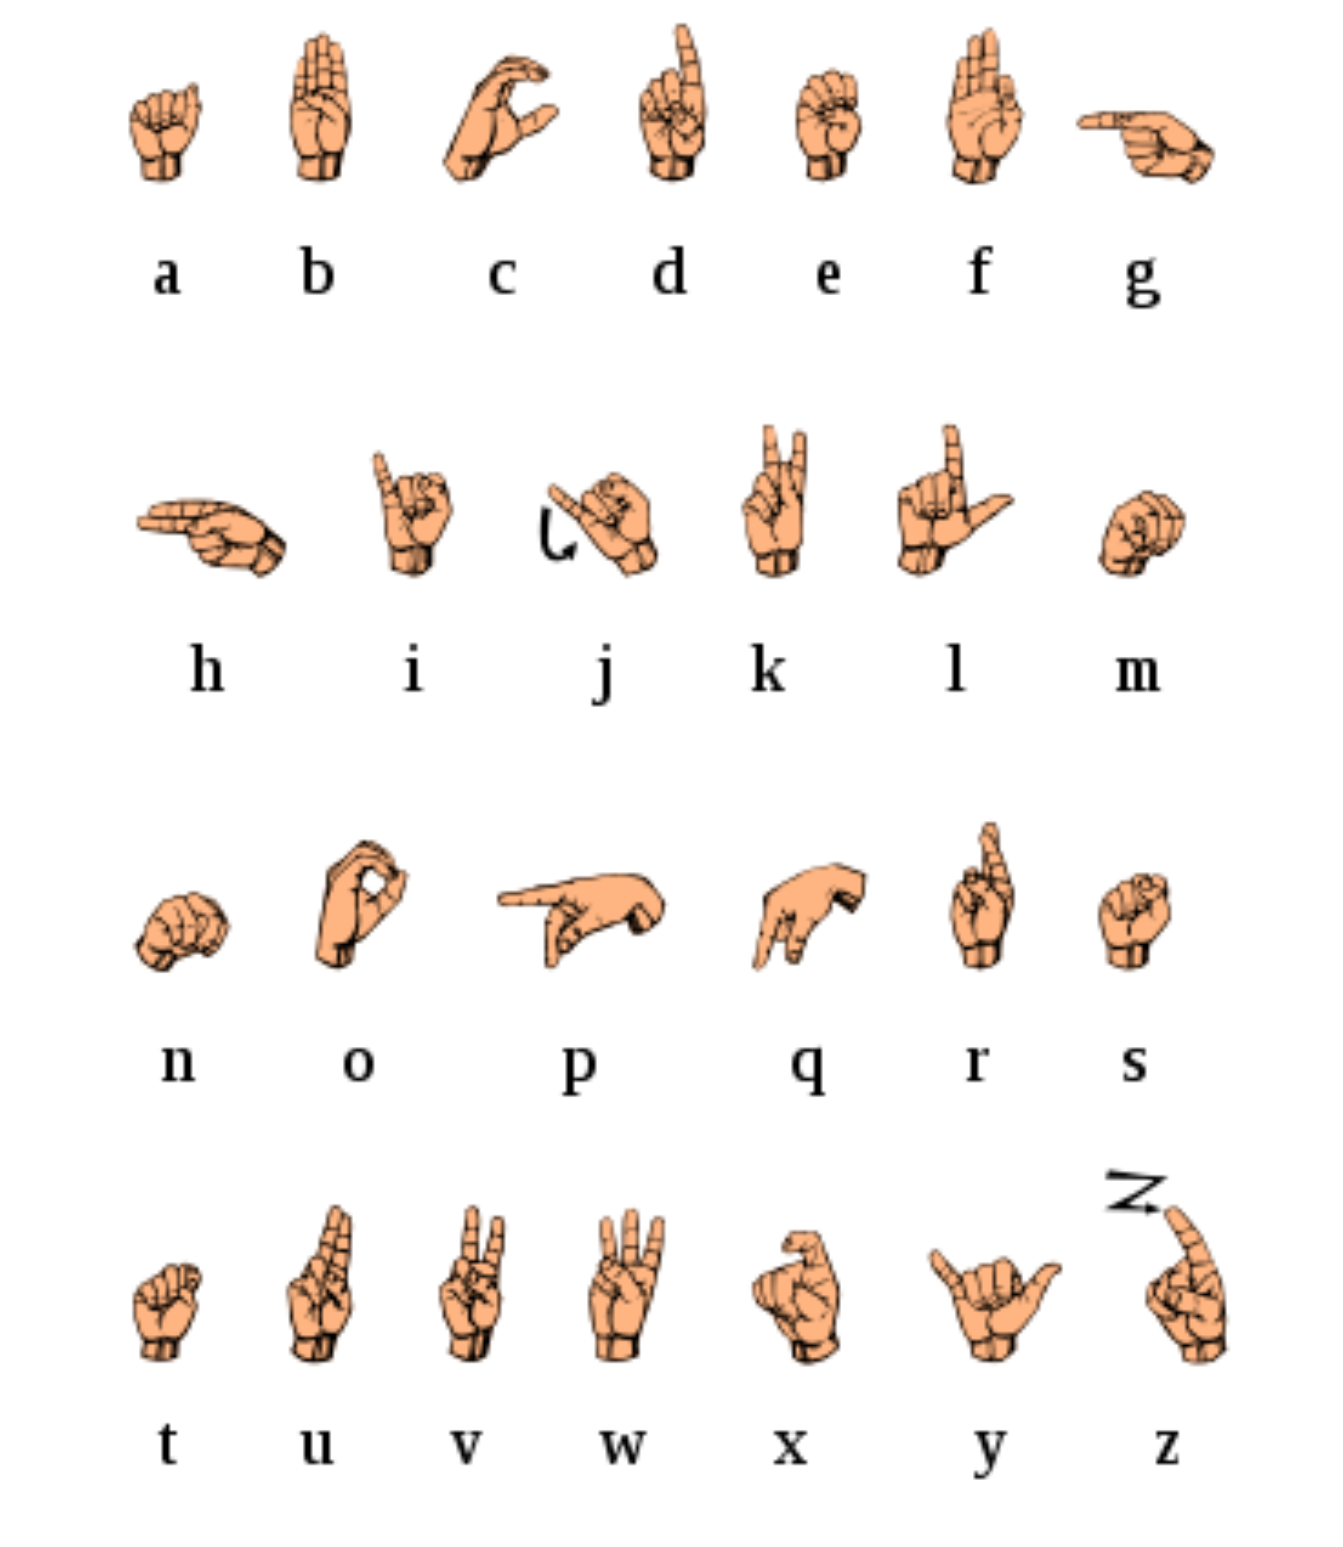
\includegraphics[width=1.0\textwidth]{fingeralphabet}
	\caption[Fingeralphabet]{Darstellung des Fingeralphabets \cite{FINGERALPHABET}.}
	\label{fig:fingeralphabet}
\end{figure}
\section{Eingrenzung}
Das Ergebnis dieses Projekts soll eine schriftliche Ausarbeitung und Quellcode für das Modell-Training sowie für ein Python Backend und Angular Frontend sein. Die Zeichenerkennung wurde auf das unter Abbildung \ref{fig:fingeralphabet} dargestellte amerikanische Fingeralphabet begrenzt. Umlaute oder Zahlen werden also nicht erkannt. Die Buchstaben J und Z sind zwar in einem der verwendeten Datensätze enthalten, erfordern aber eine gewisse Gestik, sodass die Erkennung in Standbildern erschwert ist. Da das hier vorgestellte Problem auf die Erkennung von Bildern zurückzuführen ist, wird in diesem Projekt auf Konvolutionelle Neuronale Netze gesetzt, welche im ImageNet Large Scale Visual Recognition Challenge (ILSVRC) die besten Ergebnisse erzielen. Vor Projektvergabe wurde auf einem kleinen Datensatz mit 28x28 Merkmalen eine Support Vektor Maschine mit RBF Kernel trainiert. Die erreichte Vorhersagegenauigkeit von ca. 79\% auf dem Testdatensatz wurde mit einem CNN aber schnell überboten. Zusätzlich wurde ein einfaches Neuronales Netz antrainiert, welches unter \ref{nntraining} beschrieben wird. Auch hier wurden Tests und Optimierungen aufgrund von ernüchternden Ergebnissen zügig abgebrochen und dienen in der Ausarbeitung nur als Vergleichswert. Im Rahmen der Vorlesung wurden unteranderem die Bibliotheken ScikitLearn, NumPy und Keras bearbeitet, sodass sich in der Projektarbeit größtenteils darauf beschränkt wird.  Die Nutzung der trainierten Modelle zielt darauf ab, Bilder einer Webcam in einem Intervall an ein Python Backend zu senden. Im Backend werden die bereits trainierten Modelle hinterlegt, welche dann eine Voraussage für das gesendete Bild treffen. Das Ergebnis entspricht einer Klassifikation, wobei jeder mögliche Buchstabe einer Klasse zugeordnet ist. Das Frontend soll als Antwort die jeweiligen Wahrscheinlichkeiten und den wahrscheinlichsten Buchstaben als separates Property bekommen welcher entsprechend im Frontend visualisiert wird. Das Python Backend gibt über einen Endpunkt die hinterlegten Modelle aus, sodass diese im Frontend jederzeit gewechselt werden können. Als Schnittstelle zwischen Frontend und Backend dienen einfache HTTP-Anfragen, sodass das Frontend ohne Probleme ausgetauscht oder durch ein weiteres ergänzt werden kann.
\section{Theoretische Grundlagen}
In diesem Abschnitt sollen theoretische Grundlagen des Maschinellen Lernens vorgestellt werden. Es wird zunächst auf allgemeine Grundlagen eingegangen, um im Folgenden Neuronale Netze und Konvolutionelle Neuronale Netze zu betrachten.
\subsection{Allgemeine Grundlagen des Maschinellen Lernens}
Maschinelles Lernen gibt einem Computer die Möglichkeit, Aufgaben zu erfüllen, ohne explizit von einem Entwickler für diese programmiert worden zu sein. Tom Mitchell beschreibt Maschinelles Lernen 1997 als ein Computerprogramm, das ohne Veränderungen des Programmcodes aus Erfahrungen E im Bezug auf eine Aufgabe T und ein Maß für die Leistung P lernt, indem seine Leistung P mit der Erfahrung E anwächst \cite[S. 4]{MACHINE_LEARNING}. Erfahrungen sammelt ein System, indem Daten mit speziellen Algorithmen betrachtet werden. Auf Basis dieser Daten erstellt der Algorithmus dann eine Strukturbeschreibung, die auch als Modell bezeichnet wird \cite[S. 2]{DEEP_LEARNING}.
\\\\
In diesem Projekt war die Aufgabe das Klassifizieren von Gebärdensprache. Die Leistung des Modells wird durch die korrekte Klassifizierung bestimmt, welche idealerweise während des Trainingsvorgangs beim Anlernen von Datensätzen zu Gebärdensprache ansteigen sollte.
\subsubsection{Arten von Verfahren des Maschinellen Lernens}
Verfahren des Maschinellen Lernens werden in der Literatur häufig mittels verschiedener Kategorien in unterschiedliche Arten aufgeteilt. Auch wenn viele Arten von Verfahren in dieser Arbeit nicht betrachtet werden, ist es wichtig, diese zu benennen, um ein passendes Verfahren auszuwählen. Es werden typischerweise drei Kategorien unterschieden, die Verfahren des Maschinellen Lernens einteilen \cite[S.8-14]{MACHINE_LEARNING}\cite[S.2]{BA}. 
\\\\
Zunächst wird ein Verfahren danach eingeteilt, welche Informationen zu den Trainingsdaten anhand von Labels nötig sind. Muss jeder Datenpunkt mit einem Label versehen sein, so handelt es sich um Überwachtes Lernen. Demgegenüber steht das Unüberwachte Lernen, bei dem ein Algorithmus versucht, Aussagen über mögliche Label anhand der Struktur der Daten zu treffen. Das Halbüberwachte Lernen kombiniert beide Eigenschaften und der Algorithmus versucht zunächst Label anzulernen, um im Folgenden autonom fortzufahren. Abschließend sei noch das Reinforcement Lernen zu nennen. Dieses bestraft und belohnt Aktionen auf eine vorher definierte Weise. Der Algorithmus versucht dann, möglichst viele Belohnungen in möglichst wenig Zeit zu erhalten und gleichzeitig Bestrafungen zu verhindern \cite[S.8-14]{MACHINE_LEARNING}\cite[S.2]{BA}.
\\\\
Eine weitere Kategorie ist die Art, wie ein Lernverfahren mit Daten versorgt werden muss. Beim Batch-Learning muss das Verfahren auf Basis eines kompletten Datensatzes trainiert und kann danach nicht mehr mit weiteren Daten verbessert werden. Es muss von Grund auf neu trainieren. Demgegenüber steht das Online-Learning, welches nach und nach trainiert wird, und noch eine spätere Verfeinerung ermöglicht \cite[S.14-17]{MACHINE_LEARNING}\cite[S.2]{BA}.
\\\\
Mit einer weiteren Kategorie wird festgelegt, wie ein Verfahren Daten verallgemeinert, um neue Aussagen treffen zu können. Beim Modellbasierten Lernen wird anhand der Daten ein mathematisches Modell erstellt, welches versucht, die Struktur der Daten korrekt zu beschreiben, um neue Vorhersagen treffen zu können. Instanzbasiertes Lernen vergleicht bei vorherzusagenden Daten die Merkmale mit bereits angelernten Datensätzen. Werden hier Ähnlichkeiten in den bereits erlernten Instanzen entdeckt, werden diese für eine neue Aussage genutzt \cite[S.14-17]{MACHINE_LEARNING}\cite[S.2]{BA}.
\\\\
Ebenfalls lassen sich Verfahren nach der Art des zu lösenden Problems einteilen. Bei der Klassifikation werden Daten anhand ihrer Labels einer gewissen Klasse zugeordnet. Das Ziel ist es nun, die Klasse von neuen Datensätzen korrekt vorherzusagen. Demgegenüber stehen Regressionsprobleme, bei denen ein Label einen konkreten Wert angibt, welcher bei einem neuen Datensatz vom Modell korrekt vorhergesagt werden muss \cite[S.8-9]{MACHINE_LEARNING}\cite[S.2]{BA}.
\\\\
Bei dem in dieser Arbeit zu lösenden Problem handelt es sich um ein typisches Klassifikationsproblem des Überwachten Lernens. Ein Modell wird auf Basis von vorklassifizierten Daten, also typischerweise Datensätze mit Bildern von Händen, die ein Zeichen in Gebärdensprache repräsentieren, angelernt. Dieses soll dann im Folgenden weitere Bilder einem Zeichen in Gebärdensprache korrekt zuweisen können. Instanzbasiertes Lernen könnte bei Bilddaten zu Problemen führen, da Bilder in der Regel relativ viele Daten beinhalten und dadurch zu sehr großen Modellen führen können \cite[S.18]{MACHINE_LEARNING}. Aus diesem Grund sollte Modellbasiertes Lernen vorgezogen werden. Es ist allerdings sowohl Batch-Learning, als auch Online-Learning denkbar.
\subsubsection{Typische Probleme beim Maschinellen Lernen}
Beim Maschinellen Lernen können viele Probleme auftreten, die den Lernerfolg eines Modells behindern können. Um diesen entgegenwirken zu können, sollten typische Probleme vor dem Entwickeln eines Modells betrachtet werden.
\\\\
Schon bei einfachen Problemen ist eine ausreichende Datenmengen nötig, um Modelle antrainieren zu können. Abhängig von der Komplexität eines Problems und des genutzten Algorithmus können Tausende bis Millionen von Datensätzen für einen Lernvorgang nötig sein \cite[S.23]{MACHINE_LEARNING}\cite[S.4]{BA}.
\\\\
Wurden Daten fehlerhaft gesammelt und repräsentieren nicht das Spektrum der möglichen Eingabe im Einsatz, so kann ein Modell keine korrekten Vorhersagen für den geplanten Einsatz treffen, da hier das Wertespektrum nicht das Gelernte repräsentiert. Auch eine ungünstige Verteilung von Klassen in den Daten kann zu Problemen führen; und zwar besonders dann, wenn dieser Fall mit unpassenden Qualitätsmaßen ausgewertet wird \cite[S.24-25]{MACHINE_LEARNING}\cite[S.4]{BA}.
\\\\
Minderwertige Daten erschweren ebenfalls den Lernvorgang. Dies kann sich durch verrauschte, fehlerhafte und fehlende Daten sowie Ausreißer äußern. Eine manuelle oder automatische Vorverarbeitung könnte dies verbessern. Sogar ein Auslassen bestimmter Merkmale kann sich als sinnvoll herausstellen. \cite[S.26]{MACHINE_LEARNING}\cite[S.3]{BA}. Hilft dies nicht, ist ein Sammeln von neuen Datensätzen sinnvoll.
\\\\
Irrelevante oder schlecht gewählte Merkmale für das Antrainieren eines Datensatzes führen ebenfalls zu einem schlechteren oder gar keinem Lernerfolg. Für das Vorhersagen von Gebärdensprache sollte zum Beispiel das Datum des vorherzusagenden Bildes keinen Einfluss haben. Wird diese Information im Trainingsvorgang trotzdem einbezogen, so ist mit einer schlechteren Performanz des Lernvorgangs zu rechnen \cite[S.26]{MACHINE_LEARNING}\cite[S.4]{BA}. 
\\\\
Overfitting tritt dann auf, wenn ein Modell für die Trainingsdaten zu komplex gewählt ist. Es führt dazu, dass ein Modell nicht korrekt verallgemeinert, sondern zufällige Variationen in den Trainingsdaten lernt. Es äußert sich in einer guten Performanz im Training, während diese in Tests nachlässt. Verhindern lässt sich dies im Modell durch eine Verringerung der Zahl der Parameter oder bestimmter Techniken, die dem Modell Restriktionen auflegen, der sogenannten Regularisierung. Außerdem lässt es sich durch Sammeln neuer Daten, sowie der Verringerung von Rauschen in bereits Vorhandenen reduzieren \cite[S.27]{MACHINE_LEARNING}\cite[S.13]{BA}.
\begin{figure}[H] 
	\centering
	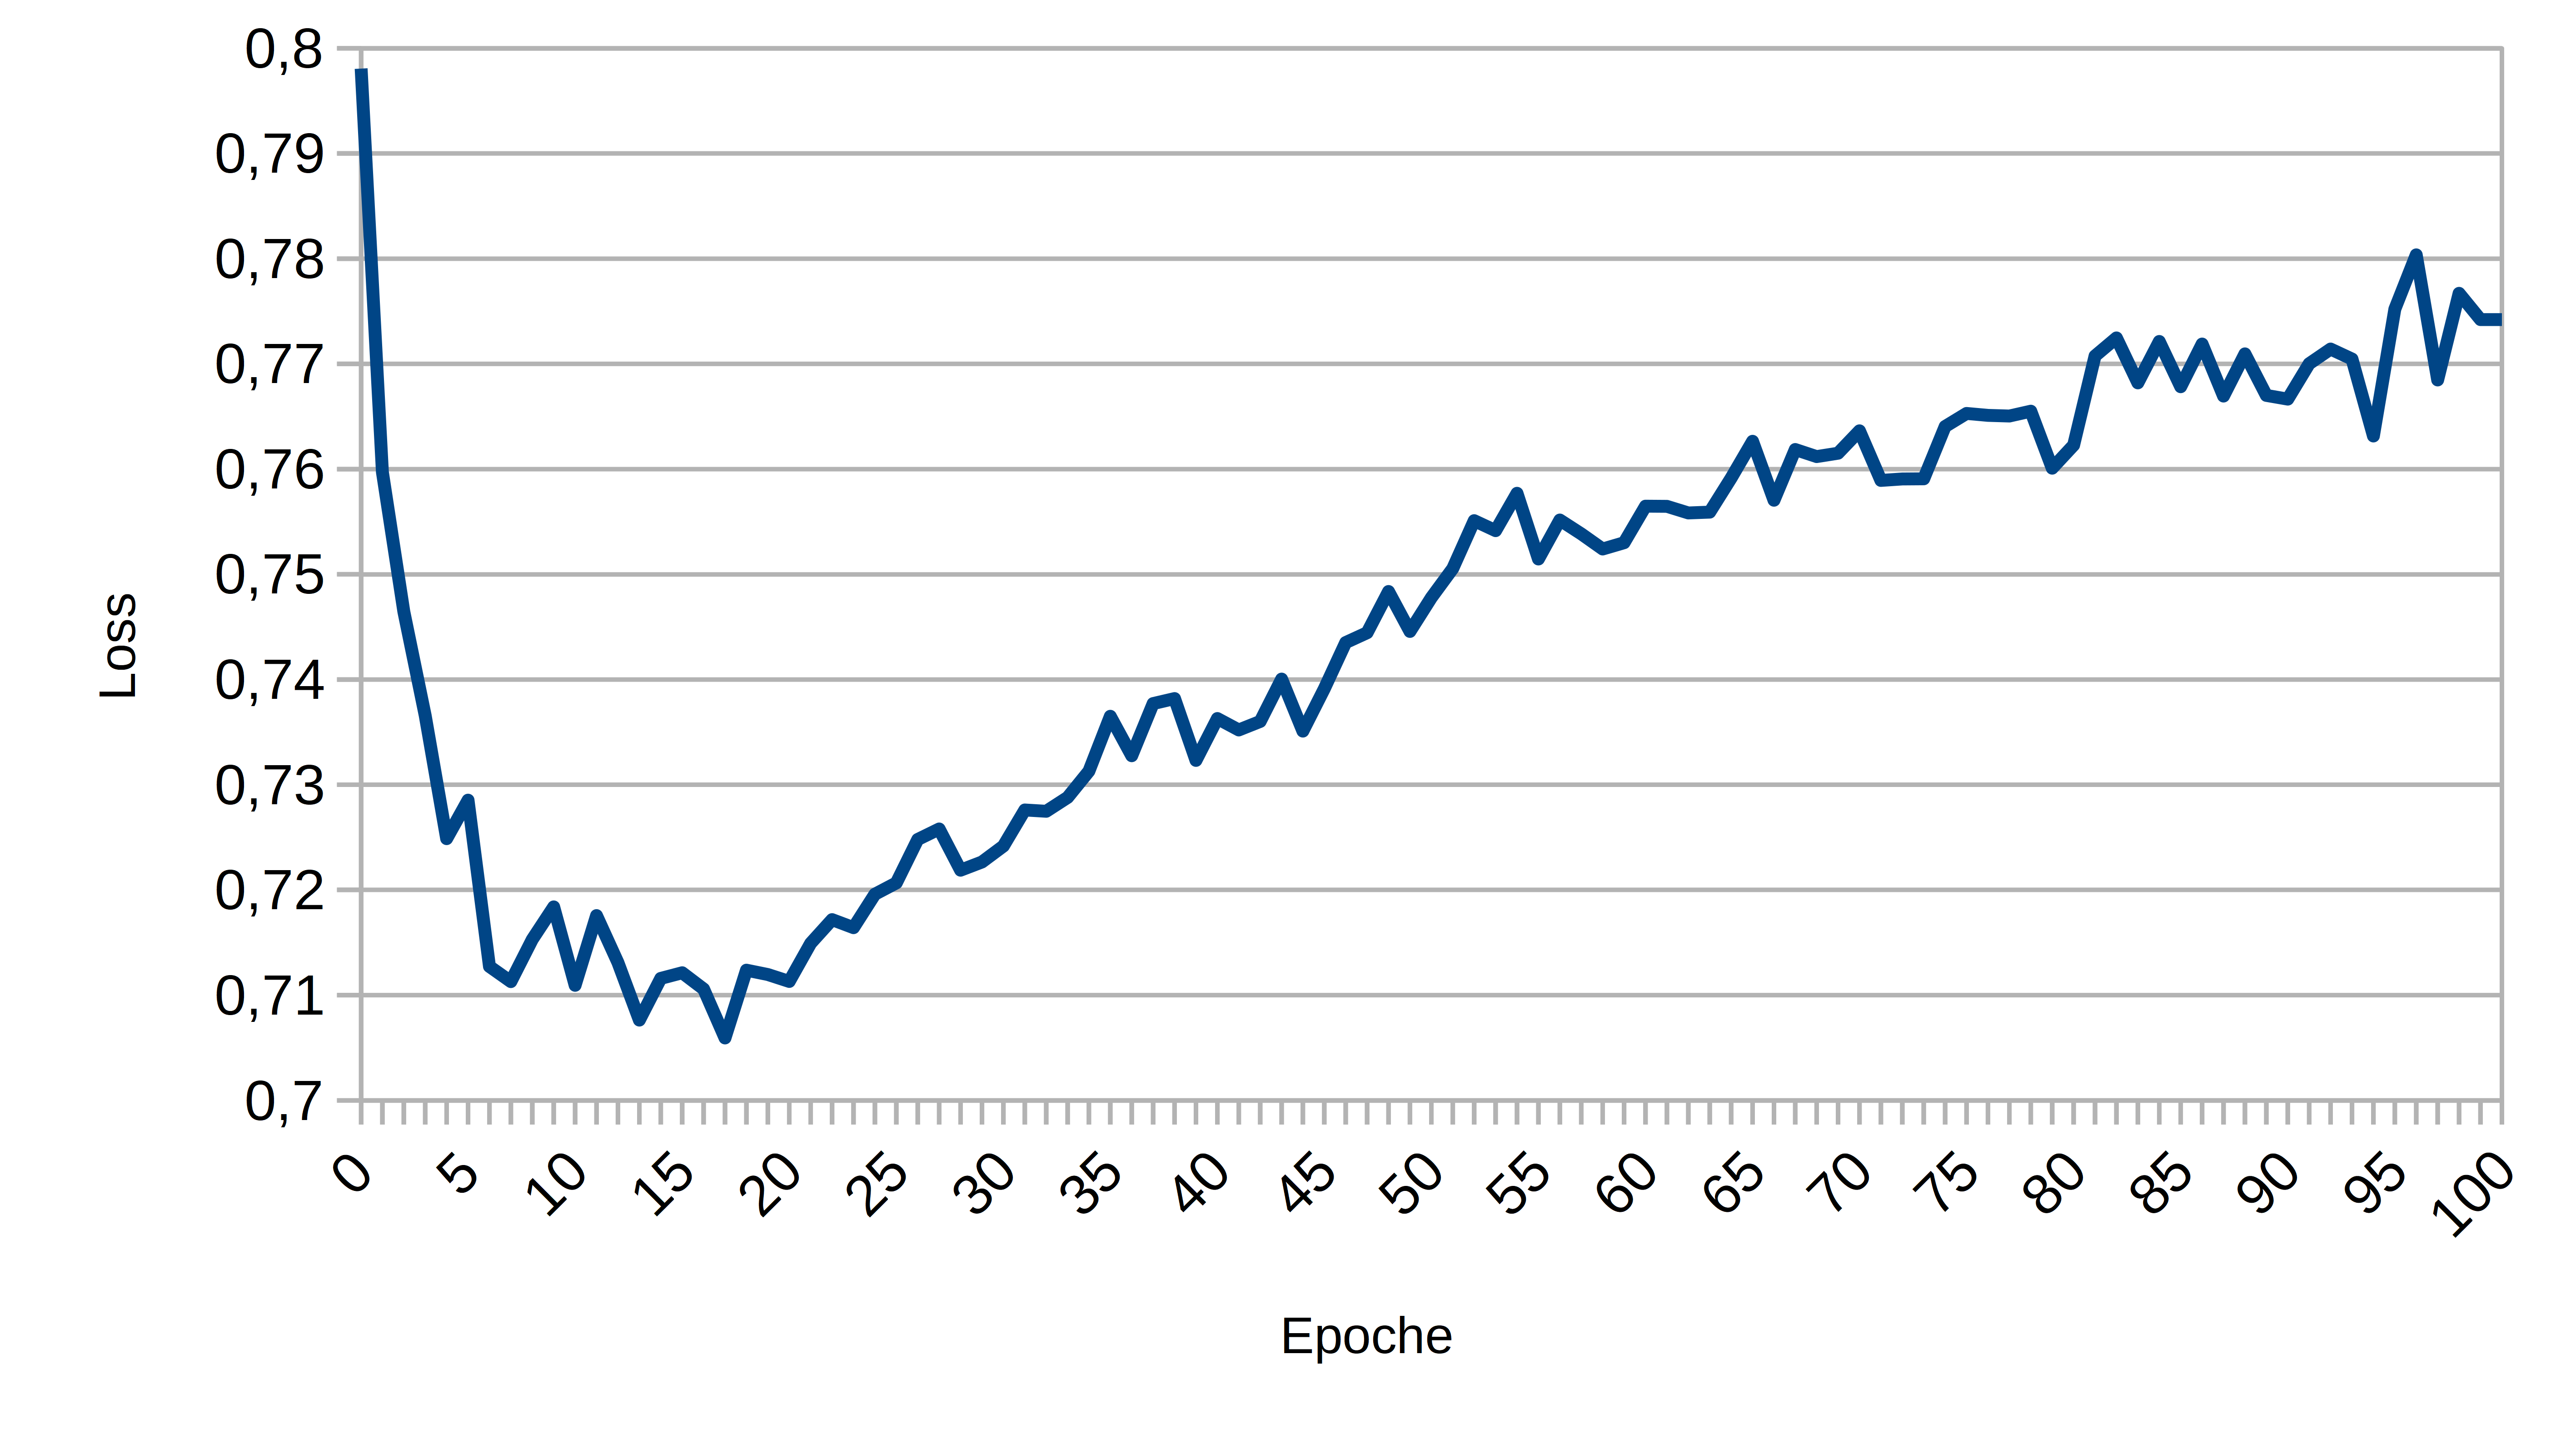
\includegraphics[width=1.0\textwidth]{mlp_5_loss}
	\caption[Overfitting in einem mehrschichtigen Neuronalen Netz]{Nach der 20. Epoche tritt in diesem mehrschichtigen Neuronalen Netz ein Overfitting auf \cite[S.14]{BA}.}
	\label{fig:mlp_overfitting}
\end{figure}
Zuletzt sei das Underfitting genannt, welches dem Overfitting gegenübersteht. Ein Modell ist dabei zu einfach, um die Strukturen in den Trainingsdaten anzulernen. Modelle mit mehr Parametern, bessere Merkmale oder eine Verringerung der Regularisierung reduzieren Underfitting in der Regel \cite[S.29]{MACHINE_LEARNING}\cite[S.14]{BA}.
\subsubsection{Datenvorverarbeitung für Bilddaten}
Wie im vorherigen Kapitel dargestellt, würden qualitativ unzureichende Daten zu einer schlechteren Performanz beim Anlernen eines Modells führen. Dies kann auch bei Bilddaten der Fall sein und sollte durch Vorverarbeitungsschritte verhindert werden. In dieser Sektion sollen einige typische Schritte der Bildvorverarbeitung dargestellt werden.
\\\\
Verrauschte Bilder können bei der Bilderkennung große Probleme darstellen. Ist ein Bild nicht rauschfrei, wurde gezeigt, dass Verfahren zum Entfernen von Rauschen eine positiven Effekt haben können \cite{RAUSCH}. Dieses Verfahren wurde im Praxisteil zwar aufgrund des qualitativ hochwertigen Datensatzes nicht genutzt, stellt aber für die Zukunft, besonders im Einsatz, wo die Qualität der Bilddaten nicht immer gewährleistet ist, eine gute Methode für eine möglichen Verbesserung dar.
\\\\
Ein weiterer Datenvorverarbeitungsschritt ist das Extrahieren von relevanten Bildausschnitten. Die meisten Datensätze für die Erkennung von Gebärdensprache haben hier bereits die relevanten Ausschnitte vorverarbeitet, sodass nur noch die Hände zu sehen sind. Dies ist jedoch ein Problem für die Praxis, da ein Bild einer Webcam in der Regel mehr als nur die Hand beinhaltet. Es würde hier das Problem entstehen, dass die Daten in der Praxis nur wenig mit dem Angelernten übereinstimmen. Hier ist es also sinnvoll, den relevanten Teil eines Bildes zu extrahieren. Dazu wurde im Praxisteil ein Machine-Learning Framework namens MediaPipe genutzt \cite{MEDIAPIPE}.
\\\\
Zuletzt müssen Bilder in der Regel vor der Nutzung skaliert werden. Modelle des Maschinellen Lernens erwarten in der Regel eine feste Eingabegröße. Dies gilt auch für Bilder, sodass beispielsweise das VGG19 Konvolutionelle Neuronale Netzwerk für Objekterkennung eine Eingabegröße von 224 x 224 Pixeln erwartet \cite[S.2]{SCALE}. Auch mit Blick auf die Laufzeit ergibt eine Skalierung von Bildern Sinn. Moderne Webcams erreichen häufig schon eine Auflösung von 1920 x 1080 Pixeln. Dies würde bei unskalierten und nicht extrahierten Bildinformationen zu einer Eingabegröße von 2. Millionen Parametern führen, was abhängig vom Modell zu sehr hohen Laufzeiten führen kann. Typische Algorithmen zum Herunterskalieren von Bildern sind die Nächste-Nachbarn, Bilineare und Bikubische Interpolation \cite[S.2]{SCALE}.
\subsubsection{Qualitätsmaße}
Um die Leistung eines Modells korrekt bewerten zu können, müssen abhängig vom Ziel Qualitätsmaße eingeführt werden, die es möglich machen, Modelle untereinander zu vergleichen. Dazu wird mit der Kreuzentropie ein typisches Qualitätsmaß für Klassifikationsprobleme eingeführt. Außerdem werden die Begriffe Konfusionsmatrix, Accuracy, Precision, Recall und F1-Score diskutiert.
\\\\
In praktisch allen Fällen können Algorithmen des Maschinellen Lernens nicht mit Klassenbezeichnungen in Form von Zeichenketten umgehen. Eine Menge von Klassenbezeichnungen wie \ensuremath{\{a, b, c \}} könnte nur schwierig direkt von Algorithmen als Label genutzt werden. Hier werden in der Regel zwei Möglichkeiten genutzt, um Bezeichnungen in nützlichere Label umzuwandeln. Diese wären:
\begin{itemize}
	\item Klassen-IDs: Die vorher angegebene Menge von Klassenbezeichnungen könnte in eine Menge von repräsentierenden IDs transformiert werden. So wird die Menge \ensuremath{\{a, b, c \}} in die IDs \ensuremath{\{0, 1, 2 \}} umgewandelt. Der Algorithmus muss bei der Klassifikation nun eine korrekte IDs vorhersagen, welche eine Klasse repräsentiert. Aufgrund der Arbeitsweise vieler Algorithmen nehmen diese allerdings an, dass IDs, die näher beieinander liegen, zueinander ähnlicher sind. Dies ist nicht für alle Problemstellungen ideal \cite[S.12]{BA}\cite[S.63]{MACHINE_LEARNING}.
	\item One-Hot-Kodierung: Bei diesem Verfahren wird für jede Klasse eine Zahl in einem Vektor reserviert. Eine vorliegende Klasse wird dann in der Regel mit einer 1 und der Rest der Elemente mit einer 0 markiert. Für die Beispielmenge \ensuremath{\{a, b, c \}} ergäbe sich daher die Menge von Vektoren \ensuremath{\{\left(\begin{smallmatrix}1 & 0 & 0\end{smallmatrix}\right), \left(\begin{smallmatrix}0 & 1 & 0\end{smallmatrix}\right), \left(\begin{smallmatrix}0 & 0 & 1\end{smallmatrix}\right)\}}. Korrekt klassifiziert wurde nun, wenn die vorliegenden Klassen mit den höchsten Vorhersagen markiert werden. Da in diesem Fall keine Beziehung zwischen den Klassen erkannt wird, ist diese Darstellung auch ideal für die betrachtete Problemstellung \cite[S.12]{BA}\cite[S.63]{MACHINE_LEARNING}.
\end{itemize}
Die bereits vorher erwähnte Kreuzentropie ist ein ideales Qualitätsmaß für Klassifikationsprobleme in der One-Hot-Kodierung. Niedrige Vorhersagen bei den vorliegenden Klassen werden dabei abgestraft, während andere Vorhersagen ignoriert werden. Für einen Datensatz mit \ensuremath{m} Tupeln, seinen One-Hot-kodierten Labels \ensuremath{\textbf{y}} mit \ensuremath{K}-Klassen und den One-Hot-kodierten Vorhersagen \ensuremath{\textbf{y'}} mit \ensuremath{K}-Klassen gilt \cite[S.13]{BA}\cite[S.63]{MACHINE_LEARNING}:
\begin{equation}
\label{eq:crossentropy}
J = -\frac{1}{m}\sum_{i=1}^{m}\sum_{k=1}^{K}\textbf{y}_{ik} \cdot \log({\textbf{y}'_{ik}})
\end{equation}\myequations{Kreuzentropie}
\\
Nun wurde ein Qualitätsmaß eingeführt, mit dem die Korrektheit einer Vorhersage bestimmt werden kann. Im Folgenden werden nun Wege beschrieben, wie sich die Performanz eines Modells auf einem gesamten Datensatz auswerten lässt. Eine typische und ausführliche Auswertungsmöglichkeit bei Klassifikationsproblemen ist eine Konfusionsmatrize, für die ein Beispiel in Abbildung \ref{fig:konfusion} zu sehen ist. Jede Zeile in einer Konfusionsmatrize steht für eine tatsächliche Klasse, während eine Spalte eine vorhergesagte Kategorie repräsentiert (dies ist definitionsabhängig und kann auch getauscht werden). Die Wertepunkte in der Matrize beschreiben damit, als welche Klasse ein Datenpunkt einer tatsächlichen Klasse vorhergesagt wird. Sie werden meistens als feste Anzahl oder Anteile in Prozent aller Vorhersagen zu dieser Klasse angegeben. Die Hauptdiagonale der Matrize beschreibt alle korrekt klassifizierten Vorhersagen \cite[S.86-87]{MACHINE_LEARNING}.
\begin{figure}[H]
	\begin{center}
		\begin{tabular}{|c||c|c|c|}
			\hline
			 & A & B & C\\
			\hhline{|=||=|=|=|}
			A & 90 & 4 & 6\\
			\hline
			B & 12 & 85 & 2\\
			\hline	
			C & 4 & 19 & 80\\
			\hline
		\end{tabular}
	\end{center}
	\caption[Beispiel einer Konfusionsmatrize]{Beispiel einer Konfusionsmatrize für die Klassen A, B, C.}
	\label{fig:konfusion}
\end{figure}
Eine Konfusionsmatrize ist sehr ausführlich und beinhaltet besonders bei vielen Klassen viele Informationen, die nicht unbedingt für die Lösung des betrachteten Problems relevant sind. In diesem Fall können andere Qualitätsmaße sinnvoll sein. Um diese zu errechnen, ist ein Verständnis über die Begriffe True Positive (TP), True Negative (TN), False Positive (FP) und False Negative (FN) nötig \cite[S.87]{MACHINE_LEARNING}. Diese sind beispielsweise, abhängig von Klasse A, in der Abbildung \ref{fig:konfusion_tp} zu erkennen. Es gilt:
\begin{itemize}
	\item True Positive (grün): Beschreibt den korrekt klassifizierten Anteil der betrachteten Klasse.
	\item True Negative (hellgrün): Beschreibt den korrekt klassifizierten Anteil der nicht betrachteten Klassen. 
	\item False Positive (rot): Beschreibt den Anteil, mit dem die nicht betrachteten Klassen fälschlicherweise als die Betrachtete eingeordnet werden.
	\item False Negative (orange): Beschreibt den Anteil, mit dem eine betrachtete Klasse fälschlicherweise als die nicht betrachteten Klassen eingeordnet wird.
\end{itemize}
\begin{figure}[H]
	\begin{center}
		\begin{tabular}{|c||c|c|c|}
			\hline
			& A & B & C\\
			\hhline{|=||=|=|=|}
			A & {\cellcolor{green_tp}} 90 & {\cellcolor{red_fn}} 4 & {\cellcolor{red_fn}} 6\\
			\hline
			B & {\cellcolor{red_fp}} 12 & {\cellcolor{green_tn}} 85 & 2\\
			\hline	
			C & {\cellcolor{red_fp}} 4 & 19 & {\cellcolor{green_tn}} 80\\
			\hline
		\end{tabular}
	\end{center}
	\caption[Klassenweises Beispiel für TP, TN, FN, FP in einer Konfusionsmatrize]{Beispiel für TP, TN, FN, FP der Klasse A in einer Konfusionsmatrize.}
	\label{fig:konfusion_tp}
\end{figure}
Nun können auf Basis der eingeführten Begriffe einige Qualitätsmaße eingeführt und ihr Einsatz abhängig vom Datensatz diskutiert werden. Die Vorhersagegenauigkeit A stellt alle korrekt klassifizierten Datenpunkte (TP, TN), der Menge aller klassifizierten Datenpunkte (M) gegenüber \eqref{eq:vorhersageg}. Die Vorhersagegenauigkeit ist ein beliebtes Qualitätsmaß, welches jedoch einige Probleme aufweist. Ist ein Datensatz unbalanciert, ist eine Klasse also deutlich mehr vertreten als eine andere, so wird diese Klasse die Vorhersagegenauigkeit stärker beeinflussen als andere. Dies kann zu einem Klassifikator führen, der lediglich die am stärksten vertretene Klasse antizipiert \cite[S.85-86]{MACHINE_LEARNING}.
\begin{equation}
\label{eq:vorhersageg}
\begin{aligned}
&A = \frac{TP + TN}{M}
\end{aligned}
\end{equation}\myequations{Vorhersagegenauigkeit} \\
Der Recall \eqref{eq:recall} ist ein Maß, welches die korrekt klassifizierten Datenpunkte allen Datenpunkten mit dieser Klasse gegenüberstellt. Er ist damit sehr gut für unterrepräsentierte Klassen geeignet, da ein Fokus auf die korrekte Klassifikation gesetzt wird \cite[S.87]{MACHINE_LEARNING}. Ein möglicher Anwendungsfall wäre damit die korrekte Klassifikation von Krankheitsfällen, da diese in der Regel unterrepräsentiert sind.
\begin{equation}
\label{eq:recall}
\begin{aligned}
&R = \frac{TP}{TP + FN}
\end{aligned}
\end{equation}\myequations{Recall} \\
Weiterhin gibt es mit der Precision \eqref{eq:precision} ein Qualitätsmaß, welches dem Recall mit einer Wechselbeziehung gegenübersteht. Statt die False Negatives zu betrachten, betrachtet es mit den False Positives die Datenpunkte, die fälschlicherweise als die betrachtete Klasse klassifiziert wurden. Die Precision steigt also, wenn weniger Datenpunkte falsch als die betrachtete Klasse dargestellt werden \cite[S.87]{MACHINE_LEARNING}. Ein typischer Anwendungsfall hierfür ist ein Spamfilter, da möglichst wenig Nachrichten fälschlicherweise als Spam markiert werden sollten.
\begin{equation}
\label{eq:precision}
\begin{aligned}
&P = \frac{TP}{TP + FP}
\end{aligned}
\end{equation}\myequations{Precision} \\
Zuletzt sei mit dem F1-Score \eqref{eq:fone} ein beliebtes Qualitätsmaß genannt, welches Recall und Precision in ihrem harmonischen Mittelwert vereint. Es wird genutzt, wenn sowohl Recall als auch Precision relevante Tatsachen darstellen.
\begin{equation}
\label{eq:fone}
\begin{aligned}
&F1 = 2\cdot \frac{P \cdot R}{P + R}
\end{aligned}
\end{equation}\myequations{F1-Score} \\ 
Da nun alle typischen Qualitätsmaße eingeführt wurden, können im nächsten Kapitel typische Richtlinien zum Vergleichen der Performanz von Modellen beschrieben werden.
\subsubsection{Testen und Validieren}
\label{validation}
Eine gute Performanz während des Trainings eines Modells bedeutet noch keine gute tatsächliche Leistung. Overfitting oder andere Effekte können eine Qualität vortäuschen, welche im echten Einsatz aufgrund einer Spezialisierung des Modells auf die Trainingsdaten nicht erreicht wird. Es haben sich hier zwei typische Verfahren etabliert, um damit umzugehen:
\\\\
Zum einen kann ein Trainingsdatensatz in drei Teile, einen tatsächlichen Trainingsdatensatz, einen Validierungsdatensatz und einen Testdatensatz unterteilt werden. Eine typische Unterteilung hierfür ist, 80\% für das Training und jeweils 10\% für Validierung und Test zu reservieren. Das Modell wird dann wie bisher mit dem Trainingsdatensatz angelernt und im Folgenden mit dem Valdierungsdatensatz geprüft. Dann wird das Modell optimiert und der Vorgang wiederholt, bis die gewünschte Qualität erreicht wurde. Ist dies  abgeschlossen, ist eine letzte Überprüfung nötig. Da während des Optimierungsvorgangs eine Spezialisierung auf Trainings- und Validierungsdaten stattgefunden haben könnte, muss mit dem bisher unbekannten Testdatensatz eine erreichte Verallgemeinerung des Wissens im Modell überprüft werden. Wurde keine ausreichende Performanz festgestellt, muss der gesamte Trainingsvorgang wiederholt werden, bis ein Modell die gewünschte Qualität erreicht hat \cite[S.30-31]{MACHINE_LEARNING}\cite[S.43-44]{BA}.
\\\\
Eine weitere beliebte Möglichkeit zur Validierung von Modellen ist die Kreuzvalidierung. Ein Datensatz wird dabei in k-Teile (beispielsweise k = 10) unterteilt. Einer dieser Teile wird als Testdatensatz ausgewählt, während alle anderen Teile zum Training kombiniert werden. Dann wird das Training ausgeführt und die Leistung des Modells vermerkt. Nun wird dies für einen anderen der k-Teile als Testdatensatz und dem nicht trainierten Modell wiederholt, bis jeder Teil einmal getestet wurde. Aus den k-Leistungsdaten wird dann eine Gesamtleistung errechnet, welche eine gute Repräsentation für die Leistung des Modells ist. Zum genaueren Testen nach der Kreuzvalidierung ist auch eine vorherige Abspaltung weiterer Testdaten denkbar \cite[S.22]{DEEP_LEARNING}\cite[S.44]{BA}.
\begin{figure}[H]
	\centering
	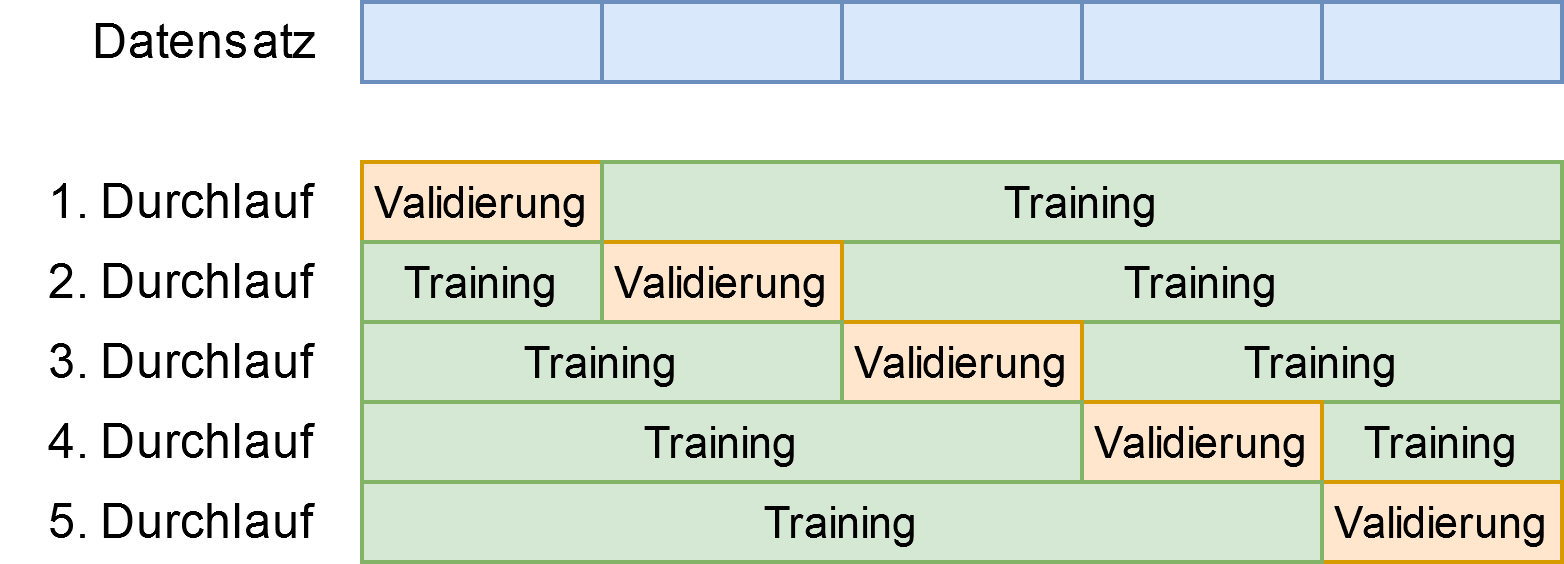
\includegraphics[width=0.90\textwidth]{kreuzvalidierung}
	\vspace*{-3mm}
	\caption[Beispiel für Kreuzvalidierung]{Beispiel für eine 5-fache Kreuzvalidierung \cite[S.44]{BA}.}
	\label{fig:crossvalidation}
\end{figure}
\vspace*{-5mm}
\subsection{Neuronale Netze}
In dieser Arbeit wurde sich, wie heutzutage üblich, bei der Bilderkennung auf Neuronale Netze und besonders die Konvolutionellen Neuronalen Netze fokussiert. Diese sind bei der Bilderkennung in vielen Bereichen State of the Art und werden von vielen bekannten vortrainierten Modellen wie dem VGG19 genutzt. Um diese zu verstehen, sollen allerdings erst die Grundlagen der Neuronalen Netze betrachtet werden.
\subsubsection{Biologische Grundlagen}
Neuronen sind für viele Menschen vor allem aus ihren eigenen Gehirn bekannt. In diesem arbeiten viele der kleinen Nervenzellen zusammen, um Informationen zu verarbeiten. Jedes Neuron nimmt elektrische Signale über seine stark verzweigten Dendriten auf und sammelt sie in seinem Zellkörper, dem Soma, an. Ist eine gewissen Stärke des elektrischen Signals vorhanden, so gibt ein Neuron dieses über sein Axon weiter. Axone sind lange, verzweigte Fäden, die mittels Synapsen mit den Dendriten anderer Neuronen verbunden sind. Synapsen arbeiten mit chemischen Transmittern und können eine erregende oder hemmende Wirkung auf das zu übertragene Signal haben. Biologische Neuronale Netze lernen nun, indem die Stärke der Verbindung über die Synapsen gesteuert wird. Außerdem können Verbindungen getrennt und neu eingegangen werden, was ebenfalls einen Lerneffekt erzeugt \cite[S.24]{BA}\cite[S.43-45]{DEEP_LEARNING}\cite[S.29-30]{NNP}.
\begin{figure}[H]
	\centering
	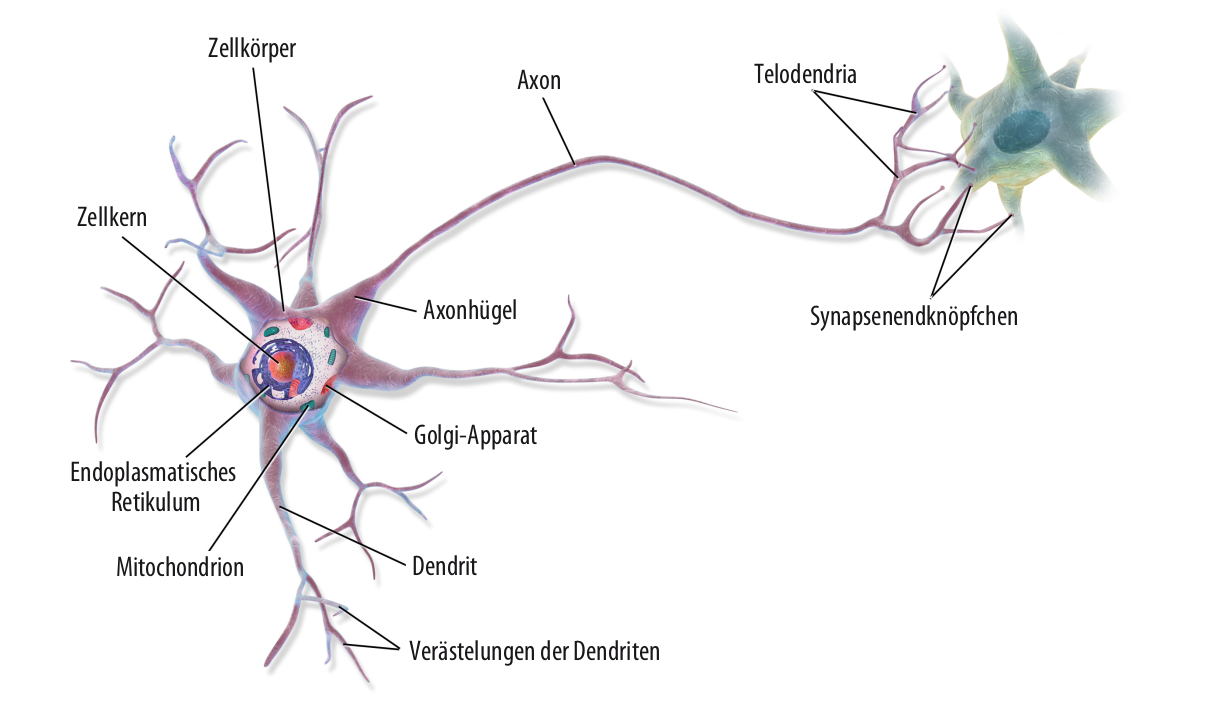
\includegraphics[width=1\textwidth]{neuron_biologisch}
	\vspace*{-5mm}
	\caption[Aufbau eines biologischen Neurons]{Aufbau eines biologischen Neurons \cite[S.255]{MACHINE_LEARNING}.}
	\label{fig:aufbau_bio_neuron}
\end{figure}
\vspace*{-5mm}
\subsubsection{Künstliche Neuronen}
In künstlichen Neuronalen Netzen wird nun eine auf den biologischen Grundlagen basierende künstliche Variante von Neuronen genutzt. Diese nehmen über ihre Eingänge, ähnlich zu den verbundenen Axonen, Signale auf, welche als ein Vektor \textbf{x} mit n-Elementen dargestellt werden. Jedes dieser Eingangssignale wird nun über einen eigenen Wert in einem Gewichtungsvektor \textbf{w} gehemmt oder verstärkt, was ähnlich zu der Arbeitsweise von Synapsen ist. Nun werden ebenfalls, ähnlich zum biologischen Vorbild, alle eingegangenen Signale aufaddiert, jedoch an eine Aktivierungsfunktion \ensuremath{f_{akt}} weitergegeben, welche ein Signal nochmal auf eine bestimmte Weise verarbeitet und sich komplett anders zum biologischen Vorbild verhalten kann. Zum Schluss kann das errechnete Signal des Künstlichen Neurons an weitere Neuronen, ähnlich zum ausgehenden Axon der biologischen Variante, weitergeleitet werden \cite[S.25]{BA}\cite[S.30-31]{NNP}.
\begin{figure}[H]
	\centering
	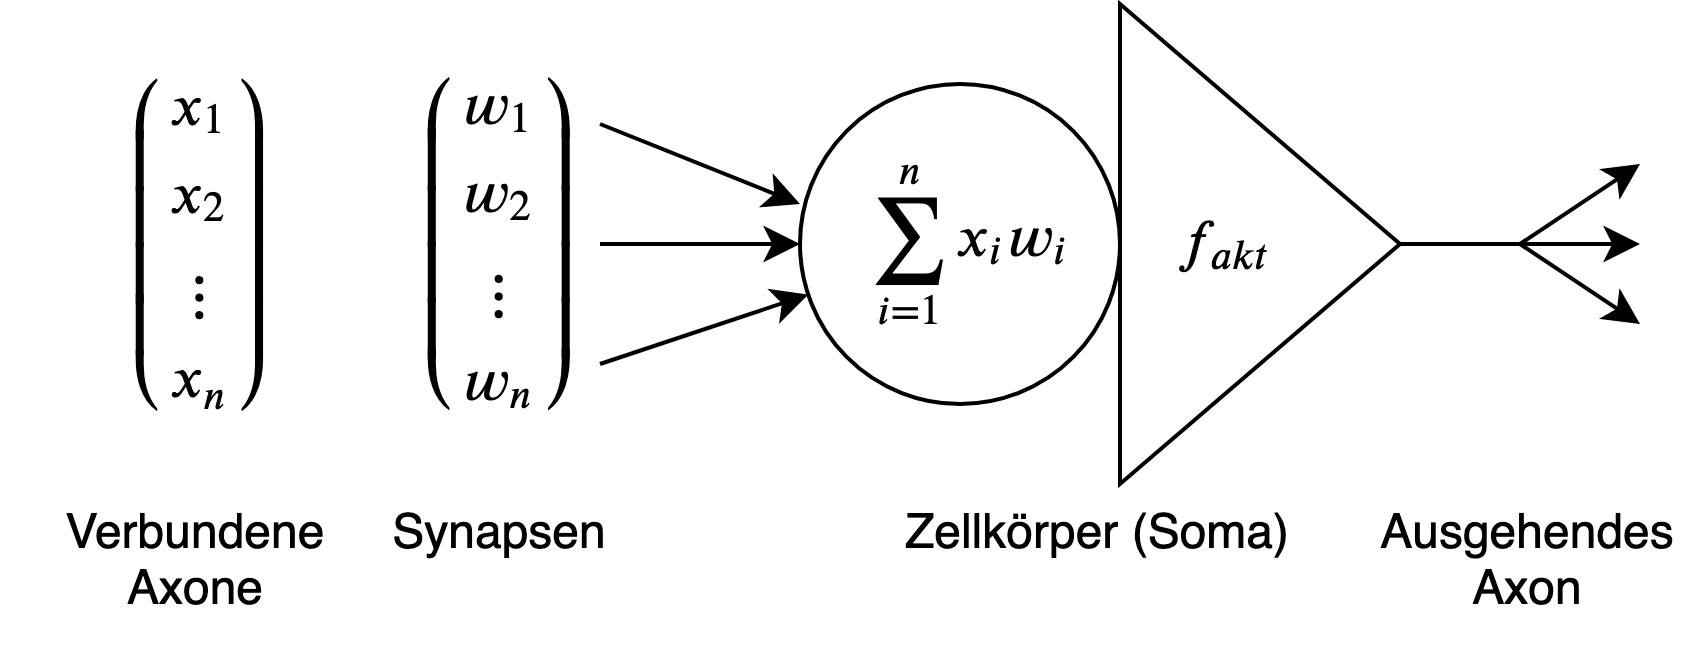
\includegraphics[width=1\textwidth]{neuron_adv}
	\vspace*{-5mm}
	\caption[Aufbau eines künstlichen Neurons]{Aufbau eines künstlichen Neurons, angelehnt an das biologische Vorbild \cite[S.25]{BA}.}
	\label{fig:aufbau_kuenstliches_neuron}
\end{figure}
\vspace*{-5mm}
Für n Eingänge lässt sich ein Künstliches Neuron nun folgendermaßen definieren \cite[S.25]{BA}\cite[S.30]{NNP}:
\begin{equation}
\label{eq:perceptron_def}
\begin{aligned}
y = f_{akt}\left(\sum_{i=1}^{n}x_iw_i\right) = f_{akt}(\textbf{x}^T \cdot \textbf{w})
\end{aligned}
\end{equation}\myequations{Mathematische Definition eines Künstlichen Neurons}\\
Wird eine Schwellenwertfunktion \eqref{eq:heavyside} als Aktivierungsfunktion genutzt, so wird ein Künstliches Neuron in der Regel als Perzeptron bezeichnet \cite[S.26]{BA}\cite[S.49]{DEEP_LEARNING}. 
\begin{equation}
\label{eq:heavyside}
\begin{aligned}
f_{akt} =
\begin{cases}
0 & x < 0\\
1 & x \geq 0
\end{cases}
\end{aligned}
\end{equation}\myequations{Schwellenwertfunktion eines Perzeptrons}
\subsubsection{Einschichtige Neuronale Netze}
Liegen mehrere Künstliche Neuronen oder Perzeptrons in einer einzigen Schicht vor, entsteht ein einschichtiges Neuronales Netz. Dabei wird jeder Eingang in das Neuronale Netz mit jedem Neuron in der Schicht des Netzes verbunden und über Gewichtungen verändert. Die Eingänge werden dabei häufig in der Notation als Schicht von Eingabeneuronen dargestellt, welche lediglich die Eingabewerte an die Künstlichen Neuronen weitertragen. Weiterhin wird in die Eingabeschicht dieser Netze häufig ein spezielles Neuron eingeführt, welches lediglich eine Eins als Ausgabe liefert und über Gewichtungen verändert werden kann. Dies wird als Bias-Neuron bezeichnet. Die Ausgänge der Künstlichen Neuronen des Netzes können nun als Ausgabevektor \textbf{y} ausgelesen werden \cite[S.26]{BA}\cite[S.258]{MACHINE_LEARNING}. Ein einschichtiges Neuronales Netz mit einer vereinfachten Darstellung der Neuronen ist in der Abbildung \ref{fig:multi_neuron_perceptron} dargestellt.
\begin{figure}[H]
	\centering
	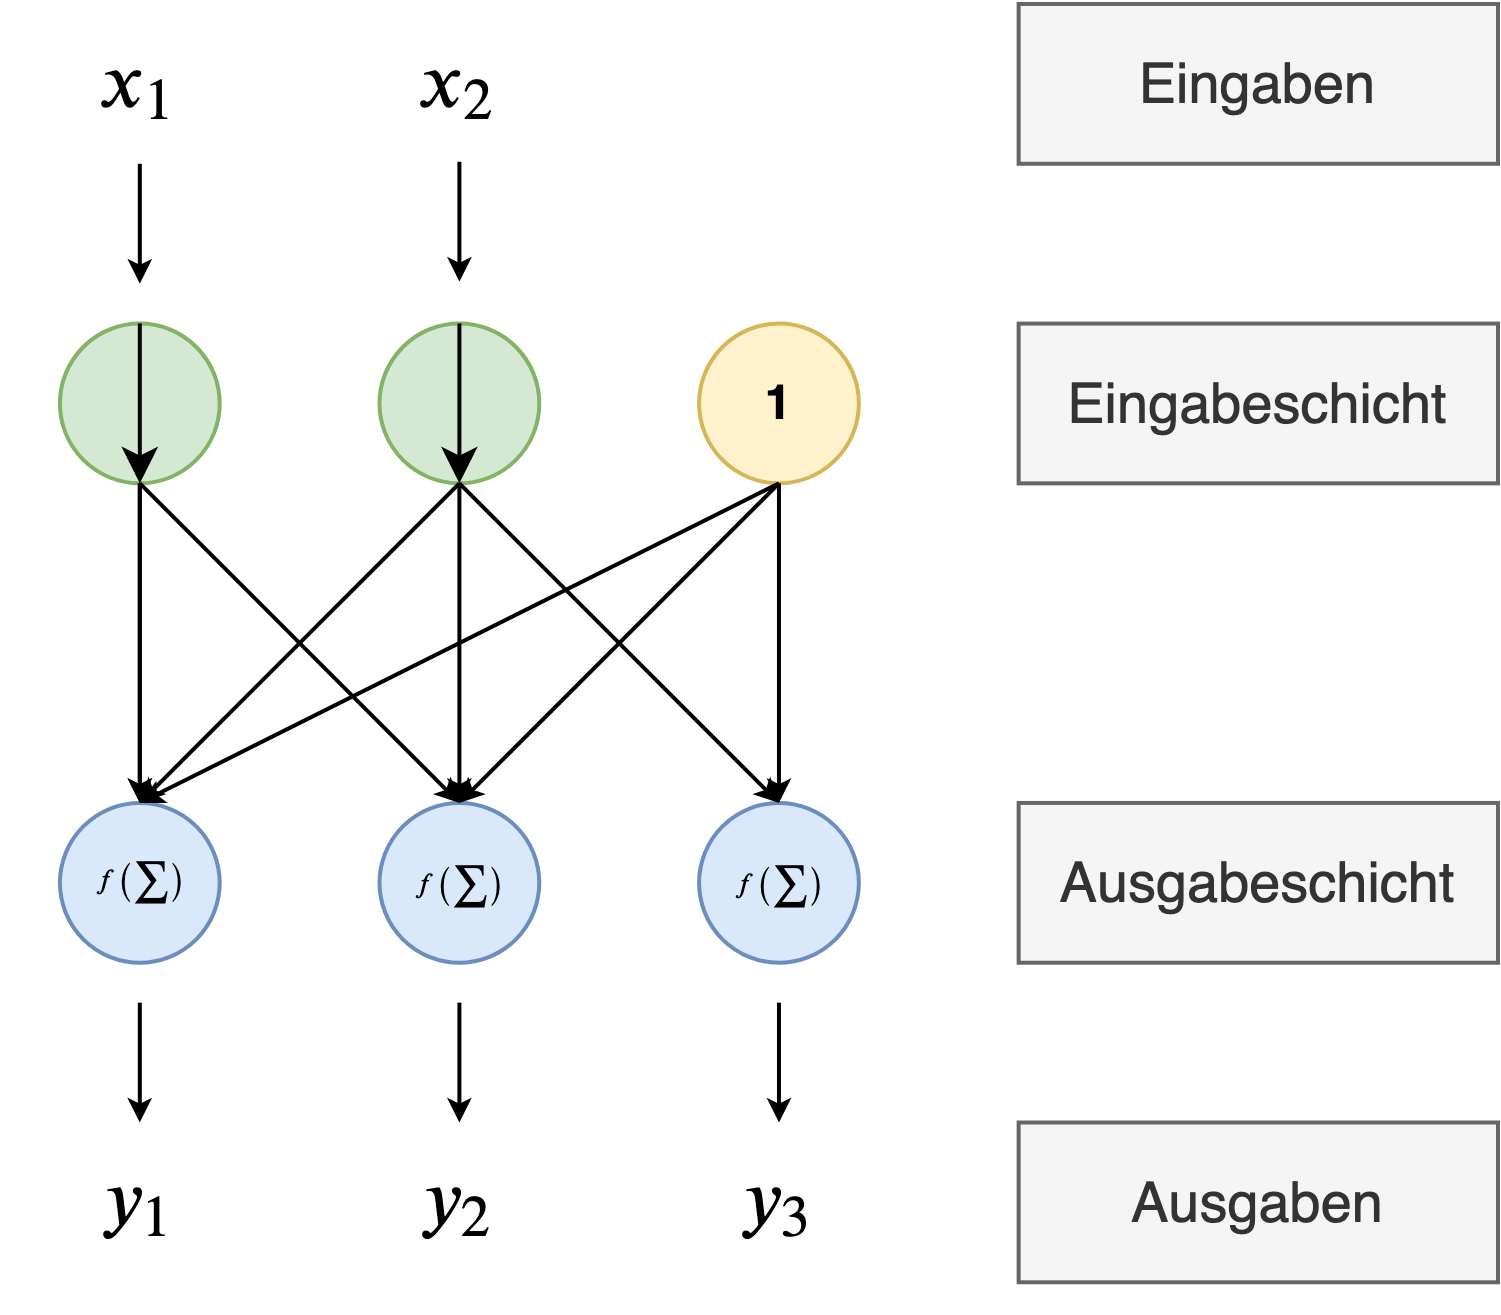
\includegraphics[width=0.7\textwidth]{multi_neuron_perceptron}
	\vspace*{-5mm}
	\caption[Einschichtiges Neuronales Netz]{Aufbau eines einschichtigen Neuronalen Netzes \cite[S.27]{BA}\cite[S.258]{MACHINE_LEARNING}.}
	\label{fig:multi_neuron_perceptron}
\end{figure}
\vspace*{-5mm}
Die Gewichtungen zwischen der Eingabeschicht und der Ausgabeschicht werden zur einfacheren Berechnung typischerweise als Matrix \textbf{W} dargestellt \eqref{eq:perzeptron_matrix} \cite[S.26]{BA}\cite[S.258]{MACHINE_LEARNING}.
\begin{equation}
\label{eq:perzeptron_matrix}
\begin{aligned}
\textbf{W} = 
\begin{pmatrix}
w_{11} & w_{12} & w_{13} \\
w_{21} & w_{22} & w_{23} \\
w_{b1} & w_{b2} & w_{b3} \\\end{pmatrix}
\end{aligned}
\end{equation}\myequations{Matrizendarstellung eines einschichtigen Neuronalen Netzes}\\ 
Mittels dieser Darstellung kann bei einer elementweisen Auswertung der Aktivierungsfunktion und einer Matrizenmultiplikation sehr einfach eine ähnliche Formel wie \eqref{eq:perceptron_def} angewandt werden, um die Ausgabe des Netzes zu errechnen:
\begin{equation}
\label{eq:slp_def}
\begin{aligned}
\textbf{y} = f_{akt}(\textbf{x}^T \cdot \textbf{W})
\end{aligned}
\end{equation}\myequations{Mathematische Definition eines einschichtigen Neuronalen Netzes}\\
Doch wie lernen einschichtige Neuronale Netze, sich an neue Informationen anzupassen? Früher und für nicht überwachtes Lernen wurde hier häufig die an die menschliche Biologie angelehnte Hebbsche Lernregel angewandt. Diese ist jedoch für überwachtes Lernen wie im Fall der Problemstellung eher ungeeignet. Es wird also das in der Praxis häufig eingesetzte Gradientenabstiegsverfahren betrachtet \cite[S.259]{MACHINE_LEARNING}. 
\subsubsection{Gradientenabstiegsverfahren} 
Die Idee hinter dem Gradientenabstiegsverfahren ist eine schrittweise Verringerung des Gesamtfehler eines einschichtigen Neuronalen Netzes \ensuremath{F} unter einer Fehlerfunktion \ensuremath{E(\textbf{y'}, \textbf{y})} für die Vorhersagen \ensuremath{\textbf{y'}} und die Labels \ensuremath{\textbf{y}}, indem eine optimale Kombination von Gewichten \ensuremath{\textbf{W}_{min}} gesucht wird \eqref{eq:gradient} \cite[S.28]{BA}.
\begin{equation}
\label{eq:gradient}
\begin{aligned}
\underset{\textbf{W}}{\text{min}} \medspace & & & F = E(f_{akt}(\textbf{x}^T \cdot \textbf{W}) ,y)
\end{aligned}
\end{equation}\myequations{Ziel des Gradientenabstiegsverfahren}\\
In einer dreidimensionalen Gebirgslandschaft, welche durch zwei Gewichte und den Fehler beschrieben ist, kann man sich die Arbeitsweise dieses Algorithmus leicht so vorstellen: Ein Bergsteiger mit eingeschränkter Sicht in dieser Landschaft kann sich lediglich über den Punkt des steilsten Abstiegs langsam und schrittweise in ein Tal wagen. Er versucht also immer weiter dem steilsten Abstieg zu folgen, bis er ein Tal der Fehlerfunktion findet. Dies lässt sich in \ref{fig:gradient} erkennen \cite[S.28]{BA}\cite[S.39]{NN}. 
\begin{figure}[H]
	\centering
	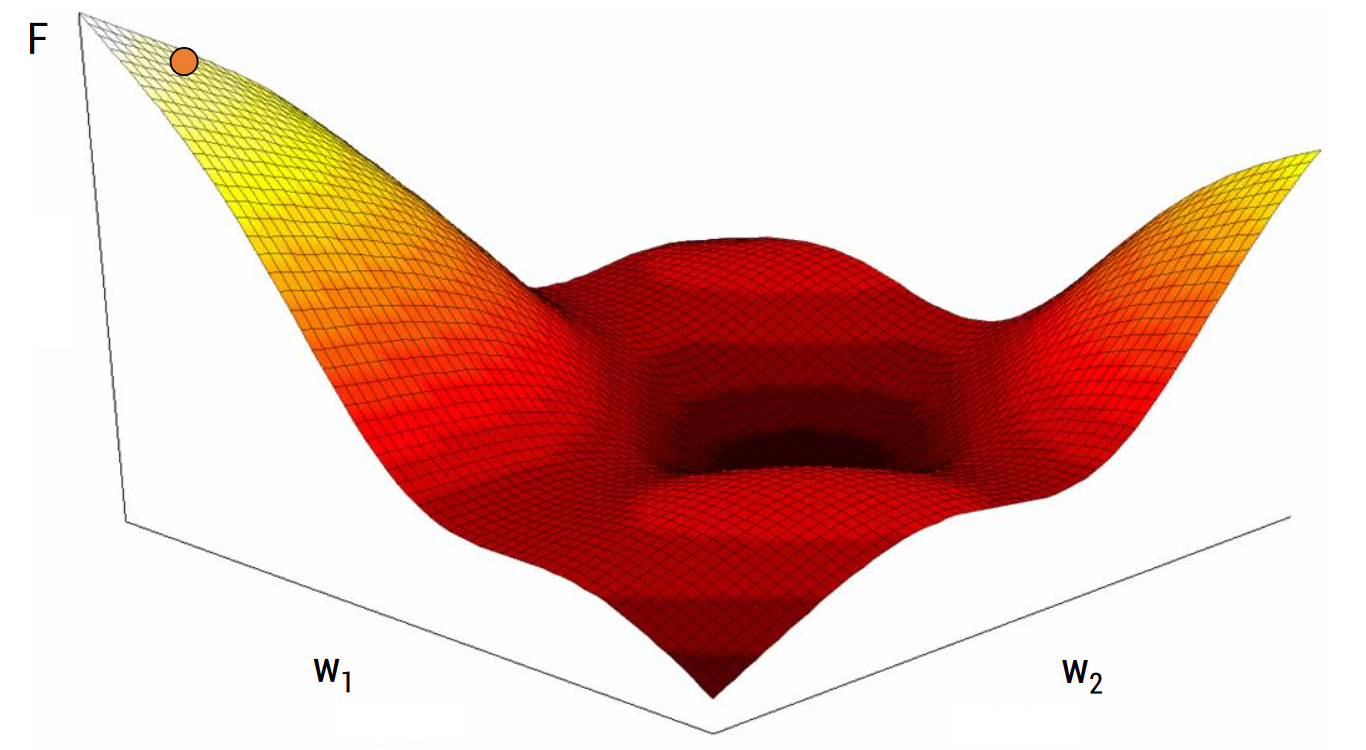
\includegraphics[width=1.0\textwidth]{gradient}
	\vspace*{-5mm}
	\caption[Fehler im Neuronalen Netz]{Gebirgslandschaft des Fehlers in einem Neuronalen Netz \cite{GRADIENT_IMAGE}.}
	\label{fig:gradient}
\end{figure}
Im Algorithmus funktioniert dies durch partielle Ableitungen der Fehlerfunktion nach jedem Gewicht und einem Anwenden des daraus resultierenden Gradientenvektors in negativer Richtung angepasst durch die gewählte Lernrate, welche die Geschwindigkeit des Abstiegs zum Minimum definiert. Dies wird wiederholt, bis ein gewünschtes Minimum oder eine gewählte Zahl an Wiederholungen erreicht wurde. Die Wiederholungen werden bei Neuronalen Netzen über alle Trainingsdaten auch als Epochen bezeichnet \cite[S.29-30]{BA}\cite[S.41]{NN}\cite[S.31]{DEEP_LEARNING}. Häufig wird jede Epoche aber auch noch in kleinere Teile, die sogenannten Batches, unterteilt.
\begin{figure}[H]
	\centering
	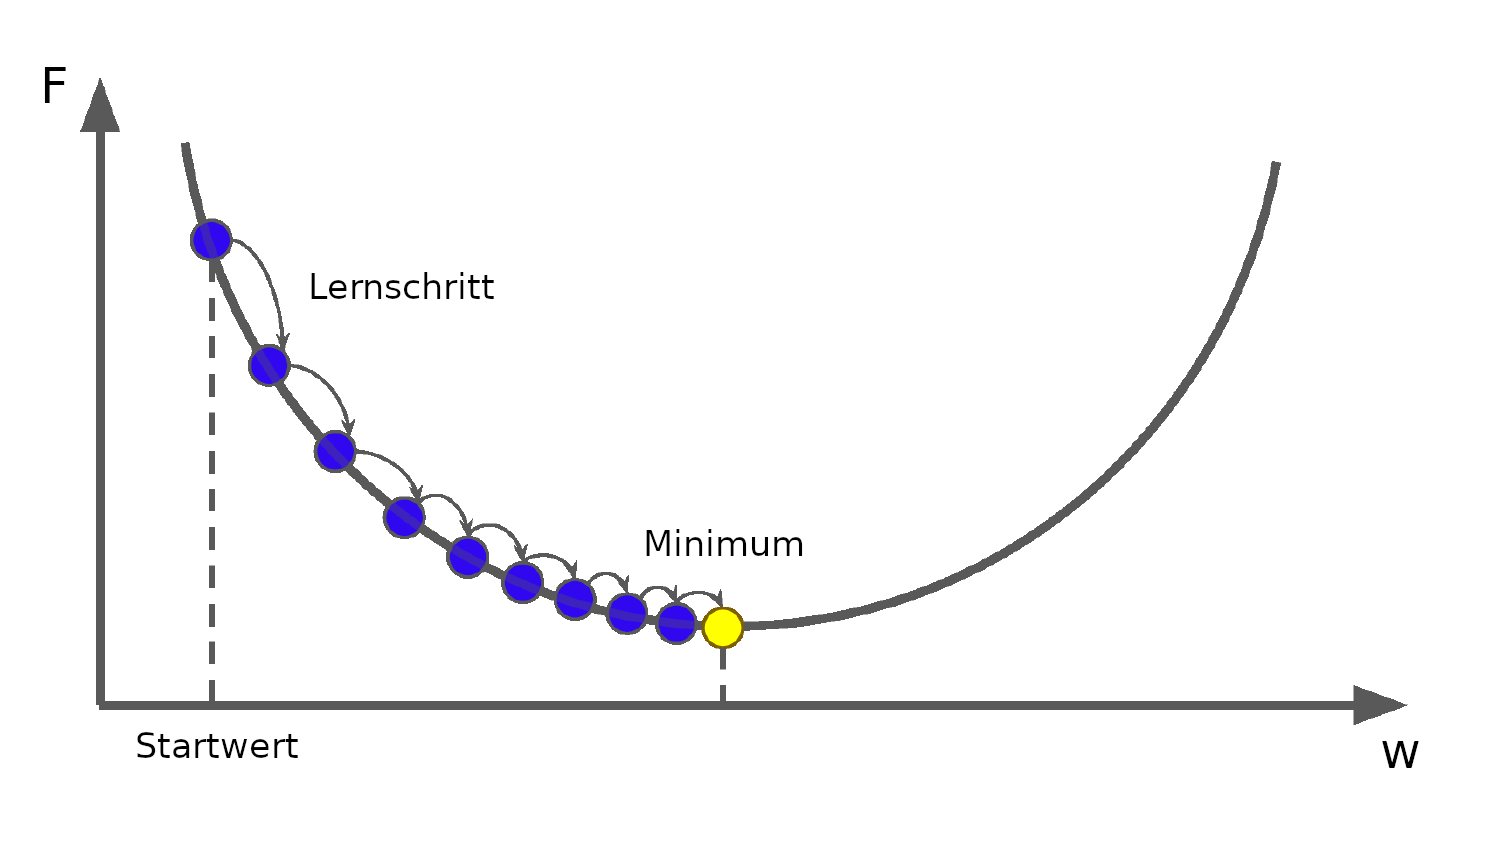
\includegraphics[width=0.8\textwidth]{2DGradient}
	\vspace*{-5mm}
	\caption[Gradientenabstiegsverfahren in zwei Dimensionen]{Das Gradientenabstiegsverfahren in zwei Dimensionen \cite[S.113]{MACHINE_LEARNING}.}
	\label{fig:2DGrad}
\end{figure}
\vspace*{-5mm}
Bereits durch die Beschreibung des Algorithmus lassen sich einige Probleme abschätzen. Zum einen ist nicht gewährleistet, dass ein globales Minimum gefunden wird. Stoppt der Algorithmus in einem lokalen Minimum, so kann nicht weiter optimiert werden. Eine höhere Lernrate oder ein Momentum-Term, welcher dem Algorithmus beim Durchlaufen der mehrdimensionalen Gebirgslandschaft eine gewisse Trägheit gibt, können dafür sorgen, dass lokale Minima übersprungen werden. Eine hohe Lernrate kann aber auch zu Problemen führen. So ist in diesem Fall eine ein- oder mehrschrittige Oszillation zwischen den Talrändern ein typisches Problem, welches auftreten kann. Auch kann sie zum Überspringen des globalen Minimum führen \cite[S.30]{BA}\cite[S.46-47]{NN}.
\\\\
Ein weiteres Problem tritt bezüglich der bisher bekannten Aktivierungsfunktion, der Schwellenwertfunktion, auf. Für diese kann kein Gradient ungleich null berechnet werden, wodurch kein Minimum gefunden werden kann. Dies kann durch das Einführen anderer Aktivierungsfunktionen gelöst werden und wird in einem späteren Kapitel betrachtet \cite[S.31-32]{BA}\cite[S.262]{MACHINE_LEARNING}.
\subsubsection{Mehrschichtige Neuronale Netze}
Leider lassen sich mit einschichtigen Neuronalen Netzen nur einfache Probleme lösen. Dies lässt sich durch das Einfügen weiterer Schichten lösen, indem die Ausgaben der vorherigen Schicht durch weitere erlernbare Gewichtungen an die nächste Schicht weitergegeben werden. Alle Schichten zwischen der Eingabe- und Ausgabeschicht werden dabei als verborgene Schichten oder Hidden-Layer bezeichnet \cite[S.31-32]{BA}\cite[S.261]{MACHINE_LEARNING}. Ein Beispiel hierfür ist in der folgenden Abbildung zu erkennen: 
\begin{figure}[H]
	\centering
	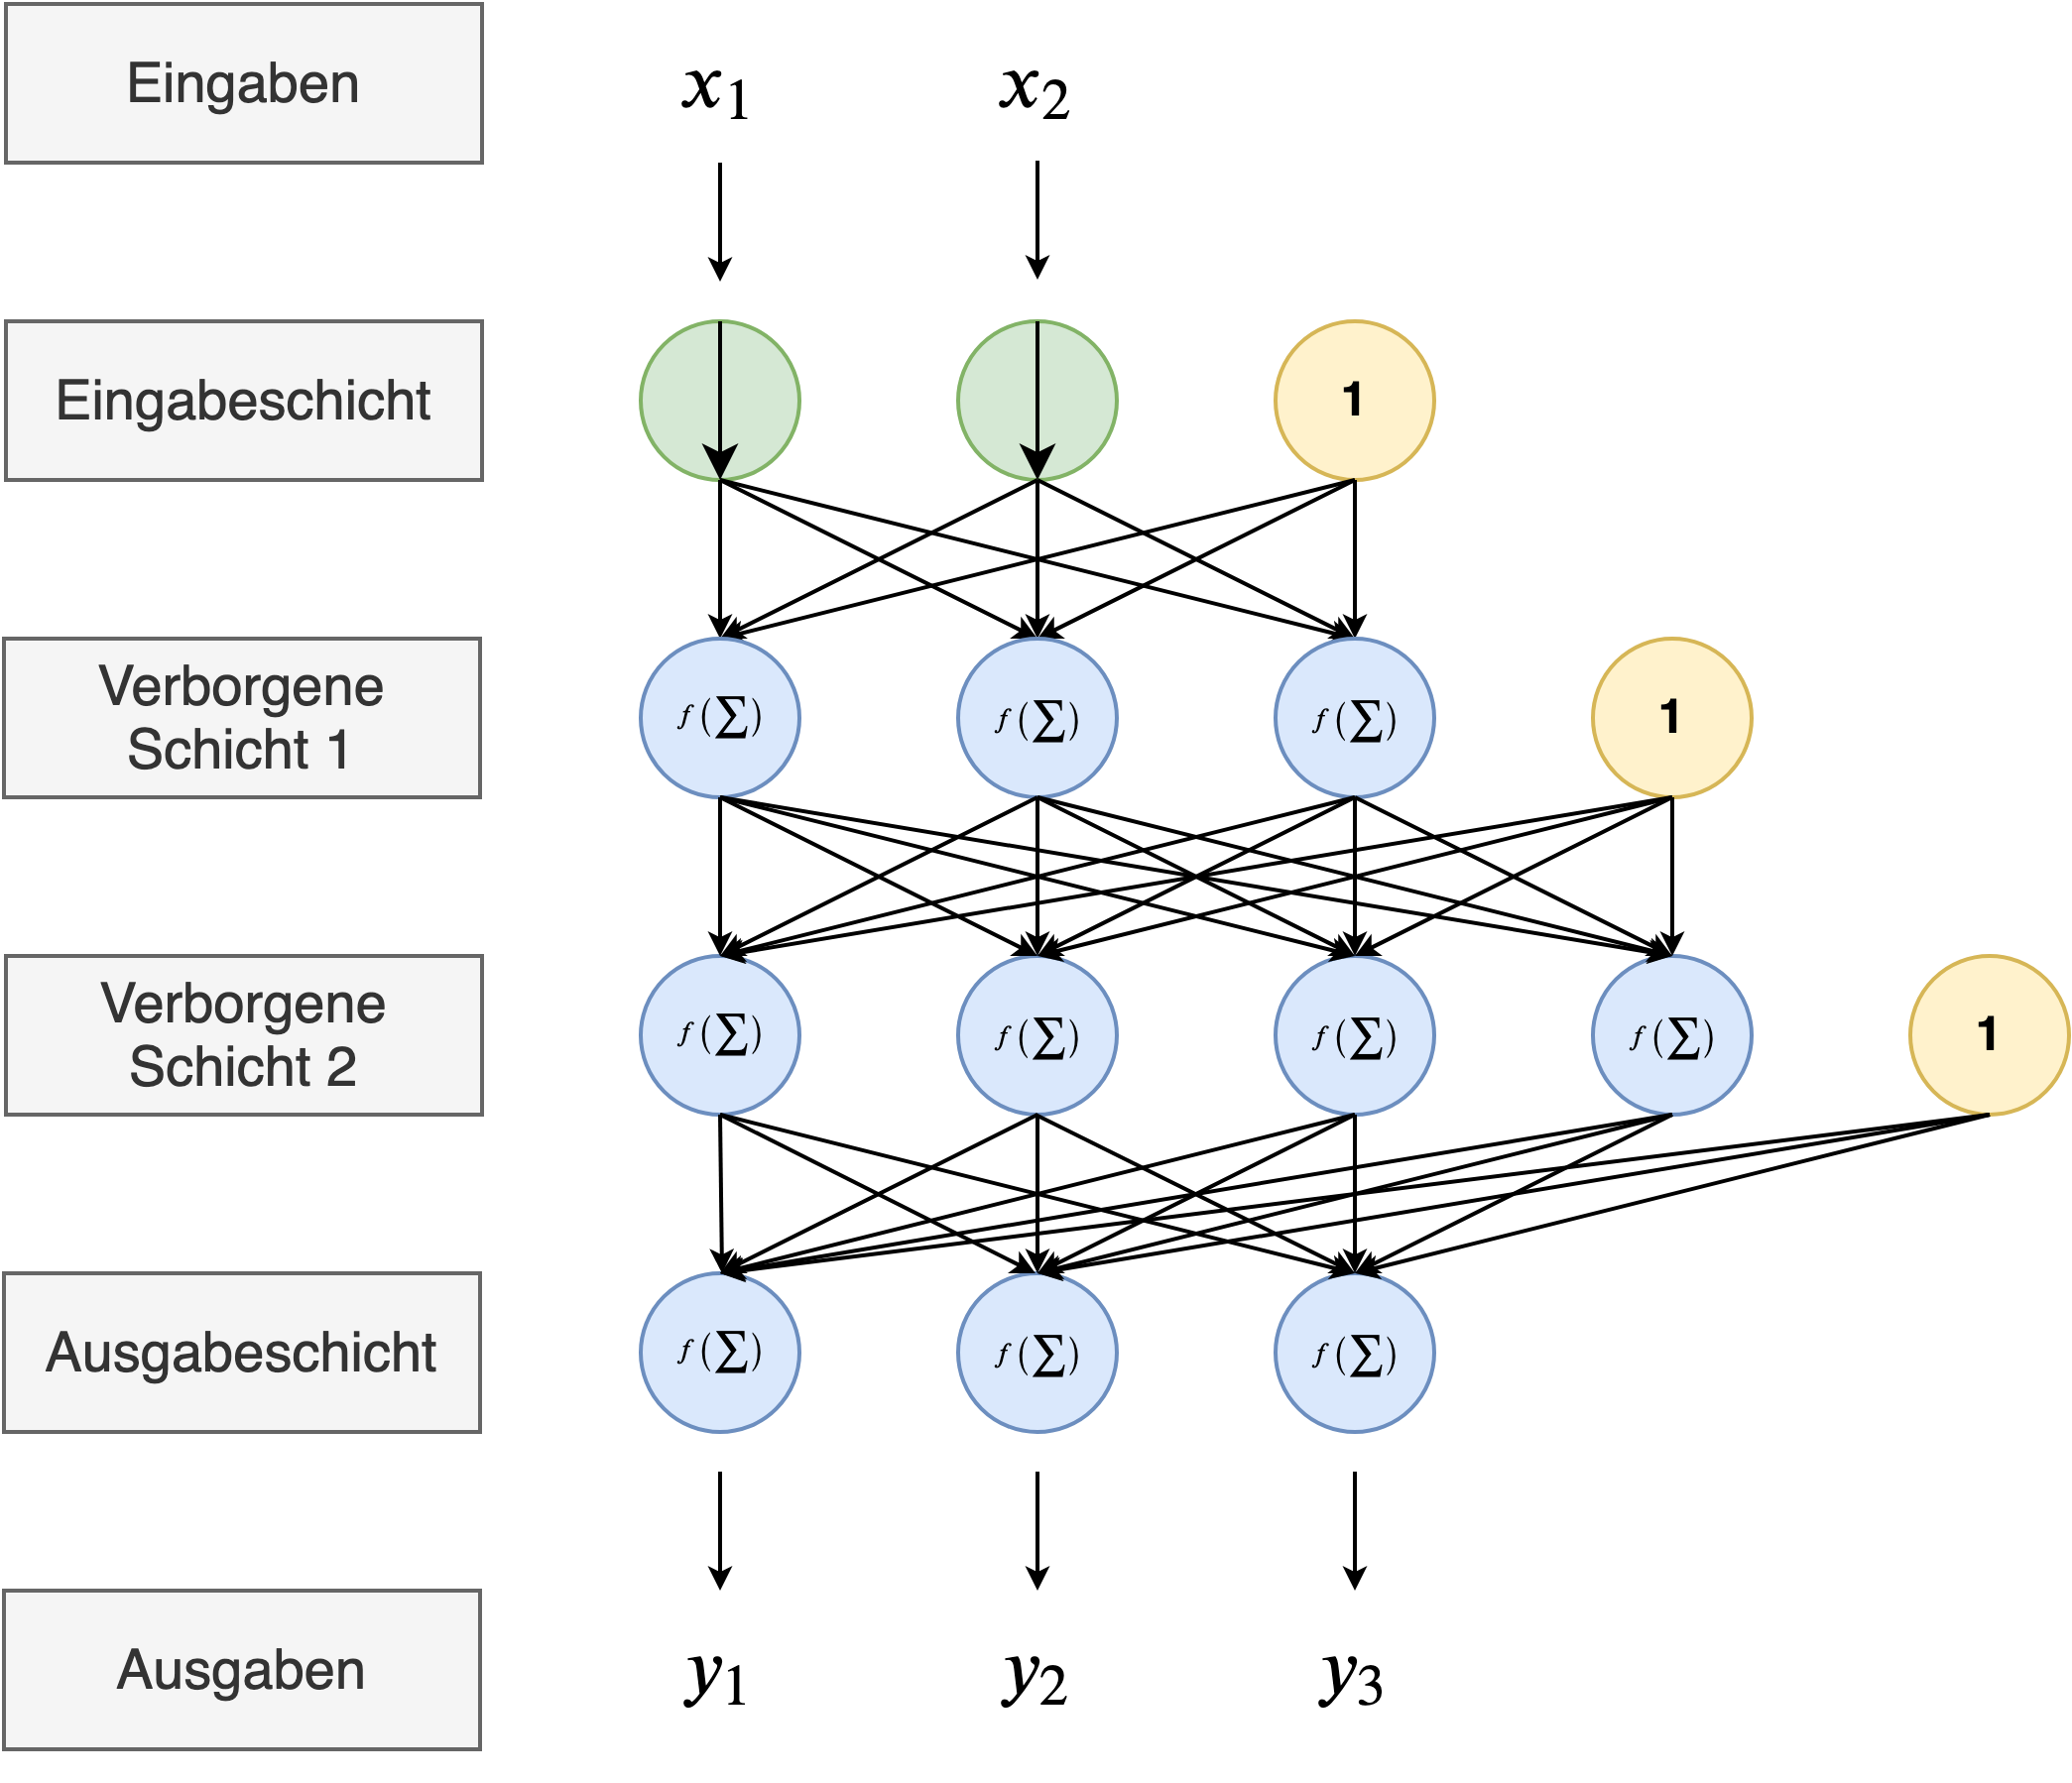
\includegraphics[width=0.85\textwidth]{multi_layer_perceptron}
	\vspace*{-3mm}
	\caption[Mehrschichtiges Neuronales Netz]{Ein mehrschichtiges Neuronales Netz mit zwei verborgenen Schichten \cite[S.32]{BA}\cite[S.261]{MACHINE_LEARNING}.}
	\label{fig:mutlilayer_nn}
\end{figure}
\vspace*{-5mm}
Leider funktioniert das Gradientenabstiegsverfahren in der bisherigen Funktionsweise nur mit einem einzigen Layer, da der Fehler von verborgenen Schichten nicht direkt errechnet werden kann. Es fehlt damit eine Lernmethode für das überwachte Lernen. Die Lösung hierfür ist das Backpropagation-Verfahren \cite[S.261]{MACHINE_LEARNING}. 
\subsubsection{Backpropagation-Verfahren}
Über das Backpropagation-Verfahren wird der Fehler eines mehrschichtigen Neuronalen Netzes über seine Schichten zurückgerechnet, um eine Veränderungen der Gewichtungen in den verborgenen Schichten zu ermöglichen \cite[S.51-52]{NN}.
\\\\
Das Backpropagation-Verfahren wird folgendermaßen ausgeführt: Nachdem die Netzausgabe bestimmt wurde, wird für diese der Fehler zu den gewünschten Ausgaben errechnet. In der Ausgabeschicht wird mit dem Gradientenabstiegsverfahren für jedes Gewicht der negative Gradient zum letzten Hidden-Layer errechnet. Dieser wird nun durch die Gewichte der verbundenen Hidden-Neuronen zurückgerechnet und damit auf diese verbundenen Hidden-Neuronen verteilt. Wird dies für alle Neuronen der betrachteten Schicht wiederholt, kann mittels des Gradientenabstiegsverfahren der Fehler der verbundenen verborgenen Schicht errechnet werden. Dies wird wiederholt, bis die Eingabeschicht erreicht wurde \cite[S.33]{BA}\cite[S.52-53]{NN}. Wurden die Gradienten errechnet, können die Gewichtungen mit einem vorher definierten Lernparameter angepasst werden \cite[S.262]{MACHINE_LEARNING}. Der Algorithmus wird nun batch- und epochenweise solange wiederholt, bis der Fehler ein Limit unterschreitet oder eine maximale Anzahl an Wiederholungen erreicht wurde \cite[S.52]{NN}.
\\\\
Typischerweise können bei dem Backpropagation-Verfahren ähnliche Probleme wie beim Gradientenabstiegsverfahren auftreten. Außerdem können Gradienten aufgrund des Zurückrechnens sehr klein ausfallen und zu einer immer kleiner werdenden Anpassung der Gewichte in den ersten Schichten führen. Dies würde zu einem immer kleiner werdenden Lerneffekt führen. In wenigen Fällen kann auch ein gegenteiliges Problem, nämlich explodierende Gradienten, auftreten \cite[S.33-34]{BA}\cite[S.275-276]{MACHINE_LEARNING}. In der Regel lässt sich dies über sinnvoll ausgewählte Aktivierungsfunktionen und spezielle Regularisierungsverfahren lösen, die in den nächsten Kapiteln betrachtet werden. 
\subsubsection{Aktivierungsfunktionen}
Moderne Neuronale Netze verwenden in der Regel Aktivierungsfunktionen, welche auf der ReLU (Rectified Linear Units) basieren. Die ReLU hat im Gegensatz zu anderen, typischerweise früher eingesetzten Aktivierungsfunktionen wie der Sigmoidfunktion oder dem Tangens hyperbolicus, den Vorteil, dass sie keinen Sättigungseffekt durch eine sehr kleine Ableitung für positive Werte erfährt. Dies wirkt dem Problem der schwindenden Gradienten entgegen \cite[S.34-35]{BA}. Für die Eingabe x ist die ReLU definiert als \cite[S.245, S.279]{MACHINE_LEARNING}:
\begin{equation}
\label{eq:relu}
\begin{aligned}
f_{akt} =
\begin{cases}
x & x \geq 0\\
0 & x < 0
\end{cases}
\end{aligned}
\end{equation}\myequations{ReLU}\\
Wie zu sehen ist, ist die ReLU für positive Werte lediglich äquivalent zu der originalen Eingabe. Damit ist sie sehr einfach zu berechnen. Leider leidet sie unter einem großen Problem: Ein Neuron mit einer negativen Eingabesumme vor der Aktivierungsfunktion liefert eine Konstante 0 und trägt nicht mehr zum Lernen bei. Tritt dies bei vielen Neuronen auf, kann dies ebenfalls den Lerneffekt beschränken \cite[S.279]{MACHINE_LEARNING}.
\\\\
In vielen Fällen wird dies über die Verwendung leicht abgewandelter ReLU-Varianten wie der Leaky-ReLU oder der ELU (Exponential Linear Unit), die auch in diesem Projekt verwendet wurde, gelöst. Die ELU hat im Positiven ein lineares Verhalten, während sie sich im negativen Bereich wie eine Exponentialfunktion im Negativen verhält, die sich einem Parameter a annähert. Es gilt \cite[S.36]{BA}:
\begin{equation}
\label{eq:elu}
\begin{aligned}
f_{akt} =
\begin{cases}
x & x \geq 0\\
a(e^x - 1) & x < 0
\end{cases}
\end{aligned}
\end{equation}\myequations{ELU}\\
Mit diesen Aktivierungsfunktionen können bereits einige typische Probleme beim Maschinellen Lernen mit mehrschichtigen Neuronalen Netzen und Backpropagation verhindert werden. Eine weitere verwendete Aktivierungsfunktion, welche vor allem bei der Ausgabeschicht von Klassifikationsproblemen mit One-Hot kodierten Labeln nützlich ist, ist die Softmax-Funktion. Im Gegensatz zu anderen Aktivierungsfunktionen erhält sie die Ausgabe aller Neuronen einer Schicht. Diese Ausgaben werden dann mit der Summe aller Ausgaben normalisiert, was in einem Vektor von Zahlen zwischen 0 und 1 resultiert. Diese werden in der Regel als Wahrscheinlichkeiten für eine vorliegende Klasse interpretiert. Für den Vektor mit Neuronensummen \ensuremath{\textbf{s}} mit n-Elementen ist die Softmax definiert als \cite[S.37]{BA}\cite[S.141-142, S.263]{MACHINE_LEARNING}: 
\begin{equation}
\label{eq:softmax}
\begin{aligned}
f_{akt} = \frac{e^{s_i}}{\sum_{i=1}^{n}e^{s_i}}
\end{aligned}
\end{equation}\myequations{Softmax}
\subsubsection{Regularisierungsverfahren}
Zuletzt werden nun zwei typische Regularisierungsverfahren für Neuronale Netze betrachtet, mit denen deren Performanz auf bestimmte Weisen erhöht werden kann.
\\\\
Die Batch-Normalisierung ist ein ideales Verfahren, um schwindenden Gradienten sowie Overfitting entgegenzuwirken und die Stabilität von Neuronalen Netzen zu erhöhen. Diese wird schicht- und batchweise ausgeführt, indem die Summe aller Neuronen einer Schicht vor der Aktivierungsfunktion standardisiert wird. Das Verfahren arbeitet, indem der Mittelwert auf 0 zentriert und durch die Standardabweichung der Batch geteilt wird. Dann wird das Ergebnis über zwei lernbare Parameter skaliert und verschoben. Dadurch kann das Netz die ideale Skalierung und den Mittelwert der Eingaben für eine Schicht erlernen. Schwindende Gradienten werden dadurch so stark bekämpft, dass sogar der Einsatz der Sigmoidfunktion oder des Tangens hyperbolicus wieder denkbar wäre \cite[S.37-38]{BA}\cite[S.282-283]{MACHINE_LEARNING}.
\\\\
Eine weitere Möglichkeit zur Regularisierung ist ein Dropout in verborgenen Schichten. Das Prinzip vom Dropout ist, dass Neuronen in einer Schicht während eines Schritts des Trainingsvorgangs mit einer gewissen Wahrscheinlichkeit ausgelassen werden. Wird der nächste Schritt erreicht, so werden die Dropouts neu ausgewürfelt. Durch das Auslassen von gewissen Neuronen werden andere dazu gezwungen, ihr Wissen zu verallgemeinern, da sie sich nicht auf die ausgeschiedenen Neuronen verlassen können. Dies wirkt Overfitting entgegen \cite[S.38-39]{BA}\cite[S.205-206]{NNP}.
\subsection{Konvolutionelle Neuronale Netze}
Heutzutage werden für Aufgaben der Bilderkennung in der Regel keine einfachen Neuronalen Netze, sondern Konvolutionelle Neuronale Netze eingesetzt. Diese wurden zum ersten mal 1980 eingesetzt und sind am Aufbau des visuellen Cortex des Menschen angelehnt. In diesem Arbeiten Neuronen in verschiedenen Schichten von Filtern, die aufeinander aufbauen. Die oberen Filter erkennen viele einfache Bildelemente, wie unterschiedliche Ausrichtungen von Linien. Diese werden weiter an untere Schichten geleitet, die das gefilterte immer weiter zu komplexen Mustern und Bildern kombinieren können \cite[S.360]{MACHINE_LEARNING}. 
\begin{figure}[H]
	\centering
	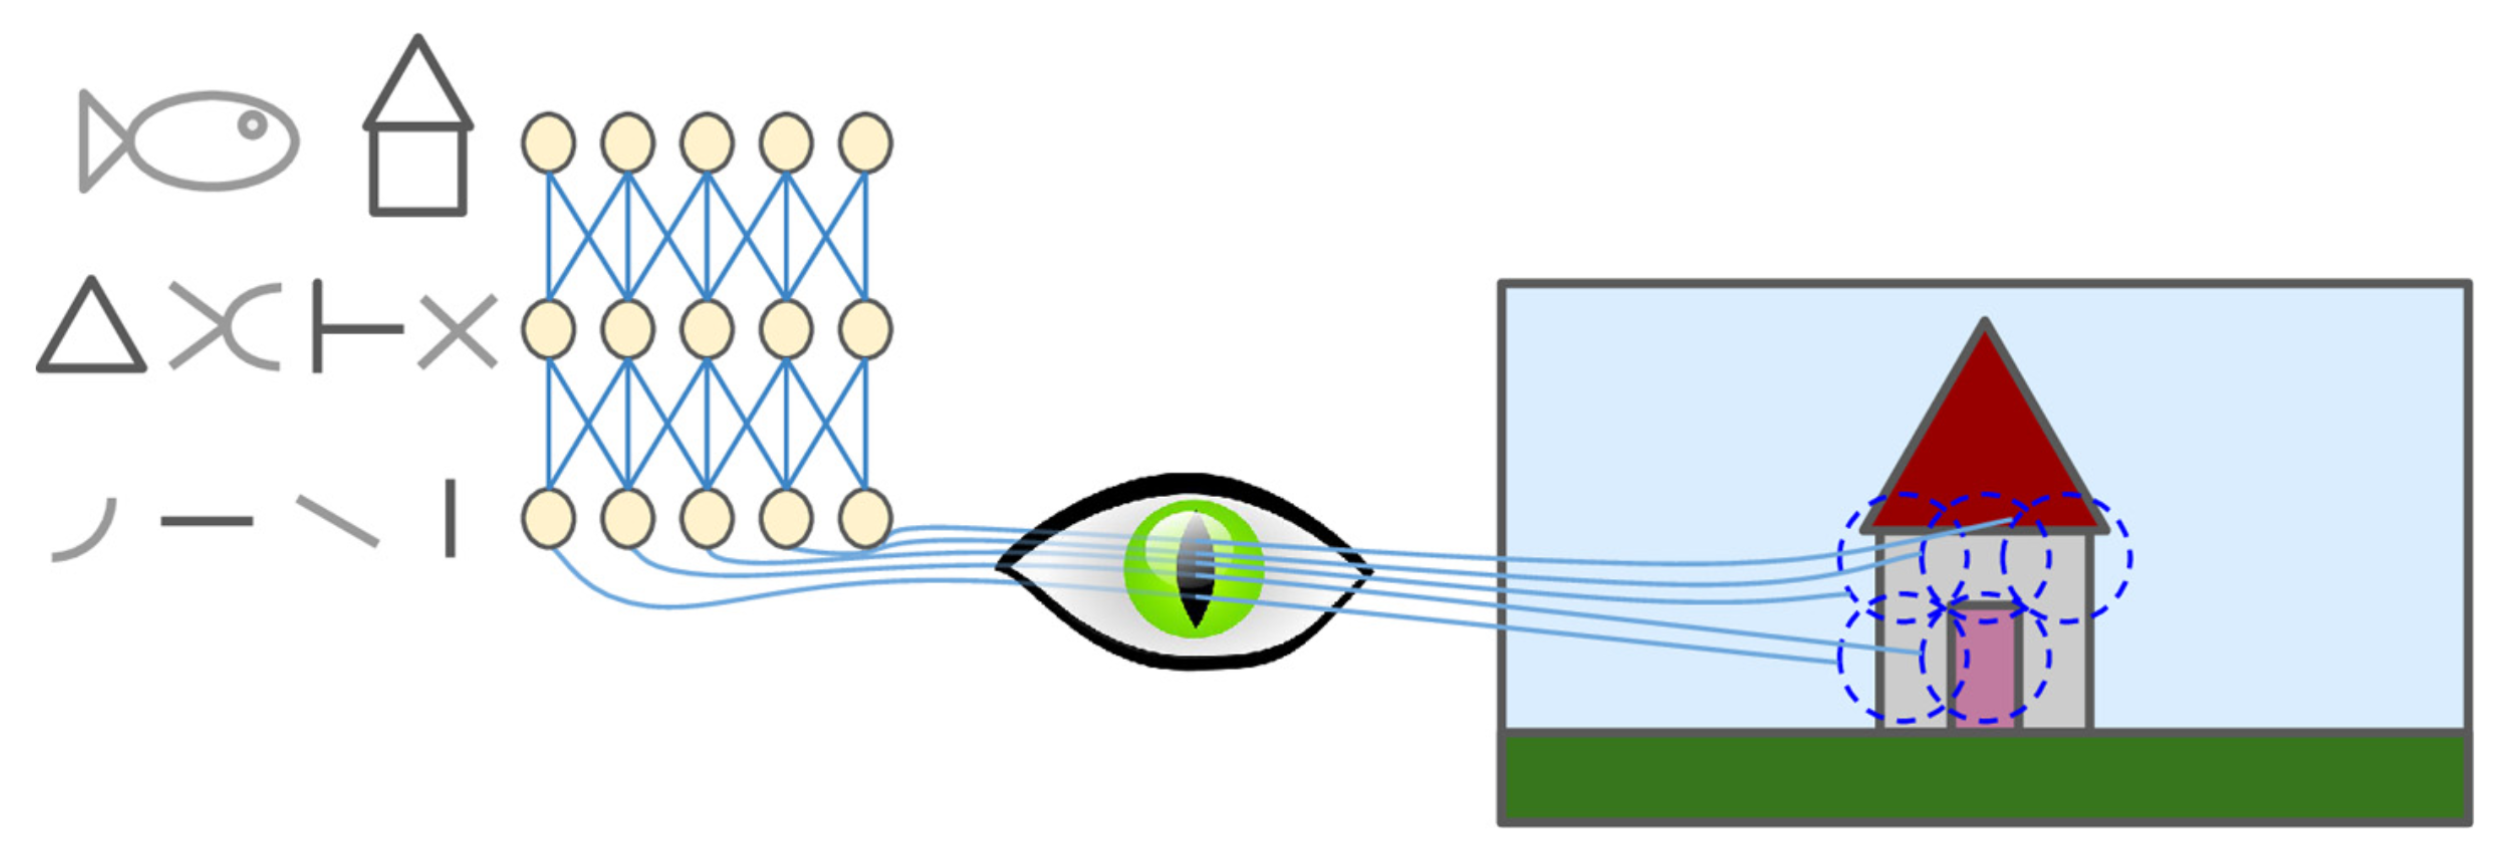
\includegraphics[width=0.85\textwidth]{visueller_cortex}
	\vspace*{-3mm}
	\caption[Aufbau des visuellen Cortex]{Aufbau des visuellen Cortex eines Menschen \cite[S.360]{MACHINE_LEARNING}.}
	\label{fig:visueller_cortex}
\end{figure}
\vspace*{-5mm}
Diese Erkenntnisse wurden dann genutzt, um 1980 die ersten Konvolutionelle Neuronale Netze zu entwickeln und für die Erkennung von handgeschriebenen Ziffern zu nutzen. Ein typischer Aufbau für Konvolutionelle Neuronale Netze besteht aus drei verschiedenen Schichten. Die letzten Schichten sind dabei in der Regel die bereits betrachteten vollständig verbundenen Neuronale Netz Schichten. Am Anfang befinden sich allerdings im Wechsel Convolutional und Pooling Layer, welche im folgenden betrachtet werden \cite[S.361]{MACHINE_LEARNING}.
\subsubsection{Convolutional Layer}
Convolutional Layer bestehen vom Grundprinzip aus einer zweidimensionalen Gewichtsmatrix von Neuronen einer gewissen Höhe und Breite, auch Filter genannt, welche mit einer bestimmten Schrittweite (Stride) über ein Eingabebild- oder ein bereits vorher durch einen Convolutional Layer betrachtetes Bild wandern. Der Filter multipliziert dabei in jedem durch die Schrittweite betrachtete Ausschnitt des Bildes, die Bildpunkte mit eigenen im Filter vorhandenen und lernbaren Gewichtungen. Dann werden die gewichteten Bildpunkte aufsummiert. Es entsteht ein neuer Bildpunkt, welcher wenn ein zum Filter passendes Feature betrachtet wurde, einen hohen Wert aufweisen wird. Damit Randpixel betrachtet werden können, muss abhängig von der Filtergröße ein Padding am Rand des Bildes hinzugefügt werden. Hier sind unterschiedliche Arten wie ein Zero-Padding, also ein Auffüllen des Rands mit Nullen, denkbar. In der Abbildung \ref{fig:cnn_filter} ist ein Convolutional Layer mit einer Filtergröße von 3x3 Pixeln, einer Schrittweite von 2 und ein Zero-Padding erkennbar. Bei dieser Schrittweise ist klar zu erkennen, dass das Bild durch diese verkleinert wird. Dies ist nützlich, da hierdurch Bildauflösungen verringert werden können \cite[S.361-363]{MACHINE_LEARNING}.
\begin{figure}[H]
	\centering
	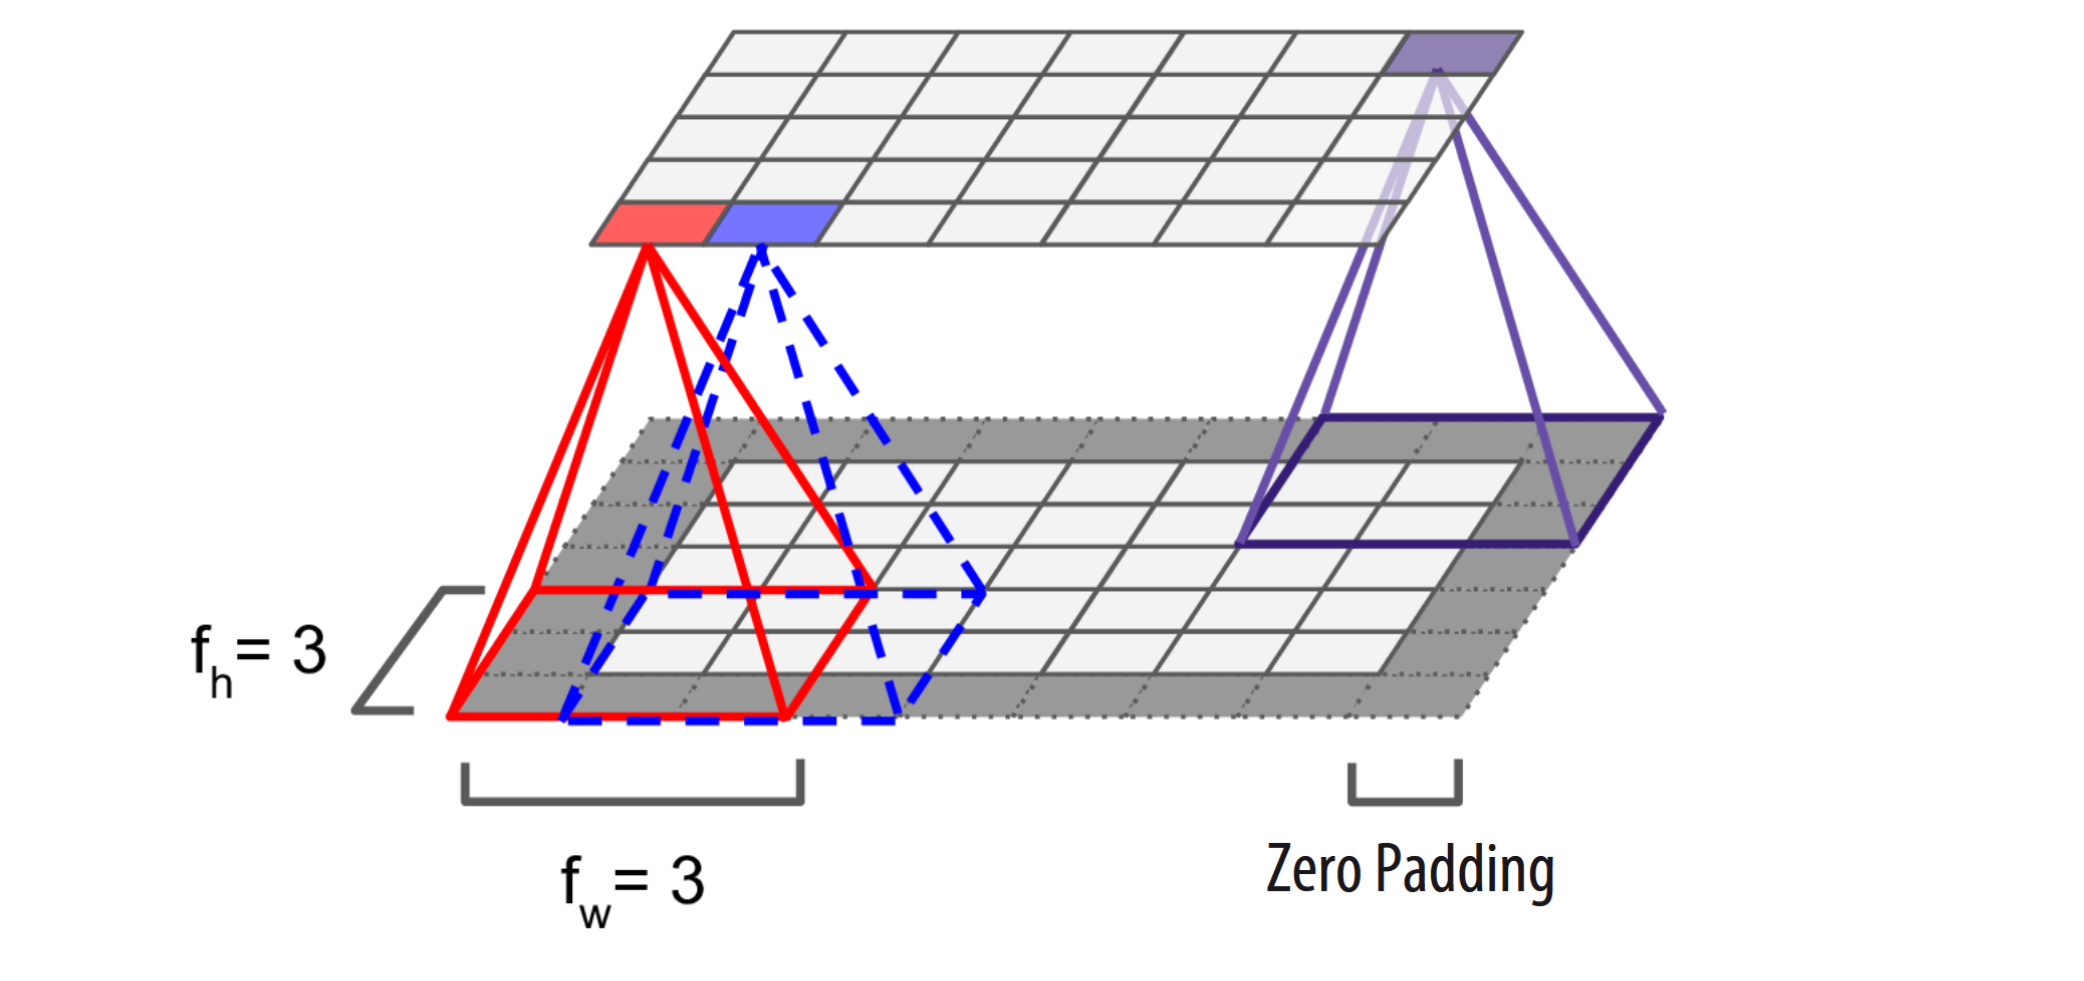
\includegraphics[width=0.85\textwidth]{cnn}
	\vspace*{-3mm}
	\caption[Einzelner Filter eines Convolutional Layers]{Ein einzelner Filter eines Convolutional Layers \cite[S.362]{MACHINE_LEARNING}.}
	\label{fig:cnn_filter}
\end{figure}
\vspace*{-5mm}
Die Arbeitsweise eines Filters ist sehr einfach zu visualisieren. Ein Filter, welcher in einer einzelnen Linie in einer vertikalen Ausrichtung hohe Gewichtungen aufweist, würde in einem Bild vertikale Linie hervorheben und horizontale Linie verschwimmen lassen. Demgegenüber würde ein horizontaler Linienfilter, horizontale Linien hervorheben und vertikale verschwimmen lassen \cite[S.363-364]{MACHINE_LEARNING}. Ein Beispiel hierfür ist in folgender Abbildung zu erkennen:
\begin{figure}[H]
	\centering
	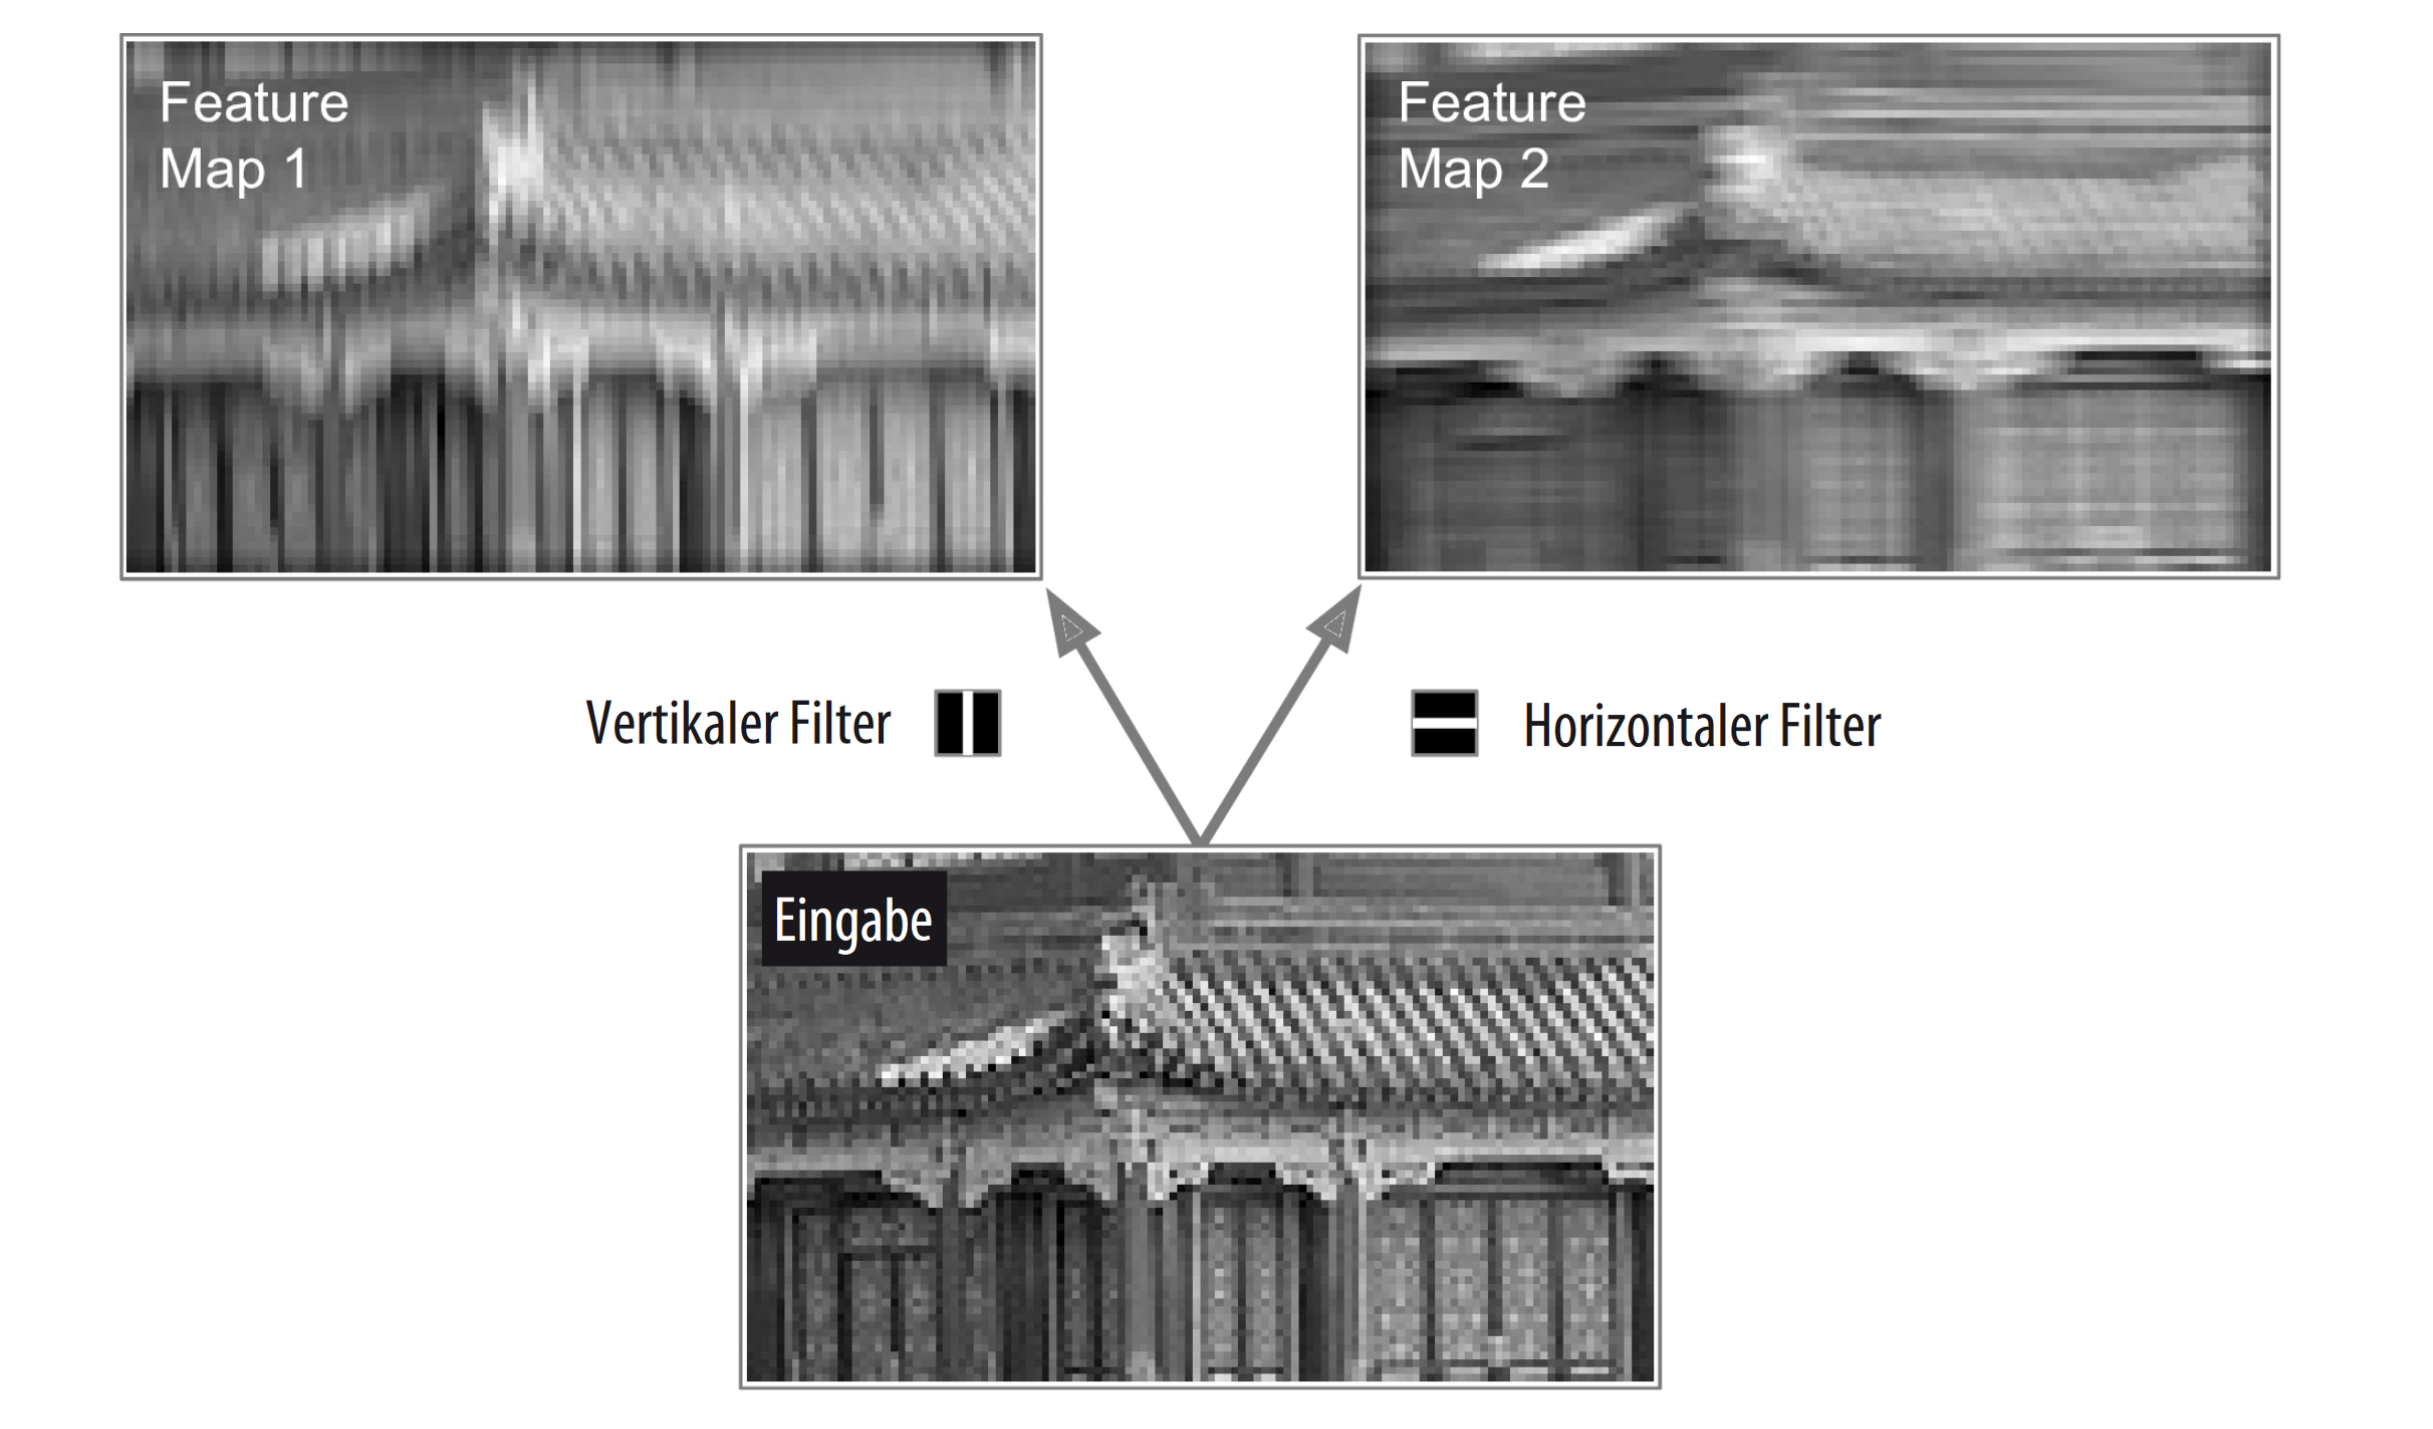
\includegraphics[width=0.85\textwidth]{filter_example}
	\vspace*{-3mm}
	\caption[Beispiel für horizontale und vertikale Filter]{Ein Beispiel für horizontale und vertikale Filter \cite[S.364]{MACHINE_LEARNING}.}
	\label{fig:cnn_filter_example}
\end{figure}
\vspace*{-5mm}
In der Abbildung \ref{fig:cnn_filter_example_2} ist außerdem ein typisches Beispiel für visualisierte Filter des ersten Convolutional Layers in einem CNN zu erkennen. Es wird klar ersichtlich, dass die dargestellten Filter verschiedene Strukturen erkennen können \cite[S.132]{DEEP_LEARNING_REVOLUTION}.
\begin{figure}[H]
	\centering
	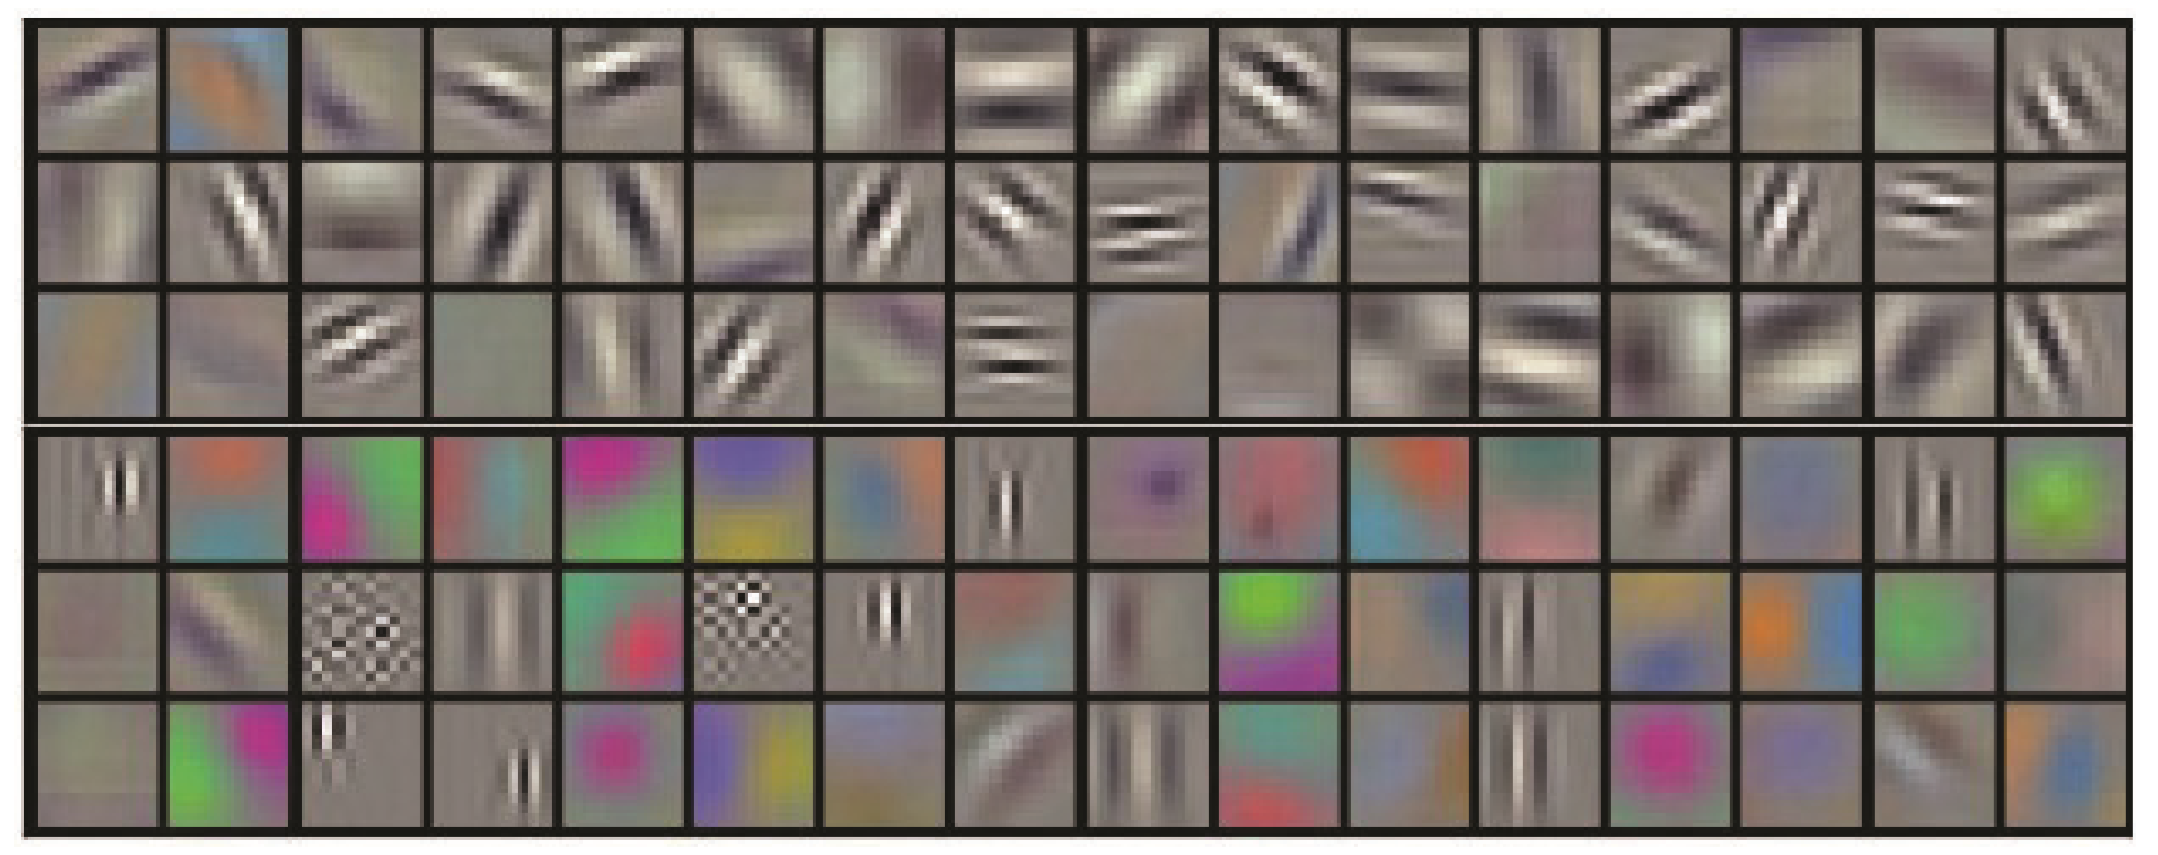
\includegraphics[width=0.85\textwidth]{cnn_filter}
	\vspace*{-3mm}
	\caption[Beispiel für verschiedene visualisierte Filter]{Ein Beispiel für verschiedene visualisierte Filter im ersten Convolutional Layers eines CNNs \cite[S.132]{DEEP_LEARNING_REVOLUTION}.}
	\label{fig:cnn_filter_example_2}
\end{figure}
\vspace*{-5mm} 
Wie in der Abbildung zu sehen, gibt es pro Convolutional Layer gleich mehrere Filter, die sogar Farben verarbeiten können. Zwar lassen sich mit mehreren bisher beschriebenen Filtern pro Convolutional Layer auch schon mehrere Features von Grauwertbildern (ein Grauwert pro Bildpunkt) sehr gut extrahieren, jedoch gehen so viele Bildinformationen der Farbe verloren, deshalb sind tatsächliche Filter in modernen CNNs eher dreidimensionale Matrizen. Die Höhe und Breite dieser ist weiterhin die selbe definierte Größe wie bei bisher bekannten Filtern, jedoch weisen sie in der Tiefe weitere Reihen von Filtern auf. Diese können Informationen aus den Farbkanälen extrahieren. Weiterhin können pro Convolutional Layer wie in der Abbildung zu sehen war, mehrere Filter eingesetzt werden. Daraus resultiert ein Stapel sogenannter Feature Maps auf denen erneut ein dreidimensionaler Filter angewandt werden kann \cite[S.364-365]{MACHINE_LEARNING}. Dies ist in folgender Abbildung gut zu erkennen:
\begin{figure}[H]
	\centering
	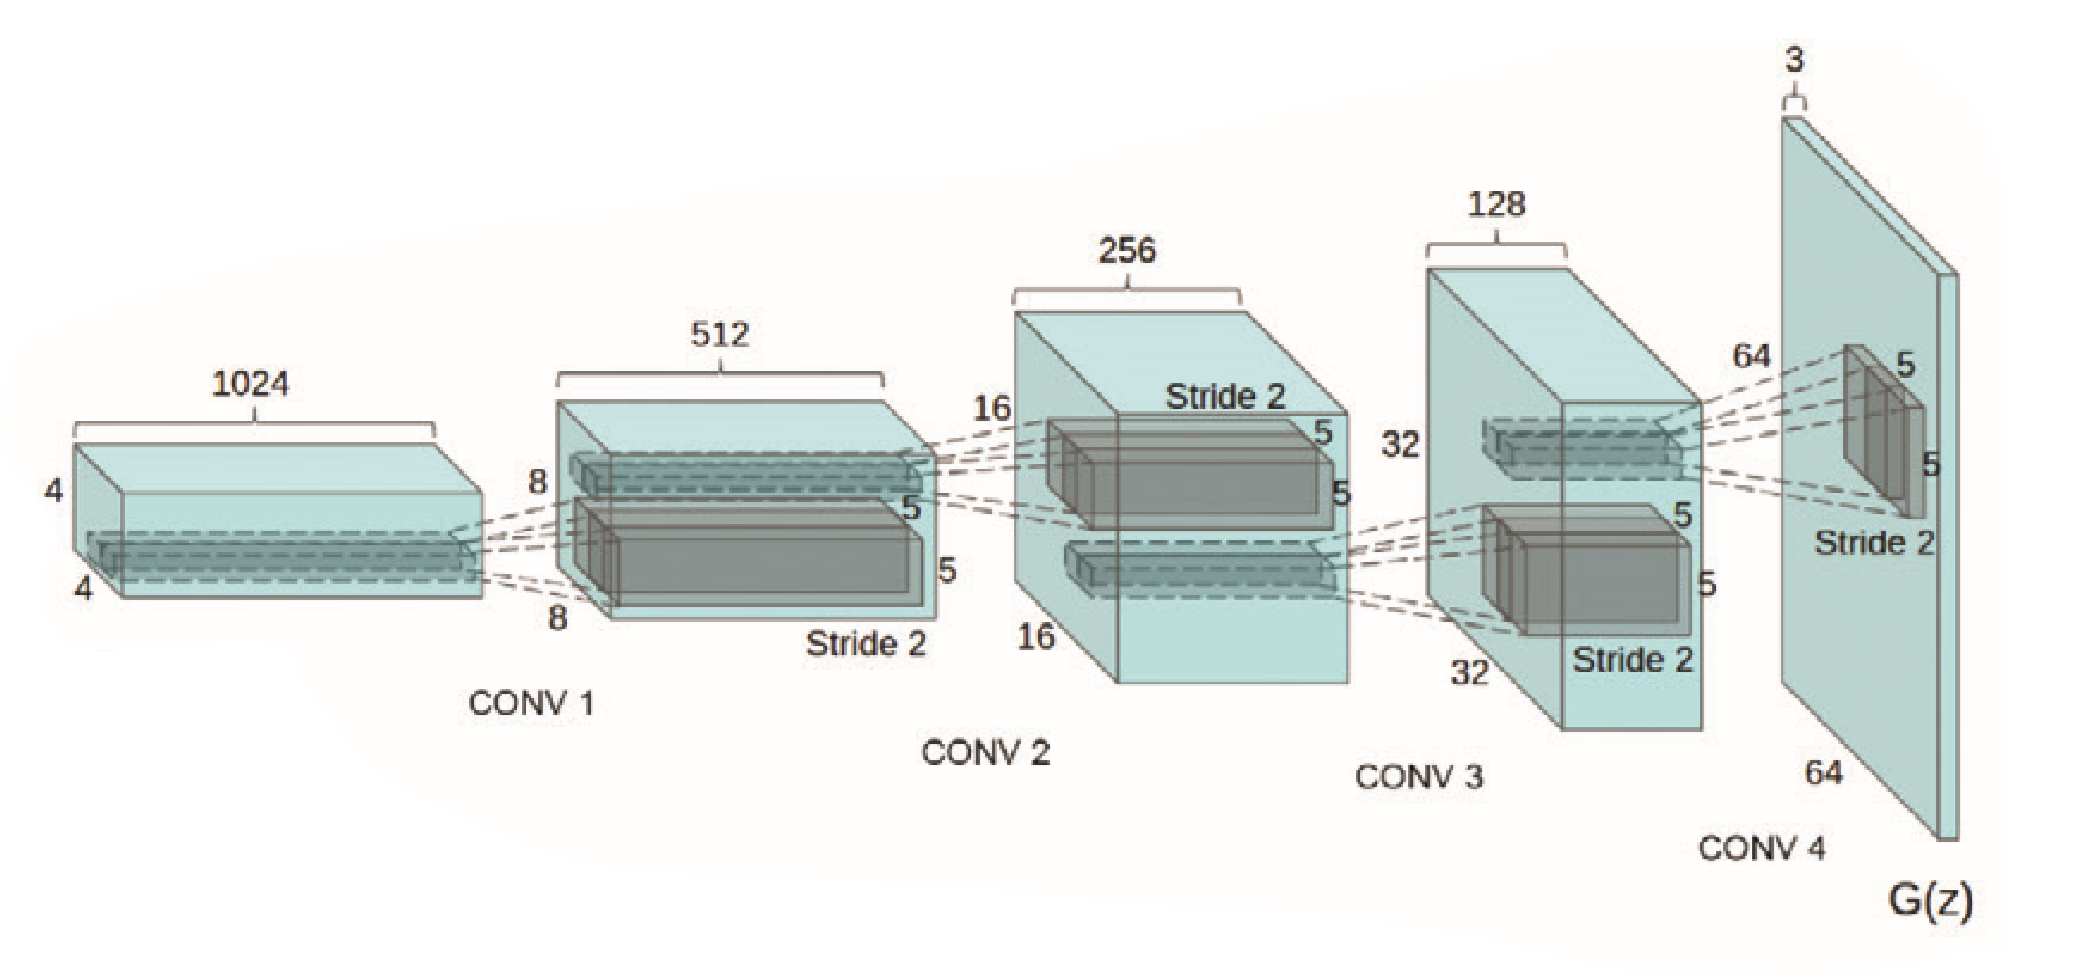
\includegraphics[width=0.85\textwidth]{cnn_3d}
	\vspace*{-3mm}
	\caption[Beispiel eines CNNs mit mehreren Feature Maps]{Ein Beispiel eines CNNs mit steigenden Feature Maps pro Layer \cite[S.138]{DEEP_LEARNING_REVOLUTION}.}
	\label{fig:cnn_3d}
\end{figure}
\vspace*{-5mm}
Die Anzahl der Feature Maps steigt in der Regel mit der Tiefe an, jedoch sollte sich ihre Größe verringern. Dies geschieht entweder über eine Schrittweite oder weiterer Methoden wie den Pooling Layern.
\subsubsection{Pooling Layer}
Pooling Layer werden genutzt um die Größe von Convolutional Layern zu verringern, indem sie zwischen diesem platziert werden und jede Feature Map oder jeden Kanal auf eine gewisse Weise verarbeiten. Die Art der Verarbeitung ist dabei abhängig vom Typ des Pooling Layers, jedoch sind Average oder Max Pooling die typischen Varianten. Beim Max Pooling wird aus einem Filter einer gewissen Höhe und Breite der Größte Wert in diesem Bereich der Feature Map entnommen. Dadurch kann dessen Größe stark verringert werden. Auch können Pooling Layer wieder eine gewisse Schrittweite (Stride) haben, mit denen die Verringerung der Größe einer Feature Map erhöht werden kann \cite[S.18-19]{DEEP_LEARNING_CV}\cite[S.369-370]{MACHINE_LEARNING}. In der Folgenden Abbildung wird die Arbeitsweise eines 2 x 2 Max Pooling mit einem Stride von 2 dargestellt: 
\begin{figure}[H]
	\centering
	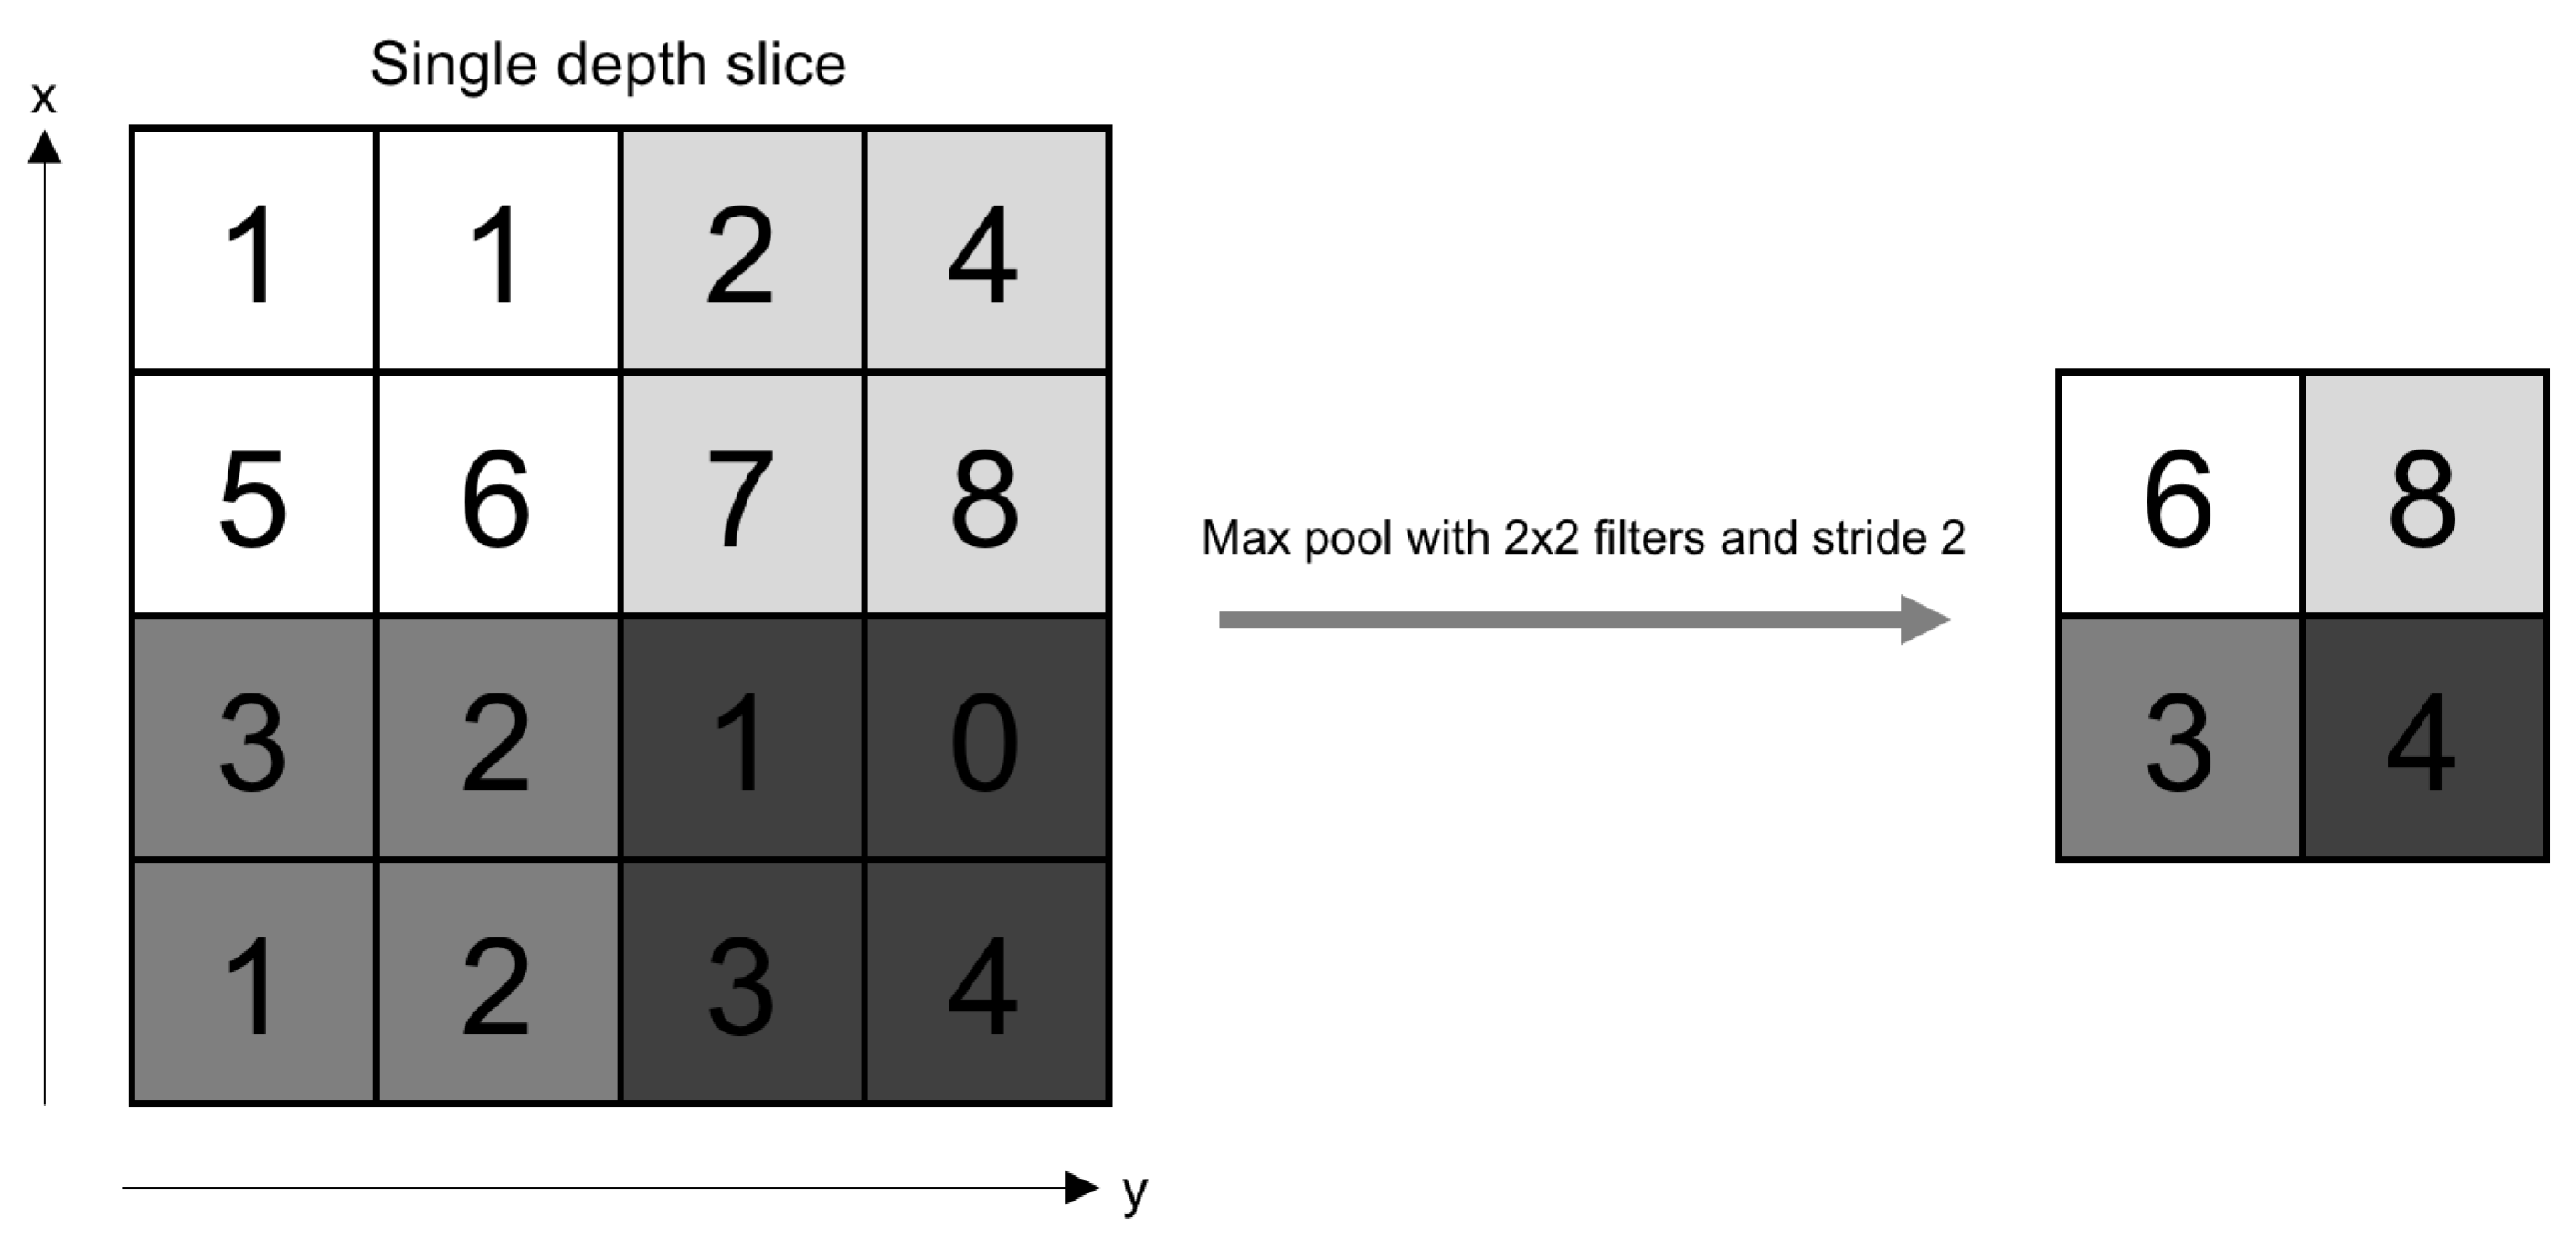
\includegraphics[width=0.85\textwidth]{pooling}
	\vspace*{-3mm}
	\caption[Arbeitsweise des Max Pooling]{Die Arbeitsweise des Max Pooling mit einem 2 x 2 Kernel und Stride von 2 \cite[S.19]{DEEP_LEARNING_CV}.}
	\label{fig:pooling}
\end{figure}
\vspace*{-5mm}
Mit der Definition der Pooling Layer sind nun die wichtigsten Grundlagen für das Maschinelle Lernen mit Bildern gesetzt. Es kann also nun mit dem praktischeren Aspekten begonnen werden.
\section{Datensätze}
Die verwendeten Datensätze stammen von der Online-Community Kaggle. Kaggle veranstaltet Data-Science Wettbewerbe und erlaubt es Datensätze zu finden und bereitzustellen. Die Erkennung von Fingeralphabeten ist ein übliches Problem der Bilderkennung, sodass diverse Datensätze zur Auswahl stehen. Im Projekt wurden zwei Datensätze genutzt die nachfolgend näher beschrieben werden.
\subsection{Sign Language MNIST Dataset}
Der „Sign Language MNIST“ Datensatz wurde unter Eingrenzung in Bezug auf Support Vektor Maschinen bereits kurz angesprochen. Der Datensatz war bereits aufbereitet und die Merkmale der Bilder wurden in Form von Graustufen (0-255) in eine CSV Datei geschrieben. Die CSV-Datei enthielt mit einer Klasse und 28x28 Pixeln pro Datensatz 785 Spalten. Die Buchstaben Z und J wurden nicht als Klassen hinterlegt, da diese eine gewisse Gestik benötigen die in einem Standbild nicht einzufangen ist. Durch extrahieren der Merkmale konnten die Bilder zurückgewonnen und manuell analysiert werden. Aufgefallen ist, dass die Bilder stets mit einem ruhigen und einfarbigen Hintergrund aufgenommen wurden. Insgesamt lagen in einem 80 zu 20 Verhältnis 27455 Trainingsdaten und 7172 Testdaten vor. Die geringe Anzahl an Merkmalen erlaubte ein schnelles Training, allerdings mussten für eine reale Anwendung die Bilder runterskaliert und aufbereitet werden. Trotz hoher Accuracy auf dem Testdatensatz, konnten Bilder in einer Real-Welt-Anwendung mit einer Webcam nicht zuverlässig erkannt werden. Begünstigt wurde dieses Problem vermutlich durch die geringe Informationsdichte der Bilder. Daraufhin wurde der Datensatz gewechselt. 
%TODO: QUELLE EINFÜGEN
\subsection{ASL Alphabet Dataset}
Der zweite Datensatz mit den Namen „ASL Alphabet“ hat 87000 Bilder mit Farbinformationen und 200x200 Pixeln und ist damit deutlich größer als der vorherige. Die Input-Größe, berechenbar durch Breite x Höhe x Farbinformation, ist für ein Konvolutionelles Neuronales Netz dank dem später erklärten Filtern und dem möglichen Trainieren auf einem Grafikprozessor kein Problem. Das ConvNet ist in der Lage die wichtigen Informationen selbst zu extrahieren und die unwichtigen herauszufiltern. In dem Datensatz sind zusätzlich die Klassen Space, Delete und Nothing enthalten, wobei nur letztere berücksichtigt wurde. Die Handzeichen sind durchweg vor dem gleichen Hintergrund aufgenommen, variieren aber etwas stärker in Lichtverhältnissen, Bildschärfe und Position der Hand. Außerdem ist der Hintergrund nicht einfarbig, sondern die Bilder scheinen vor einem Dachfenster aufgenommen worden zu sein. Anders als der Sign Language MNIST Datensatz sind die Bildinformationen nicht bereits in eine CSV Datei extrahiert, sondern liegen tatsächlich als Bilder vor. Die einzelnen Handzeichen sind in Ordnern mit dem Namen des jeweiligen Buchstaben organisiert. Ein Testdatensatz ist bereits vorbereitet, enthält aber lediglich ein Bild jeder Klasse, sodass dieser noch erweitert wird. Das genaue vorgehen wird unter \ref{aslpreparation} beschrieben.
%TODO: QUELLE EINFÜGEN
\subsection{Videodatensätze}
%TODO: TEXT EINFÜGEN
\section{Entwicklungsprozess}
Da nun die genutzten Datensätze beschrieben wurden, kann mit der Dokumentation des Entwicklungsprozesses fortgefahren werden. Hier wird wie bei Maschinellen Lernen üblich sich zunächst auf die Datenvorverarbeitung konzentriert.
\subsection{Datenvorverarbeitung}
Da die beiden hauptsächlich verwendeten Datensätze in einer für ihre Auflösung ausreichende Qualität vorhanden sind, müssen nur noch wenige Schritte in der Datenvorverarbeitung beachtet werden. Dies bezieht sich vor allem auf das Einlesen der Datensätze und das Skalieren der Bilder. Hier liefern Keras und Tensorflow in den neuesten tf-nightly Versionen (getestet mit 2.3.0a20200613) mit \lstinline[language=pythoninline]|image_dataset_from_directory| eine sehr mächtige Funktion, welche lediglich auf Basis von Ordnerstrukturen Bildatensätze mit passenden Labels erstellt und auch das Skalieren von Bildern übernehmen kann \cite{KERAS_IMAGE_PREPROCESSING}. Dabei wird beim Aufruf ein Tensorflow Dataset zurückgegeben, das bereits Pipelining einer gewissen Batchgröße von der Festplatte unterstützt. Dies ist bei sehr großen Datensätzen nützlich. Nun, müssen die Datensätze lediglich in passenden Ordnerstrukturen umgewandelt werden, bei denen alle Bilder einer Klasse einen Ordner mit passender Bezeichnung nutzen. Außerdem ist eine Teilung in Test, sowie Trainings- und Validierungsdaten nötig, denn \lstinline[language=pythoninline]|image_dataset_from_directory| unterstützt lediglich eine Zweiteilung. 
\subsubsection{Sign Language MNIST Dataset}
Dieser Datensatz besteht im Kern aus zwei CSV Dateien für Training- und Test. Die Zeilen repräsentieren dabei die 28x28 Pixel eines Grauwertbildes, sowie ein Label in der ersten Spalte. Die Label sind Zahlen von 0-25 und repräsentieren alle Buchstaben des Alphabets außer Z (25) und J (9), welche ausgelassen wurden. Trotz des Aufbaus in CSV Dateien, wurde sich entschieden die Werte zu extrahieren und als einzelne PNGs in die erforderlichen Ordnerstrukturen abzuspeichern. Der Kern der Skriptdatei zur Vorverarbeitung des Sign Language MNIST Dataset ist dabei folgende Funktion:
\begin{lstlisting}[language=python,firstnumber=36,caption={Kern der Sign Language MNIST Dataset Vorverarbeitung.},label=lst:to_image_at_dir]
def to_image_at_dir(target_dir, row_data, image_name):
	"""
	Wandelt die Zeilen einer CSV Datei im Datensatz in ein Bild um.
	:param target_dir: Zielordner
	:param row_data: Daten der Zeile.
	:param image_name: Name des Bildes.
	:return: None.
	"""
	# Label entnehmen.
	label = row_data[0]
	# Daten entnehmen in Integer umwandeln.
	list_data = list(map(int, row_data[1::]))
	
	# Image Data in Numpy 28x28 Array umwandeln.
	image_data = numpy.reshape(numpy.array(
	list_data, dtype=numpy.uint8), (28, 28))
	label_folder = target_dir + str(label) + "/"
	
	# Ordner erstellen, wenn nicht vorhanden.
	os.makedirs(label_folder, exist_ok=True)
	# Bild erstellen.
	image = Image.fromarray(image_data)
	# Bild als PNG speichern.
	image.convert("RGB").save(label_folder + image_name + ".png")
\end{lstlisting}
Diese Funktion ist sehr einfach und nimmt lediglich einen Zielordner, die Daten einer Zeile des Datensatzes sowie ein Name des Bildes (zum Beispiel eine Bildnummer) an. Dann werden in Zeile 45 und 47 Label und Daten getrennt. Eine Umwandlung in Integer der Daten wird ebenfalls über eine Map-Funtkion vorgenommen. Es folgt in Zeile 50 bis 52 eine Umwandlung in ein 28x28 Numpy-Array mit Datenpunkten als 8-Bit Unsigned Integer (uint8). Zuletzt werden die Daten des Numpy-Arrays lediglich mit der bekannten Bildverarbeitungsbibliothek für Python Pillow in ein Bild umgewandelt und anschließend als PNG in RGB abgespeichert. Es wurde sich hier für PNGs statt für Grauwertbilder entschieden, da so ein problemloses Verwenden von \lstinline[language=pythoninline]|image_dataset_from_directory| möglich wird.
\subsubsection{ASL Alphabet Dataset}
\label{aslpreparation}
Der ASL Alphabet Dataset ist vom Aufbau deutlich einfacher zu verarbeiten, da hier die Bilder bereits in passende Subordner des Trainingsdatensatzes sortiert sind. Die Testdaten benötigen allerdings Vorverarbeitung, da diese pro Zeichen der ASL nur ein Bild beinhalten. Dies ist nicht hinreichend für Testdaten. In der Vorverarbeitung wird also eine bestimmte Anzahl zufälliger Bilder pro ASL Zeichen aus den Trainingsdaten ausgewählt und in das passend erstellte Verzeichnis für die Testdaten umkopiert.
\\\\
Dies funktioniert im Kern über folgende Funktion, welche jeden Ordner für ein ASL Zeichen durchläuft und mittels der Bibliothek \lstinline[language=pythoninline]|glob| alle Dateien aus diesen ließt. Dann werden mit \lstinline[language=pythoninline]|random.sample| eine vorher definierte zufällige Anzahl von Samples (in der Praxis 300) ausgewählt und in das Zielverzeichnis des Testordners für dieses ASL Zeichen umkopiert.
\begin{lstlisting}[language=python,firstnumber=44,caption={Kern der Sign Language MNIST Dataset Vorverarbeitung.},label=lst:to_image_at_dir]
# Bewege die in rand_num_to_move definierte Anzahl 
# zufälliger Elemente pro Klasse in den Testordner.
for target_dir_name in glob.glob(target_directory + "/" + 
		train_directory_name + "/*"):
	
	target_dir_classes = glob.glob(target_dir_name + "/*")
	# Wähle für diese Klasse rand_num_to_move zufällige Elemente aus.
	random_elements = random.sample(target_dir_classes, 
		rand_num_to_move)
	# Kopiere die Elemente um.
	for move_element in random_elements:
		new_dir = move_element.replace(train_directory_name, 
			test_directory_name)
		os.makedirs(os.path.dirname(new_dir), exist_ok=True)
		shutil.move(move_element, new_dir)
\end{lstlisting}
\subsubsection{DatasetParser Pakete}
Das Ziel der DatasetParser Python Pakete ist es, für alle vorverarbeiteten Datensätze eine vereinigte Schnittstelle zum Bereitstellen von Datensätzen zu liefern. Diese bestehen aus einer DatasetParser Datei mit den Funktionen \lstinline[language=pythoninline]|get_train_and_val| und \lstinline[language=pythoninline]|get_test|, welche Trainings-, Test- und Validierungsdaten bereitstellen, sowie den Konstanten \lstinline[language=pythoninline]|class_names| und \lstinline[language=pythoninline]|image_size|, die Klassennamen (im Bezug auf die Ordner der vorverarbeiteten Datensätze) und eine standardmäßige Bildgröße definieren. Eine weitere in den Paketen nötige Skriptdatei ist DatasetPrepareOrig. Diese führt mittels einer separaten Ausführung eine in den vorherigen Kapiteln beschriebene Vorverarbeitung aus. Der Datensatz selber ist nun in DatasetOrig, als nicht verarbeiteter Datensatz, und in DatasetPrepared, als durch das Skript vorverarbeiteter Datensatz, definiert.
\\\\
Die Arbeitsweise der DatasetParser Dateien ist nun sehr einfach zu beschreiben. Diese führen beim Aufruf von \lstinline[language=pythoninline]|get_train_and_val| zweimal die Tensorflow-Funktion \lstinline[language=pythoninline]|image_dataset_from_directory| mit vom Datensatz abhängigen Parametern auf und geben die Ergebnisse dieser zurück. Wird unter der Angabe des Parameters \lstinline[language=pythoninline]|validation_split| diese Funktion auf ein Verzeichnis zweimal ausgeführt, so gibt Tensorflow beim ersten Aufruf das Dataset der Trainings- und beim zweiten das Dataset der Validierungsdaten zurück. Die Testdaten der Funktion \lstinline[language=pythoninline]|get_test| werden über einen einzelnen Aufruf ohne \lstinline[language=pythoninline]|validation_split| zurückgegeben.
\begin{lstlisting}[language=python,firstnumber=1,caption={Beispielhafter Aufruf der Funktion zum Einlesen von Daten},label=lst:dataset]
return image_dataset_from_directory(
	directory="datasets/kaggle_1/DatasetPrepared/train",
	label_mode='categorical',
	color_mode='grayscale',
	image_size=image_size_param,
	batch_size=batch_size,
	shuffle=shuffle,
	seed=seed,
	validation_split=validation_split,
	subset="training",
	interpolation='bilinear',
	follow_links=False
)
\end{lstlisting}
Im Listing \ref{lst:dataset} wird ein Aufruf der Funktion \lstinline[language=pythoninline]|image_dataset_from_directory| beschrieben. Die wichtigsten Parameter haben dabei folgende Aufgaben:
\begin{itemize}
	\item \lstinline[language=pythoninline]|directory|: Das Verzeichnis aus dem der Datensatz gelesen wird.
	\item \lstinline[language=pythoninline]|label_mode|: Bei categorical werden die Subordner als Kategorien gesehen und als One-Hot kodierten Vektor beschrieben.
	\item \lstinline[language=pythoninline]|color_mode|: Umgewandelte Farbkanäle der Bilder.
	\item \lstinline[language=pythoninline]|image_size|: Skalierte Größe der Bilder.
	\item \lstinline[language=pythoninline]|batch_size|: Größe der Batches des Datasets.
	\item \lstinline[language=pythoninline]|shuffle|: Werden die Bilder nach dem Einlesen zufällig angeordnet.
	\item \lstinline[language=pythoninline]|validation_split|: Anteil der Validierungsdaten.
	\item \lstinline[language=pythoninline]|subset|: Das zurückgegebene Subset für dieses Verzeichnis. Dieses ist entweder training oder validation.
	\item \lstinline[language=pythoninline]|interpolation|: Genutztes Verfahren für die Skalierung.
\end{itemize}
Da die Datensätze für ihre Auflösung alle eine sehr rauschfreies Bild aufweisen und in der Regel schon recht gut auf die Hände fokussiert sind, ist damit nun die Datenvorverarbeitung abgeschlossen und die Bilder der Datensätze können sehr einfach in passende Tensorflow-Datasets gelesen werden. Nun, wird die Entwicklung und Auswertung von Modellen beschrieben.
\subsection{Entwickelte Modelle}
In diesem Kapitel wir der Grundaufbau der Python-Dateien zum Maschinellen Lernen vorgestellt und die Ergebnisse einiger Modelle vorgestellt. Dabei werden für Neuronale Netze, Konvolutionelle Neuronale Netze und Transferlearning einige der besten Versuche vorgestellt. 
\subsubsection{Grundaufbau des Modelltrainings}
Alle Dateien für das Training von Modellen haben grundsätzlich einen ähnlichen Aufbau. Zunächst müssen die DatasetParser der gewünschten Datensätze inkludiert werden mit welchen ein Großteil der Datenvorverarbeitung schon erledigt werden kann. Danach folgen in der Regel einige Definitionen für Batchgröße und Bildgröße, mit welchen nun die Funktionen \lstinline[language=pythoninline]|get_train_and_val| und \lstinline[language=pythoninline]|get_test| aufgerufen werden können. Dank sinnvoller Default-Parameter ist dieser Aufruf in der Regel recht kurz. Es wurde ein 80-20 Validation Split unter einer in Kapitel \ref{validation} beschriebenen Validierung in drei Stufen verwendet. Am Ende der Vorbereitung wird in der Regel noch die Anzahl der Klassen für die Ausgabe und die Größe der Eingabe für den ersten Layer des Modells definiert. Ein Beispiel für die Vorbereitung des Trainings ist im folgenden Listing zu erkennen:
\begin{lstlisting}[language=python,firstnumber=1,caption={Beispielhafte Vorbereitung für das Training},label=lst:pre_train]
from sign_language_image.datasets.kaggle_1.DatasetParser
	import get_train_and_val, get_test, class_names 
...
# Batchgröße
batch_size = 100
# Bildgröße
image_size = (28, 28)
train_ds, val_ds = get_train_and_val(batch_size, 
	image_size_param=image_size)
test_ds = get_test(image_size_param=image_size)

# Anzahl der Klassen aus den Namen der Klassen extrahieren
num_of_classes = len(class_names)
# Input Shape als Bildgröße + Farbkanäle
input_shape = (image_size[0], image_size[1], 1)
\end{lstlisting}
Danach kann dann schon ein Modell definiert werden. Diese können sich je nach Aufbau etwas unterscheiden, daher wird auf sie und ihre Ergebnisse in den nächsten Kapiteln eingegangen.
\\\\
Nach der Definition eines Modells kann dieses kompiliert und mit einem Optimizer und Qualitätsmaß versehen werden. Hier wurde aufgrund des Aufbaus der Daten und des Lernziels die Kreuzentropie genutzt. Außerdem wird ein Modell während der Optimierung über die Vorhersagegenauigkeit auf Trainings- und Validierungsdaten ausgewertet. Dies ist aufgrund der gleichmäßigen Verteilung und Priorität der Klassen in den Datensätzen möglich. Als Optimierer wird eine Erweiterung des stochastische Gradientenverfahren den Adam-Optimierer genutzt.
\begin{lstlisting}[language=python,firstnumber=1,caption={Kompilierung eines Modells},label=lst:compile_model]
# Modell kompilieren mit Kreuzentropie und Adam Optimizer.
model.compile(loss='categorical_crossentropy',
	optimizer=tf.keras.optimizers.Adam(lr=0.00005),
	metrics=['accuracy'])
\end{lstlisting}
Dann wurde eine Funktion für das Loggen entwickelt. Diese kopiert das momentan aktive Skript in einen eigenen Ordner eines übergebenen Logverzeichnisses. Dieses dient als Referenz, wenn die originale Trainingsdatei verändert wurde. Dann wird abhängig von einem Parameter die Ausgabe der Konsole in eine Logdatei in dem vorher erstellten Verzeichnis umgeleitet, um später den Trainingsvorgang nachvollziehen zu können. Zuletzt werden zwei Tensorflow-Callbacks für das Verzeichnis erstellt, welche TensorBoard-Logs erstellen und die Modelle mit dem geringsten Fehler abspeichern.
\begin{lstlisting}[language=python,firstnumber=1,caption={Logging Funktion für Trainingsvorgänge},label=lst:log_train]
def log_run(log_dir, log_to_file=True):
	script_path = sys.argv[0]
	script_name = os.path.basename(script_path)
	log_dir_script = log_dir + script_name + "_" + 	 datetime.now().strftime("%d-%m-%Y_%H%M%S") + "/"
	# Erstelle das Log Verzeichnis
	os.makedirs(log_dir_script)
	# Kopiere das Script, welches ausgeführt wurde in das Log Verzeichnis
	shutil.copy(script_path, log_dir_script + script_name)
	# Leite Ausgabe der Konsole um
	if log_to_file:
		print("Starting Log To File!")
		sys.stdout = open(log_dir_script + script_name + 
			".log.txt", "w")
	
	# Erstelle und gebe Callbacks für das Log-Verzeichnis zurück.
	return tf.keras.callbacks.TensorBoard(
		log_dir=log_dir_script, profile_batch=5), \
		tf.keras.callbacks.ModelCheckpoint(log_dir_script + 'model.mdl_wts.hdf5', save_best_only=True,
		monitor='val_loss', mode='min'), log_dir_script
\end{lstlisting}
Im Folgenden wird lediglich nur noch ein Callback eingeführt, welches das Training nach einer gewissen Zahl von Durchläufe in welchen sich der Fehler des Modells nicht verbessert abbricht. Dann kann das Modell mit Trainingsdaten und Validierungsdaten zur Überprüfung folgendermaßen für eine maximale Anzahl von Epochen antrainiert werden:
\begin{lstlisting}[language=python,firstnumber=1,caption={Start des Trainings mit Keras},label=lst:train_start]
model.fit(train_ds,
	epochs=50,
	verbose=1,
	validation_data=val_ds,
	callbacks=[tensorboard_callback, checkpoint, es])
\end{lstlisting}
Nach dem Trainingsvorgang wird nun die beste Epoche aus dem Logverzeichnis geladen und mit den Testdaten überprüft. Dann wird zunächst die \lstinline[language=pythoninline]|evaluate| Methode des Keras-Modells genutzt, um eine Vorhersagegenauigkeit und den Fehler auf den Testdaten zu bestimmen. Zum Schluss wird mittels Scikit-Learn in der eigens definierte \lstinline[language=pythoninline]|evaluate| Funktion eine Konfusionsmatrize und Auswertungstabelle mit Precision, Recall und F1-Score zu den Testdaten erstellt. Dies ist im folgenden Listing erkennbar:
\begin{lstlisting}[language=python,firstnumber=1,caption={Auswertung eines Modells mit Testdaten},label=lst:modell_eval]
# Lade das beste Modell
model = load_model(run_path + "model.mdl_wts.hdf5")
# Score auf den Testdaten
score = model.evaluate(test_ds, verbose=1)
print('Test loss:', score[0])
print('Test accuracy:', score[1])

# Entnehme aus dem Test Datensatz, zur Anwendung mit sklearn
test_data_labels = []
for data, label in test_ds.take(-1):
	test_data_labels.extend(label)

# Prediction für den Test Datensatz
pred = model.predict(test_ds, verbose=1)
# Evaluiere die Ergebnisse vom Testdatensatz mit sklearn
evaluate(numpy.argmax(pred, axis=1), 
	numpy.argmax(test_data_labels, axis=1))
\end{lstlisting}
Abschließend sei erwähnt, dass die Auswertungsergebnisse der Testdaten nur in Betracht gezogen wurden, wenn bereits einige andere Modelle mit Validierungsdaten getestet wurden. Ein anderes Auswertungsverhalten würde die in Kapitel \ref{validation} genannten Grundsätze verletzen.
\subsubsection{Neuronale Netze}
\label{nntraining}
Zunächst wurde der Einsatz einfacher Neuronaler Netze erprobt. Da diese grade bei großen Bildern in der Regel von CNNs abgelöst wurden, wurden hier nur wenige Tests ausgeführt. Selbst bei großen Modellen und ohne vorliegenden Overfitting Effekten, konnte maximal eine Vorhersagegenauigkeit von 80\% erreicht werden. Grundsätzlich wurde versucht in der Eingabeschicht in etwa ein Neuron pro Bildpunkt zu nutzen. Diese sollten dann in jedem Layer mit einer abnehmenden Schichtgröße immer weiter heruntergerechnet werden, bis es sinnvoll wurde die Ausgabeschicht anzusetzen. Weiterhin wurden alle versteckten Schichten von einem Dropout und einer Batch Normalisierung gefolgt. Auf dieser Basis wurden viele Netzstrukturen erprobt. Eines dieser Modelle, welches für das Sign Language MNIST Dataset verwendet wurde, ist in folgender Abbildung zu erkennen: 
\begin{figure}[H]
	\centering
	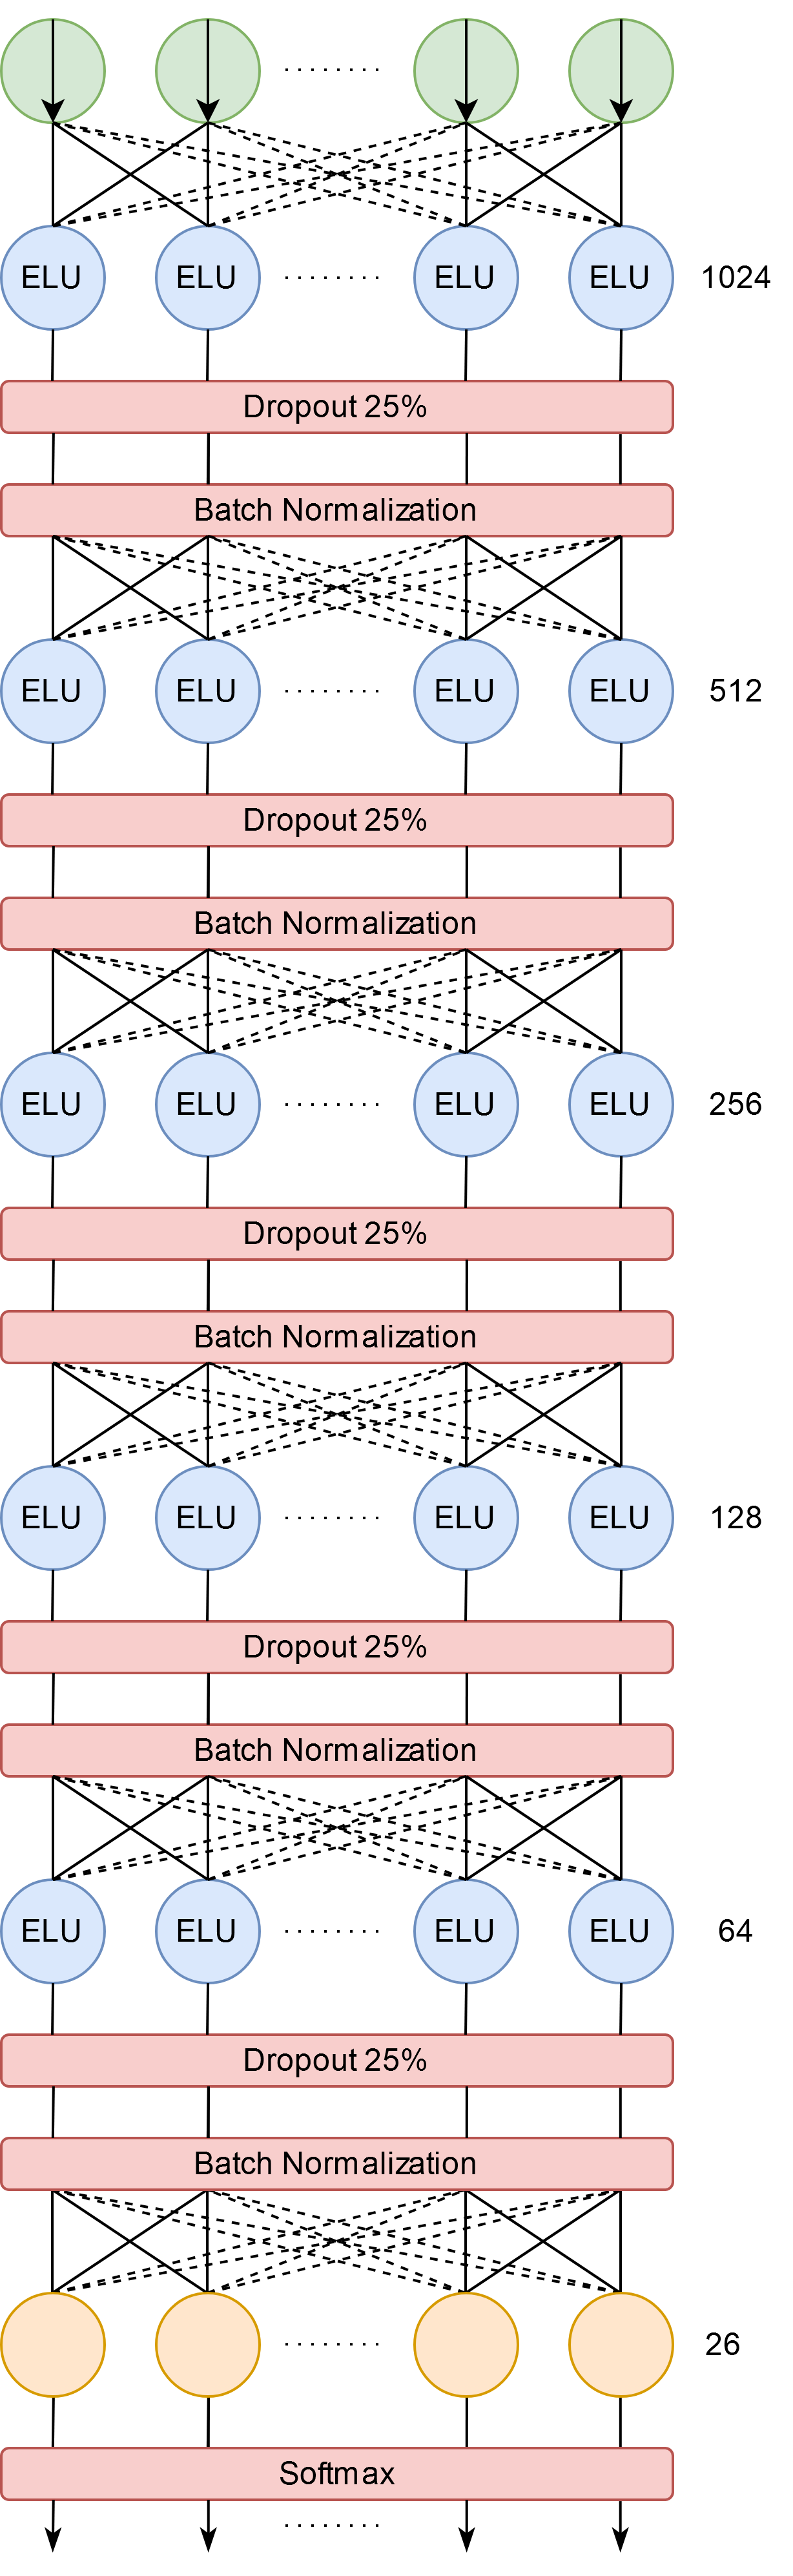
\includegraphics[width=0.50\textwidth]{nn_1}
	\vspace*{-3mm}
	\caption[Eingesetztes Neuronales Netz mit fünf Hidden-Layern]{Ein eingesetztes Neuronales Netz mit fünf Hidden-Layern.}
	\label{fig:nn_1}
\end{figure}
\vspace*{-5mm}
Dieser erreicht auf dem genutzten Datensatz lediglich eine Vorhersagegenauigkeit von 78\% auf den Validierungsdaten. Auf den Testdaten erreicht dieses Modell 81\% Vorhersagegenauigkeit. Dies ist zwar etwas besser, jedoch nicht in einem gewünschten Bereich.
\\\\
Mit dem ASL-Alphabet Dataset gibt es noch größere Probleme im Einsatz normaler Neuronaler Netze. Die Bilder weisen alle eine Größe von 200x200 Pixeln auf, was in einer Eingabegröße von 40000 Pixeln mit drei Kanälen resultieren würde. Die eingegebenen Bilder werden beim Einlesen daher auf 50x50 Grauwerte reduziert. Selbst damit wurde ein siebter Layer mit 2048 ELU-Neuronen an den Anfang des Netzes eingeführt, um die 2500 Eingabewerte sinnvoll aufnehmen zu können. Trotz dieser Änderung und dem Test weiterer Netzstrukturen zeigen sich die Probleme für diesen Datensatz klar. Es konnte dabei maximal eine Vorhersagegenauigkeit 67\% erreicht werden. Grade im ASL-Alphabet Dataset wird daher klar, dass für die Lösung dieser Aufgabe Konvolutionelle Neuronale Netze sinnvoller sind.
\subsubsection{Konvolutionelle Neuronale Netze}
Beim Training der Konvolutionellen Neuronale Netze wurden besonders für den ASL-Alphabet Dataset viele Modellstrukturen erprobt. Es wurde sich für eine wie in dem VGG19 vorhandene typische Verdopplung der Feature Maps entschieden \cite{VGG19}, wobei gleichzeitig weniger Convolutional Layer verwendet wurden, um Overfitting zu vermeiden. Gleichzeitig konnten mit dem Einsatz von Stride zum leichten herunterrechnen der Bildinformationen gute Erfahrungen erzielt werden, auch wenn dies im Falle des Sign Language MNIST Datase durch die geringe Bildgröße in der Regel nur in den ersten ein bis zwei Convolutional Layern verwendet werden konnte. Für die vollständig verbundenen Schichten wurde sich für einen ähnlichen Aufbau wie im vorherigen Kapitel entschieden inklusive des Dropouts und der Batch Normalisierung. Mit dem Sign Language MNIST Dataset konnten zwar bessere Ergebnisse erzielt werden als mit einfachen Neuronalen Netzen, jedoch zeigt sich hier klar die geringe Auflösung der Bilder mit 28x28 Pixeln. In allen erprobten Modellstrukturen wurden schlechtere Ergebnisse erzielt als für den ASL-Alphabet Dataset. Ein eingesetztes Modell für diesen mit guten Ergebnissen ist in Folgender Abbildung dargestellt:
\begin{figure}[H]
	\centering
	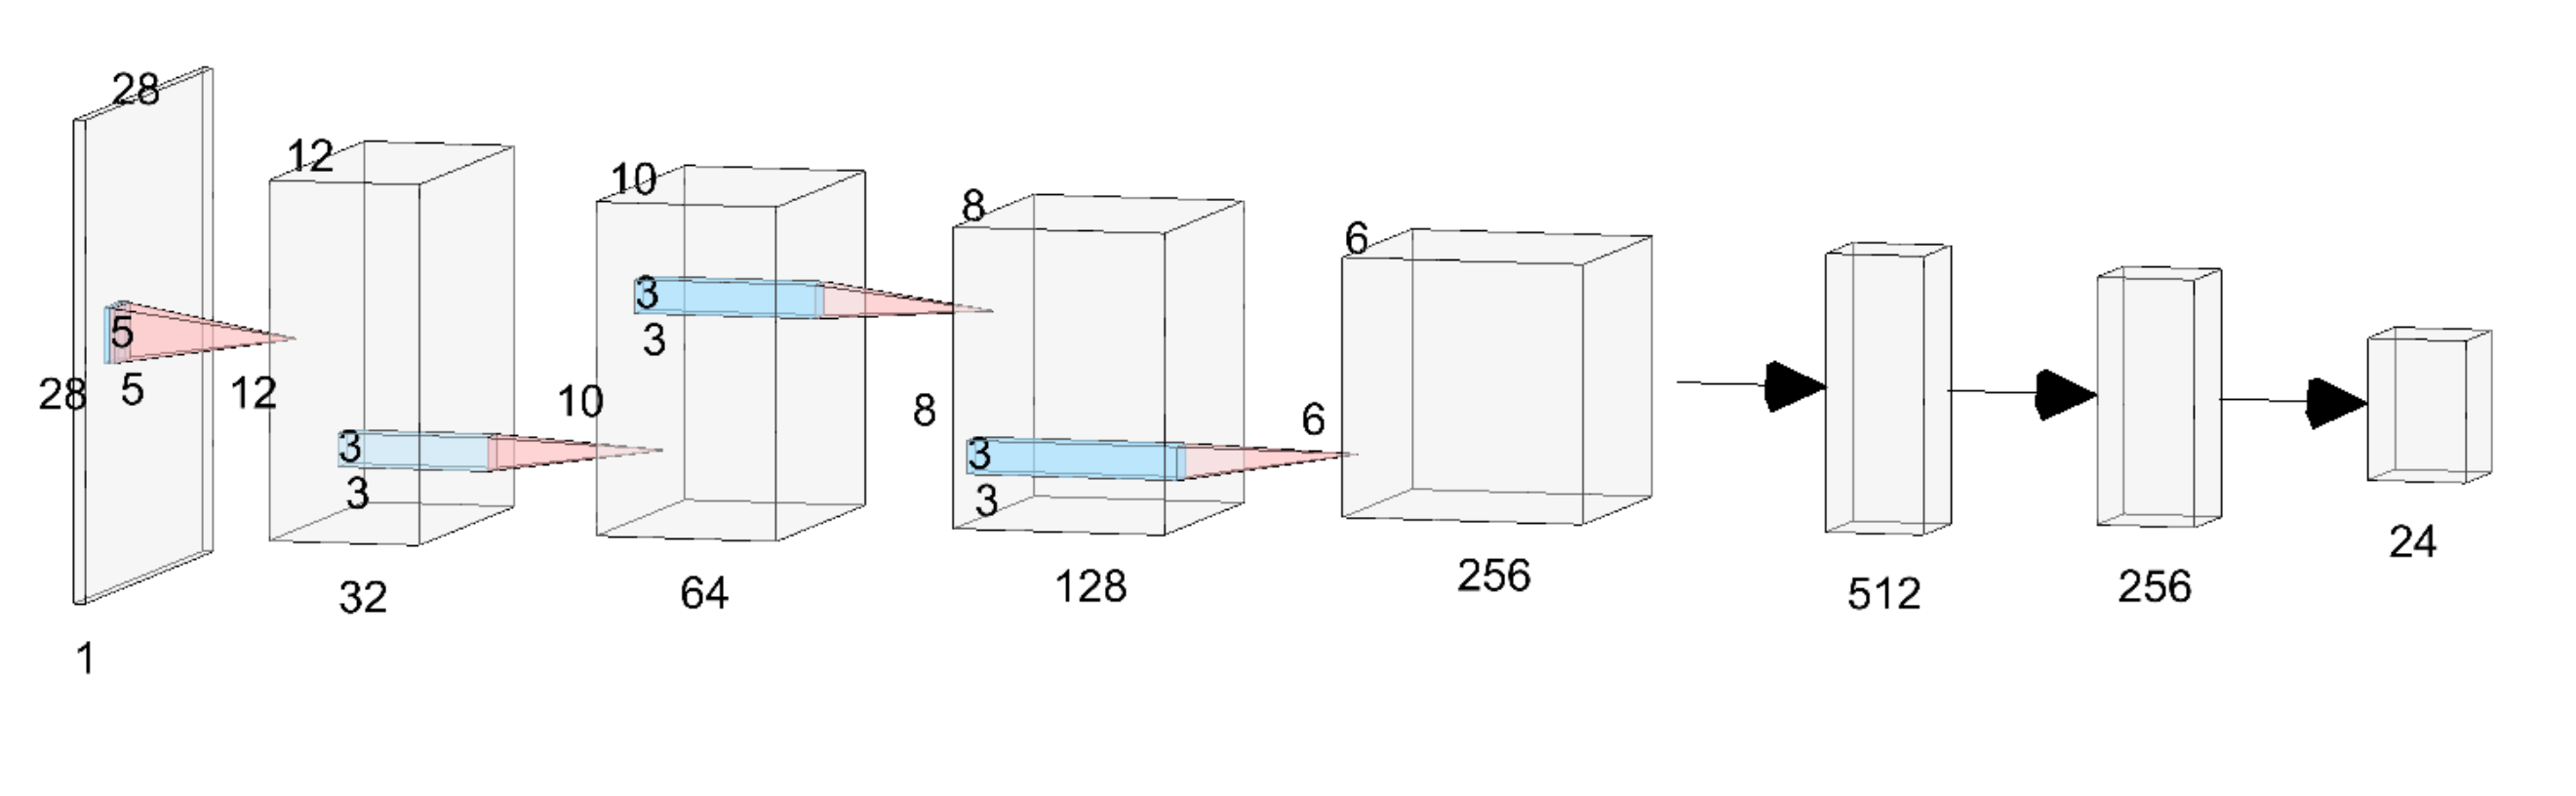
\includegraphics[width=0.90\textwidth]{cnn_example_kaggle_1}
	\vspace*{-3mm}
	\caption[Eingesetztes CNN für den Sign Language MNIST Dataset]{Ein Eingesetztes CNN für den Sign Language MNIST Dataset.}
	\label{fig:cnn_example_kaggle_1}
\end{figure}
\vspace*{-5mm}
Zwar konnten mit diesen Modell eine hundertprozentige Genauigkeit für die Validierungsdaten erreicht werden, es war jedoch nie eine komplette Generalisierung für die Testdaten zu erkennen. Diese erreichen maximale Genauigkeiten von 75\%. Die Gründe für das schlechtere Abschneiden konnten bisher nicht herausgefunden werden. Es wären Fehler in der Vorverarbeitung, dem Einlesen, eine starke Abweichung der Testdaten von den Trainings- und Validierungsdaten oder Overfitting denkbar. Leider konnten dies nicht perfekt gelöst werden und aufgrund besserer Ergebnisse für den ASL-Alphabet Dataset, wurde sich nun auf diesen konzentriert. 
\begin{figure}[H]
	\centering
	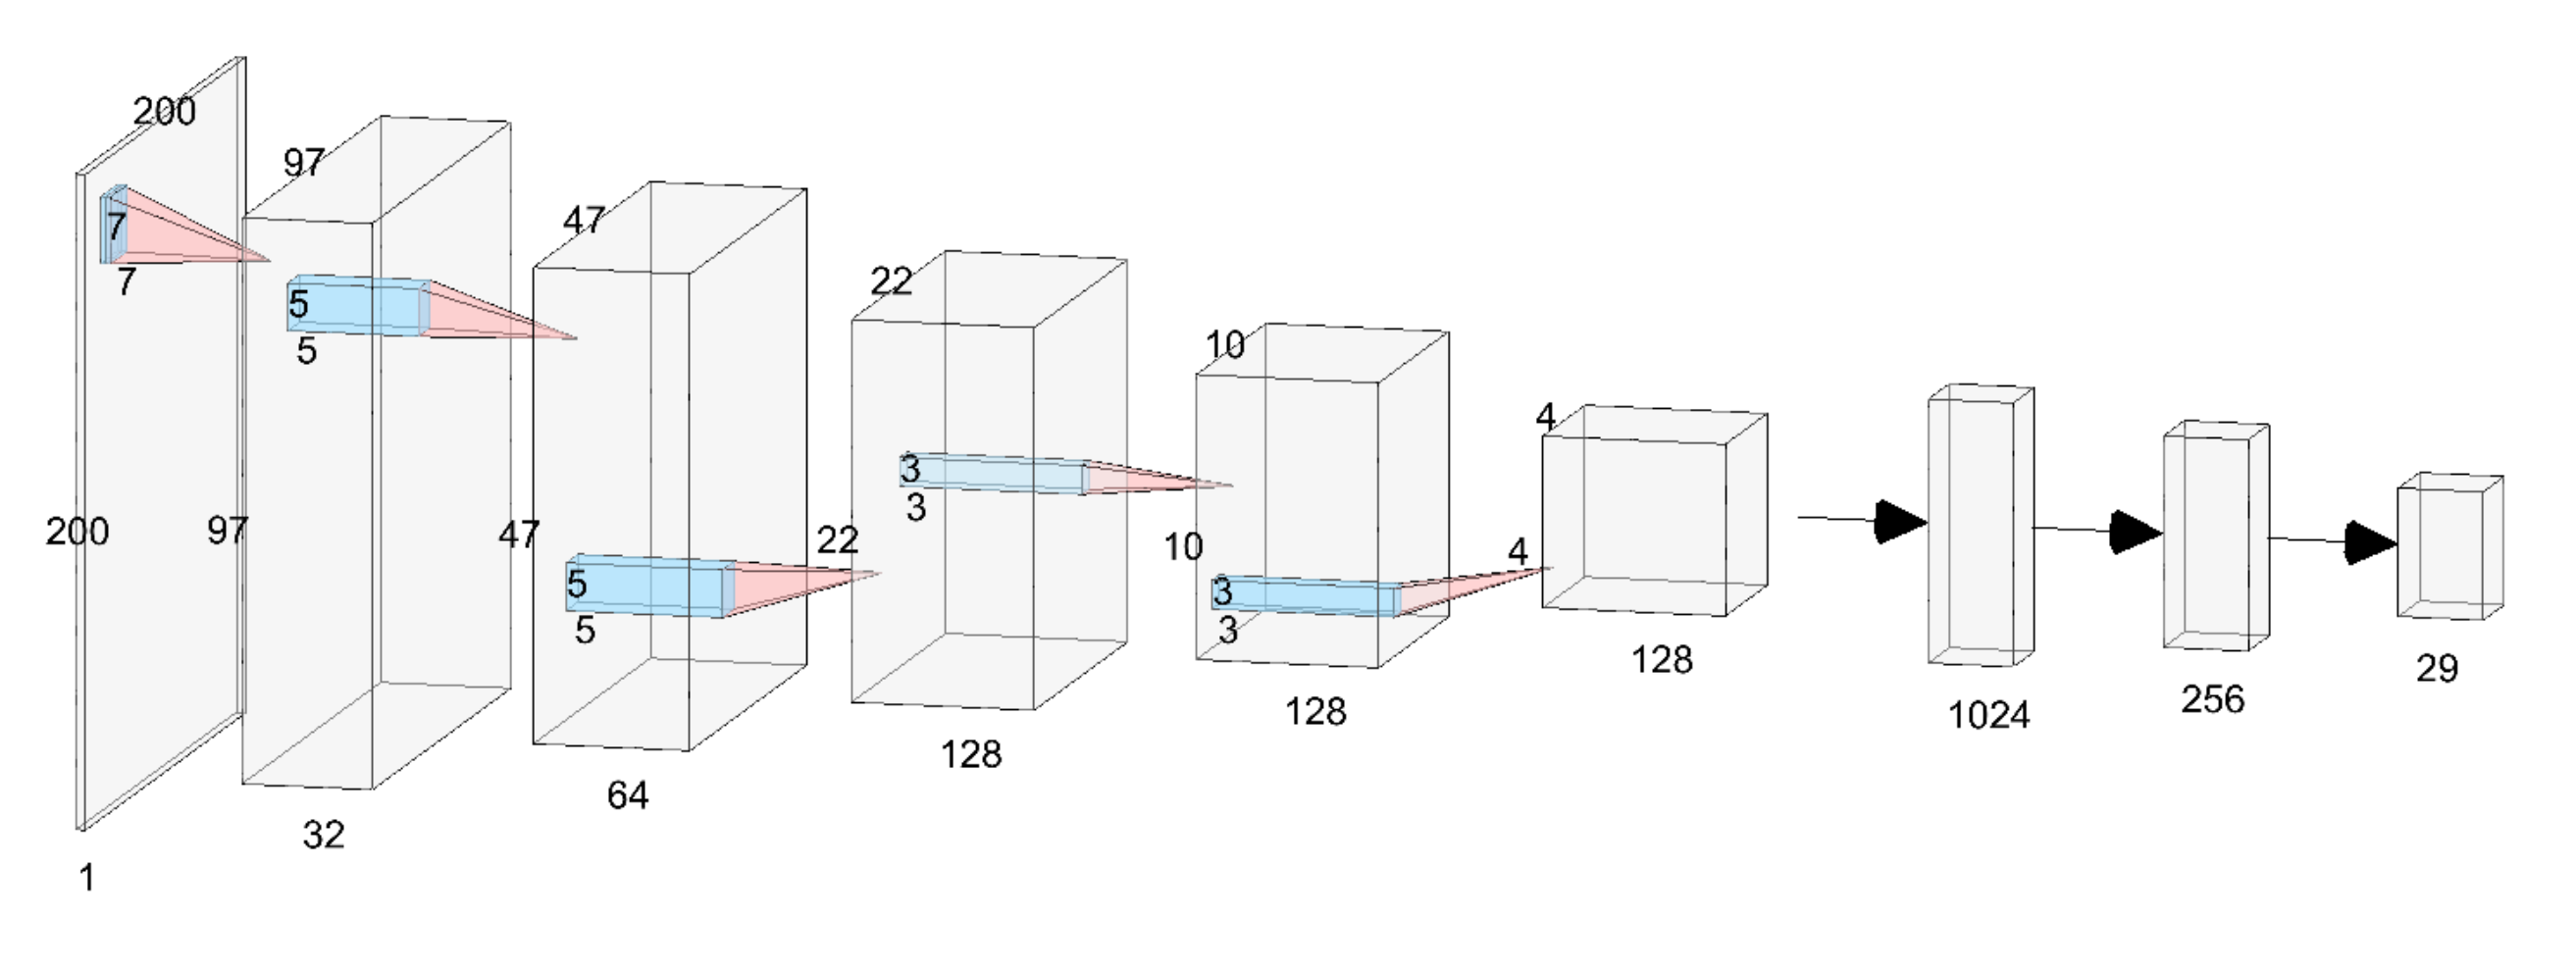
\includegraphics[width=0.90\textwidth]{cnn_used_kaggle_2}
	\vspace*{-3mm}
	\caption[Eingesetztes CNN für den ASL-Alphabet Dataset]{Ein Eingesetztes CNN für den ASL-Alphabet Dataset.}
	\label{fig:cnn_used_kaggle_2}
\end{figure}
\vspace*{-5mm}
Eines dieser Modelle ist in der oberen Abbildung zu erkennen. Dieses konnte sehr gute Ergebnisse erzielen. Es ist erneut leicht an das VGG19 mit weniger Convolutional Layern angelehnt. Aufgrund der höheren Bildgrößen im ASL-Alphabet Dataset weißt es deutlich höhere Parameterzahlen auf als das vorherige Modell. Insgesamt konnte es eine Vorhersagegenauigkeit von 99\% Test- und Validierungsdaten erreichen. Es ist damit bisher und insgesamt eines der besten Modelle für die Vorhersage in dieser Arbeit.
\subsubsection{Transfer Learning mittels VGG19}
Bei vielen Problemen des maschinellen Lernens ist es sinnvoll ganze oder Teile von vortrainierten Modellen zu verwenden. Dies ist besonders bei vielen Bereichen der Bilderkennung sinnvoll und üblich. Die Wiederverwendung von Modellen wird auch als Transfer Learning bezeichnet \cite[S.287]{MACHINE_LEARNING}. Ein solches Modell soll nun auch in diesem Projekt angewandt werden. Es wurde sich für das VGG19 entschieden, da dieses laut der basierenden Arbeit eine sehr gute Generalisierung für andere Datensätze besitzt und von Keras unterstützt wird \cite{VGG19}. Es ist folgendermaßen aufgebaut:
\begin{figure}[H]
	\centering
	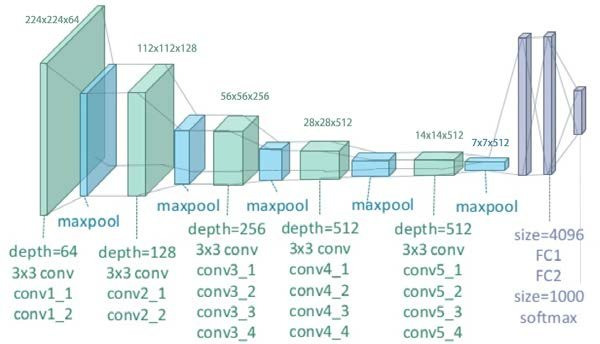
\includegraphics[width=0.80\textwidth]{vgg_19_img}
	\vspace*{-3mm}
	\caption[Aufbau des VGG19]{Der Aufbau des VGG19 \cite{VGG_19_IMG}.}
	\label{fig:vgg_19}
\end{figure}
\vspace*{-5mm}
Es ist zu beachten, dass sich Filter der selben Größe mehrfach wiederholen, sodass mit den vollständig verbundenen Schichten ein Konvolutionelles Neuronales Netz mit 19 Layern entsteht. Die vollständig verbundenen Schichten können in Keras ausgeschaltet werden, was in diesem Fall des Transfer Learning aufgrund der unterschiedlichen Zahl von nützlichen Ausgabeneuronen (das Netz sieht 1000 vor) sinnvoll ist. In der Entwicklung konnte das VGG19 mit angepassten vollständig verbundenen Schichten nahezu perfekt abschneiden. Dabei wurden in der Regel die originalen Schichten des VGG19 aus dem Lernvorgang ausgeschlossen, sodass die angelernten Features von diesem verwendet wurden, um die Zeichen der Hände in den folgenden vollständig verbundenen Schichten zu klassifizieren. Genauigkeiten von nahezu 100\% in der Validierung und in den Tests konnten durch das Transfer Learning erreicht werden. Dieses ist damit das am besten abschneidende Verfahren. Eines der genutzten Netze ist in folgender Abbildung zu erkennen:
\begin{figure}[H]
	\centering
	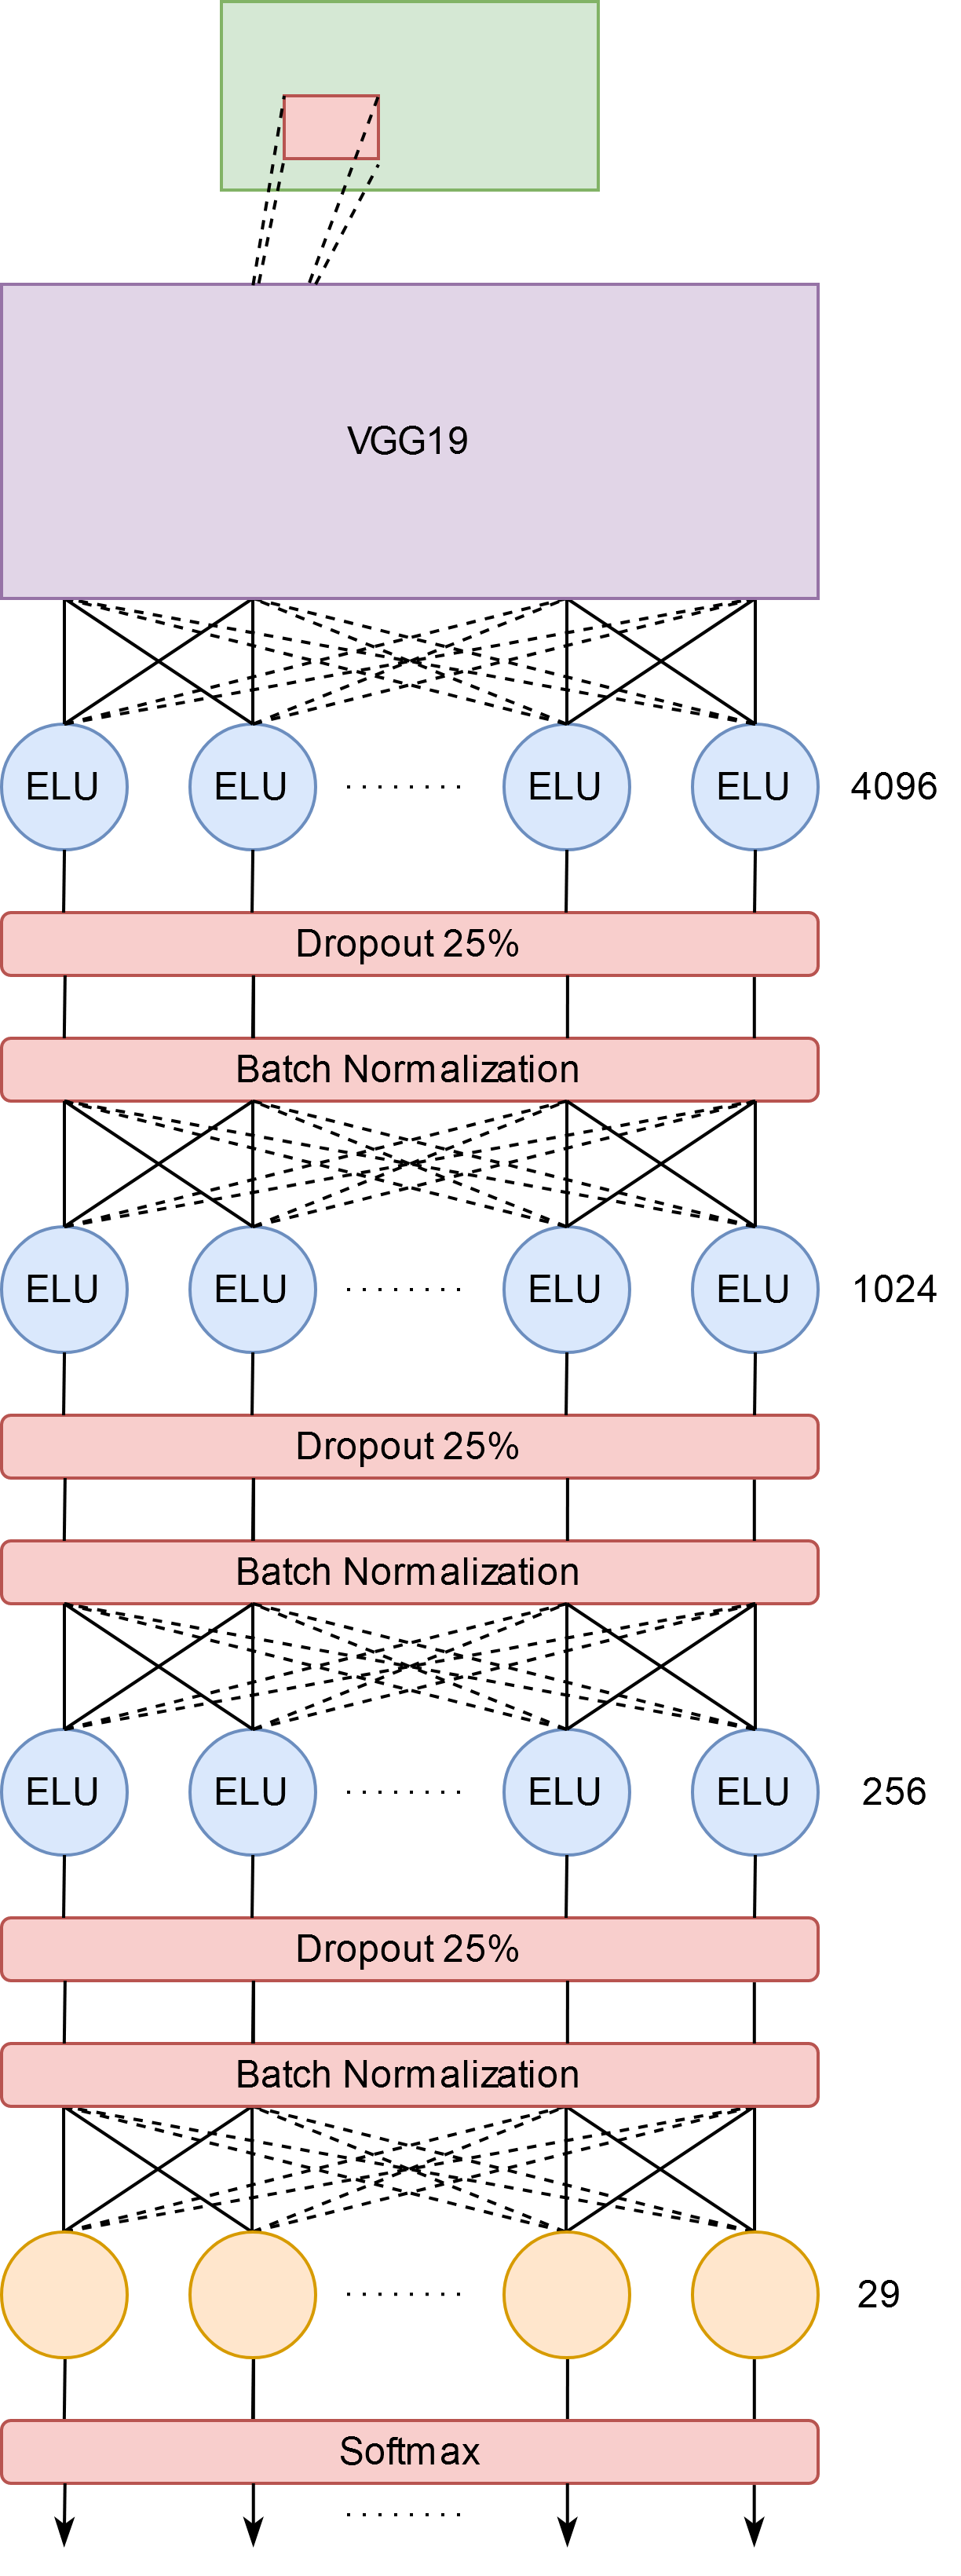
\includegraphics[width=0.60\textwidth]{vgg_19_used}
	\vspace*{-3mm}
	\caption[Angepasstes VGG19]{Angepasstes VGG19 mit sehr guten Ergebnisse.}
	\label{fig:vgg_19_used}
\end{figure}
\vspace*{-5mm}
\subsection{Backend der Webanwendung}
Das Backend es Projekts wurde mit Python implementiert um die ebenfalls mit Python trainierten Modelle einfach einbinden zu können. Die Programmiersprache Python wurde um die Bibliothek Flask ergänzt, welche erlaubt es mit wenig Aufwand HTTP Endpunkte zur Verfügung zu stellen. Das Backend dient dazu die trainierten Modelle für die Erkennung des Fingeralphabets über das Netzwerkprotokoll HTTP und die angesprochenen Endpunkte durch beliebige Clients nutzbar zu machen. Das in diesem Projekt implementierte Frontend nutzt die HTTP-Schnittstelle des Backends und kann also durch beliebige andere Clients aus dritter Hand ersetzt werden. Um Sicherzustellen, dass der Zugriff von externen Domains möglich ist, wird über Cross-Origin Ressource Sharing die Same-Origin Policy aufgeweicht. Die Same-Origin Policy wird von Browsern implementiert und schränkt den Zugriff auf eine Domain ein, sodass dieser nur von der gleichen Domain mit dem gleichen Port erfolgen kann.
\\\\
Einsprungspunkt des Python Backends ist die Datei \lstinline[language=pythoninline]|__init__.py|, welche Flask initialisiert und die durch Keras gespeicherten Modelle in eine globale Variable lädt. Genutzt wird dazu die Funktion \lstinline[language=pythoninline]|load_model| aus dem Import \lstinline[language=pythoninline]|tensorflow.keras.models| und das bewährte Dateiformat HDF5 (Hierarchical Data Format), welches auf die Speicherung großer Datenmengen in wissenschaftlichen Anwendungen zugeschnitten ist. Die geladenen Modelle werden in der Datei \lstinline[language=pythoninline]|services.py| als unterschiedliche HTTP-Endpunkte mit auf das Modell angepasste Parameter registriert. So muss beispielsweise je nach Input-Layer der Modelle das Bild eine gewisse Form aufweisen und die „Target-Shape“ wird so mit dem Modell hart verzahnt. 
\begin{lstlisting}[language=python,firstnumber=6,caption={Anlegen der HTTP-Endpunkte.},label=lst:add_http_endpoints]
# Gültige Urls für Modelle
model_urls = {
"150x150_5_Layer_CNN.hdf5": "/cnn_5_150_150",
"224x224_VGG19_CNN.hdf5": "/vgg19_224_224",
"224x224_VGG19_CNN_v2.hdf5": "/vgg19_224_224_v2"
}

# Infos der Modelle mit URLs zurückgeben
api.add_resource(ModelInfo, "/model_info", endpoint="model_info", resource_class_kwargs={"model_urls": model_urls})

# Eigenes Modell mit Eingangsgröße 150x150 und 5 CNN Layern.
api.add_resource(SignLanguageCNN, model_urls["150x150_5_Layer_CNN.hdf5"], endpoint="cnn_5_150_150",
resource_class_kwargs={"document_outputs": False,
"target_shape": (150, 150),
"model_config": app.config["MODELS"]["150x150_5_Layer_CNN.hdf5"]})

# VGG19 mit Eingangsgröße 224x224 umtrainiert.
api.add_resource(SignLanguageCNN, model_urls["224x224_VGG19_CNN.hdf5"], endpoint="vgg19_224_224",
resource_class_kwargs={"document_outputs": False,
"to_grayscale": False,
"target_shape": (224, 224),
"model_config": app.config["MODELS"]["224x224_VGG19_CNN.hdf5"]})

# VGG19 mit Eingangsgröße 224x224 umtrainiert und mit VGG19_Preprozess der Bilder.
api.add_resource(SignLanguageCNN, model_urls["224x224_VGG19_CNN_v2.hdf5"], "/default", endpoint="vgg19_224_224_v2",
resource_class_kwargs={"document_outputs": False,
"to_grayscale": False,
"target_shape": (224, 224),
"model_config": app.config["MODELS"]["224x224_VGG19_CNN_v2.hdf5"]})
\end{lstlisting}
Der oberste Endpunkt \lstinline[language=pythoninline]|/model_info| ist in der Datei \lstinline[language=pythoninline]|ModelInfo.py| ausprogrammiert und erlaubt es per HTTP-GET die hinterlegten Modelle und die dazugehörige URL abzufragen. So kann ein Client zwischen den Modellen hin und her wechseln. Gerade für das Testen im Real-Betrieb war das wichtig und die Unterschiedlichen Leistungen konnten leichter herausgearbeitet werden. Das Backend wurde unter \url{https://jupiter.fh-swf.de/sign-language} gehosted, sodass für die Abfrage der Modelle \url{https://jupiter.fh-swf.de/sign-language/model_info} per HTTP-GET angesprochen werden muss.
\begin{lstlisting}[language=python,firstnumber=4,caption={Abfrage der möglichen Modelle.},label=lst:request_models]
class ModelInfo(Resource):
"""
Resource, die URL Infos zu den Modellen zurückgibt.
"""
def __init__(self, model_urls):
"""
Resource, die URL Infos zu den Modellen zurückgibt.
:param model_urls: URL Infos, die zurückgegeben werden.
"""
self.model_urls = model_urls

def get(self):
"""
Gibt die Model Infos mittels get-Request zurück.
"""
return self.model_urls, 200
\end{lstlisting}
Der Hauptendpunkt ist in der Klasse \lstinline[language=pythoninline]|SignLanguageCNN| in der Datei \lstinline[language=pythoninline]|SignLanguageCNN.py|implementiert. Dieser erlaubt es per HTTP-POST ein Bild an das Backend zu senden, welches je nach URL (Siehe zwei Bilder drüber) durch ein unterschiedliches Netz geschoben wird. Als Parameter dienen \lstinline[language=pythoninline]|image| und \lstinline[language=pythoninline]|image_base_64|. Der Parameter \lstinline[language=pythoninline]|image_base_64| wurde eigens für das Frontend hinzugefügt, da die Bildextraktion aus einem HTML5 Canvas lediglich Base 64 kodiert gelingt. Je nach Modell ist eine Auswertung der Farbe nicht möglich, sodass das Bild nach der Anpassung der Größe auf den Input Layer noch in Graustufen umgewandelt wird.
\begin{lstlisting}[language=python,firstnumber=44,caption={Verarbeitung der Bilder im HTTP-Endpunkt.},label=lst:signlanguage_prediction]
# Image per FileStorage im Request
if args.image:
image = args.image
# Image per Base64 in Post
else:
image = BytesIO(base64.b64decode(args.image_base_64))

# Öffne das Bild und resize es.
image_pil = Image.open(image).resize(self.target_shape)
color_dim = 3

# Wenn Grauwert ausgewertet
if self.to_grayscale:
image_pil = image_pil.convert("L")
color_dim = 1
# Wenn RGB ausgewertet
else:
image_pil = image_pil.convert("RGB")

# Image in ein Tensorflow Array, Reshape es in 4 Dimensionen (BatchSize (1), Breite, Höhe, Farben)
image_tf = img_to_array(image_pil).reshape((1, self.target_shape[0], self.target_shape[1], color_dim))
# Prediction für das Bild, mit der genutzten Config.
prediction = self.model_config["MODEL"].predict(image_tf).tolist()

\end{lstlisting}
Das Ergebnis der Prediction ist eine Klassifizierung mit den jeweiligen Wahrscheinlichkeiten der zutreffenden Klasse. Der Wertebereich bewegt sich zwischen 0 und 1, wobei 1 als voll zutreffend gilt.  Das Ergebnis wird in ein Dictionary bestehend aus Klasse und Prediction-Value überführt und mit einem Statuscode 200 an den aufrufenden Client zurückgeschickt.
\subsection{Frontend der Webanwendung}
Das webbasierte Frontend dient als „Real-Welt-Anwendung“ um die Modelle außerhalb der Testdaten zu nutzen. Das Frontend wurde mithilfe von Angular, Angular Material und RxJS als Progressive Web APP programmiert und unter \url{https://jupiter.fh-swf.de/sign-language-classification/} zur Verfügung gestellt. Gehosted wird die Applikation sowie auch das Backend hinter einem nginx Webserver. Aufgeteilt wurde die Anwendung in die eigentliche Zeichenerkennung und einer Übersicht aller möglichen Handzeichen, erreichbar über das Menü in der Topbar. Die möglichen Handzeichen wurden mit Bildern modelliert, die die Hand von Vorne zeigen. Diese Bilder entstammen einem Icon-Set für das unter \ref{fingeralphabet} angesprochene amerikanische Fingeralphabet. Die tatsächliche Handstellung kann durch Rotation etwas abweichen, sodass Originalbilder einer menschlichen Hand in der Übersicht eingefügt wurden. Die Originalbilder stammen aus dem Trainingsdatensatz und sind über ein drüber fahren der Maus über das Handzeichen erreichbar. Die Auflösung der Originale ist mit 200x200 Pixeln nicht besonders hoch, aber ein erkennen der richtigen Handstellung ist Problemlos möglich. Die folgende Darstellung zeigt das d als Handzeichen als Icon und im Original.
\begin{figure}[H]
	\centering
	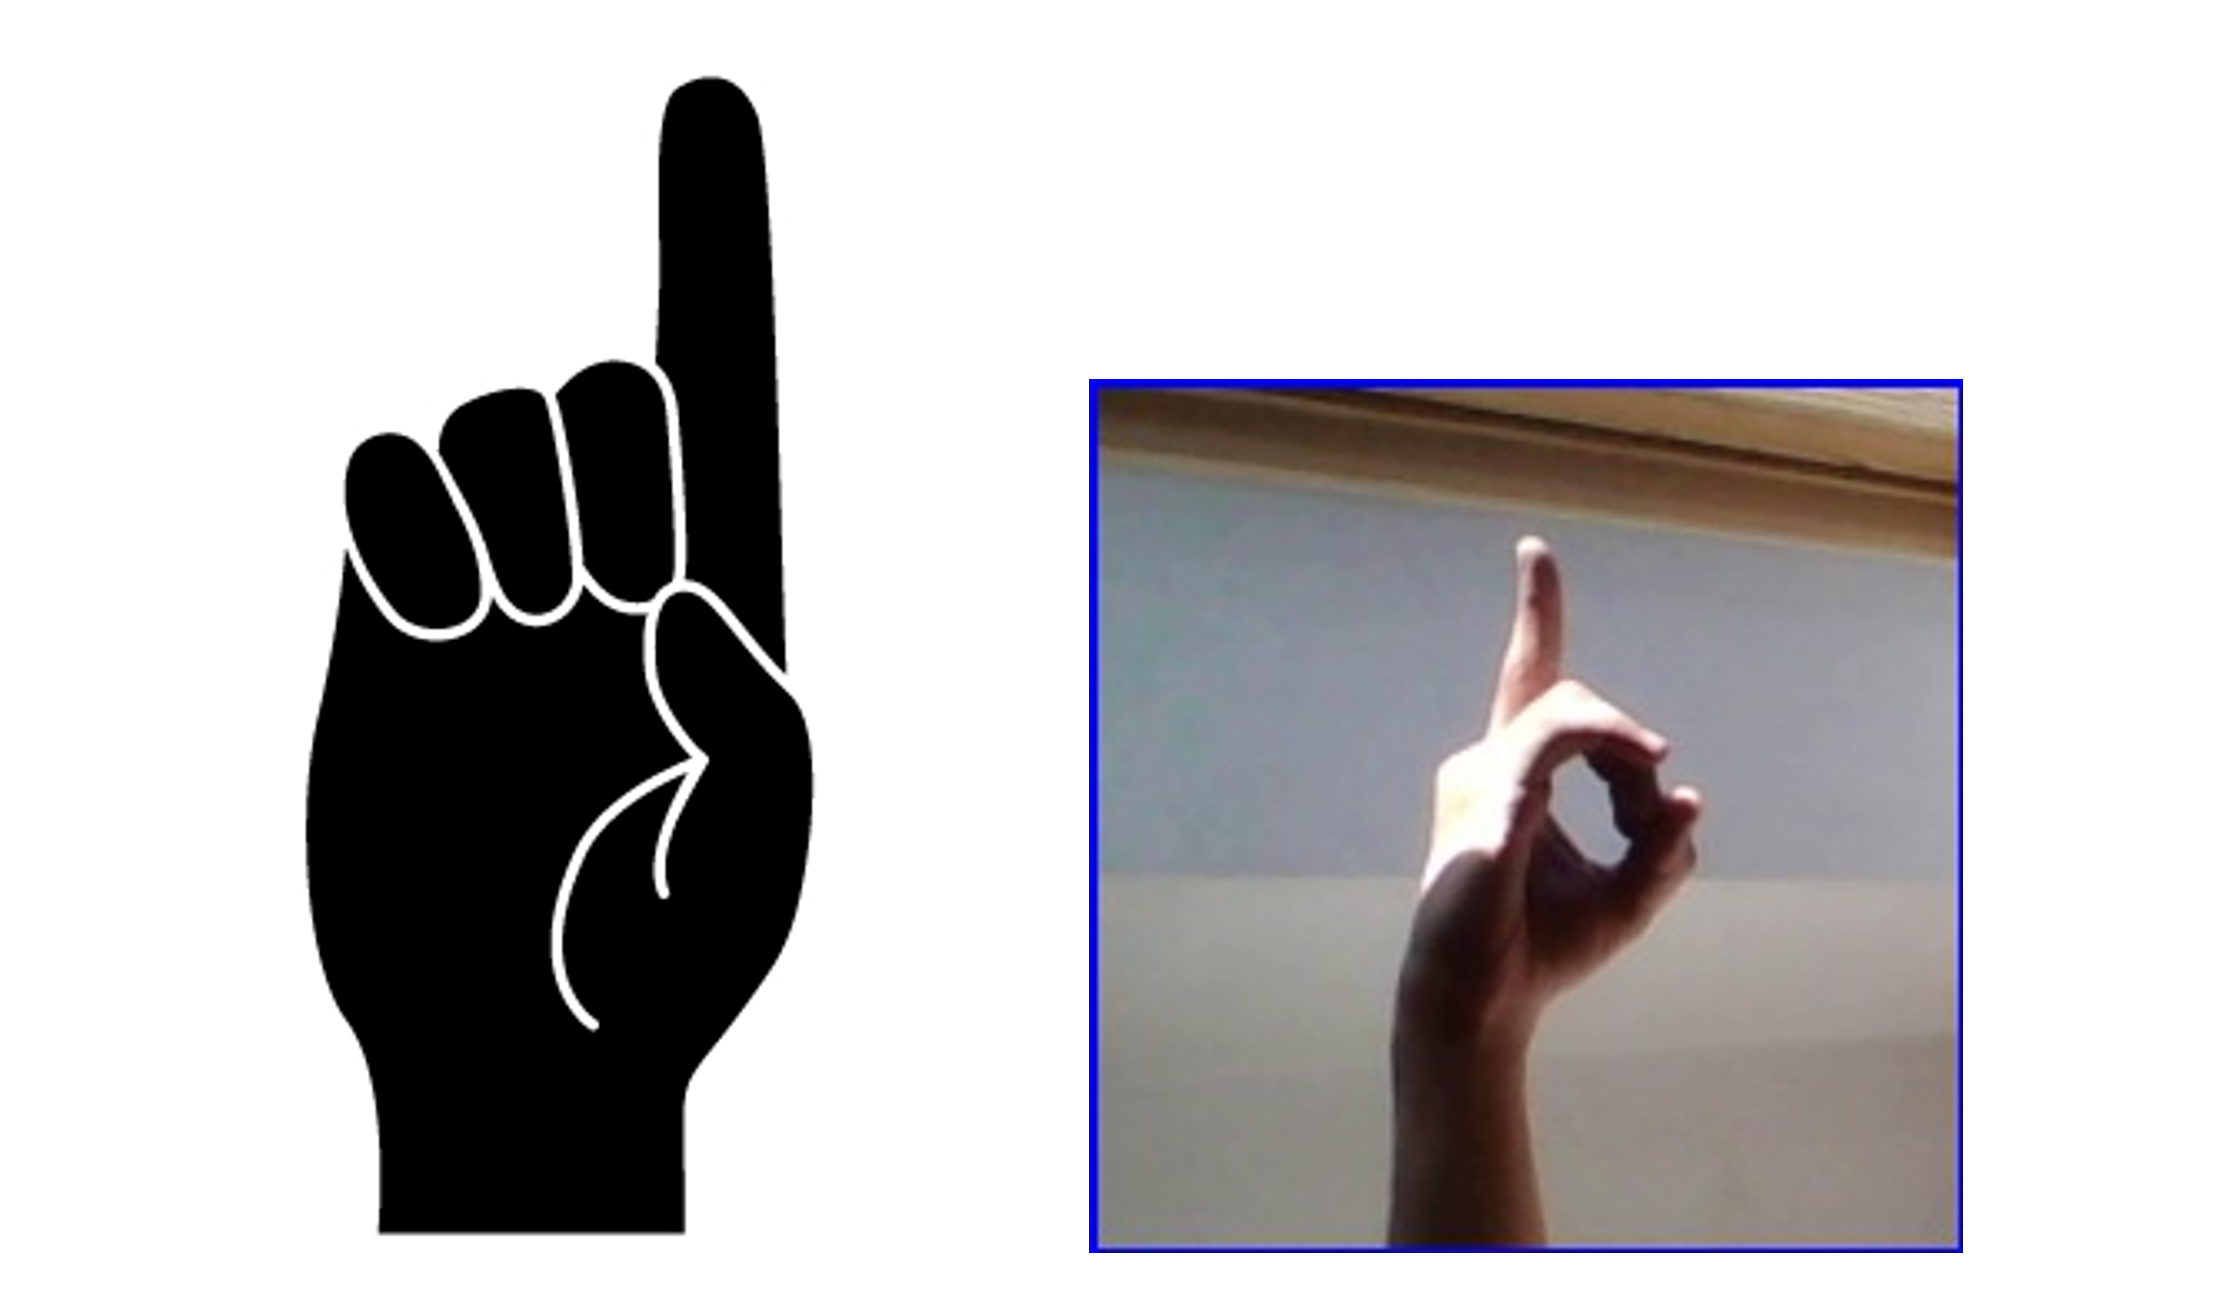
\includegraphics[width=0.80\textwidth]{d}
	\vspace*{-3mm}
	\caption[D als Handzeichen als Icon und im Original]{Das d als Handzeichen als Icon und im Original.}
	\label{fig:d}
\end{figure}
Auf der Seite für die Zeichenerkennung im Frontend kann mit dem Leerzeichen oder einem Klick auf „Start Prediction“ die Erkennung über eine Webcam gestartet werden. Der Zugriff auf die Webcam muss dabei aktiv vom Benutzer erlaubt werden. Frontendseitig wird mithilfe von Googles MediaPipe Hands die Hand im Bild in Echtzeit getracked. MediaPipe Hands besteht aus mehreren Modellen die über eine ML-Pipeline zusammenabreiten. Das erste Modell operiert auf dem gesamten Bild und findet die Handfläche. Das zweite Modell nutzt den Ausschnitt der gefundenen Handfläche und markiert 21 markante Punkte der Hand. MediaPipe Hands konnte mithilfe von TensorFlow.js Frontendseitig eingebunden und angesprochen werden. Das laden des Handtracking-Modells wird in der Datei \lstinline[language=pythoninline]|main.ts| durchgeführt und automatisch an das globale Window-Objekt gehangen.
\begin{lstlisting}[language=javascript,firstnumber=16,caption={Laden der frontendseitigen MediaPipe Hands Modelle.},label=lst:loading_mediapipe_hands_models]
(async () => {
const model = await handpose.load();
(window as any).tensorflowModel = model;
platformBrowserDynamic().bootstrapModule(AppModule)
.catch(err => console.error(err));
})();
\end{lstlisting}
Sobald das Modell Frontendseitig registriert wurde, wird die Angular Applikation gestartet. Da das Frontend sich die Bibliothek lediglich zu Nutze macht und in das trainieren in ein Handtracking-Modell keine Eigenleistung investiert wurde, wird technisch nicht tiefer auf MediaPipe Hands eingegangen. Das Bild der Webcam wird normalerweise in einem HTML5 Video-Element dem Benutzer angezeigt. Aber da auf so ein Element weder gezeichnet noch Einzelbilder extrahiert werden können, wurde für die Ausgabe ein Canvas-Element genutzt. Die Hauptaufgabe der Frontendseitigen Handerkennung passiert in der Datei \lstinline[language=pythoninline]|webcam.component.ts| unter \lstinline[language=pythoninline]|src/app/sign-prediction/webcam/| in der Methode \lstinline[language=pythoninline]|estimateHands|. Hier wird nach auslesen der Höhe und Breite des Video- und Canvas-Elements das Bild der Webcam in das Canvas übertragen. Dazu wird der Rendering-Context des Canvas-Elements genutzt und das Video-Element zuvor ausgeblendet. Über die zuvor angesprochene globale Variable kann auf das Handtracking-Modell zugegriffen werden und das aktuelle Webcam-Bild übergeben werden. Sollte eine Hand gefunden werden, werden die Koordinaten extrahiert und in einen mit RxJS erstellten Stream übergeben.
\begin{lstlisting}[language=javascript,firstnumber=124,caption={Erkennen einer Hand mit MediaPipe Hands.},label=lst:estimate_hands]
private async estimateHands() {

const videoWidth = this.video.nativeElement.videoWidth;
const videoHeight = this.video.nativeElement.videoHeight;
const canvasWidth = this.overlay.nativeElement.width;
const canvasHeight = this.overlay.nativeElement.height;

this.renderingContext.drawImage(
this.video.nativeElement, 0, 0, videoWidth, videoHeight, 0, 0, canvasWidth,
canvasHeight);

if (this.isPredictionActive) {
const model: HandPose = (window as any).tensorflowModel;
const hands: Array<any> = await model.estimateHands(this.video.nativeElement);
const boundingBox = hands.length > 0 ?
{ topLeft: hands[0].boundingBox.topLeft, bottomRight: hands[0].boundingBox.bottomRight } :
{ topLeft: ['0', '0'], bottomRight: ['0', '0'] };


this.croppedRenderingContext.clearRect(0, 0,
this.croppedCanvas?.nativeElement.width,
this.croppedCanvas?.nativeElement.height);

this.ngZone.run(() =>
this.boundingBoxSubject.next(boundingBox)
);
}

if (this.isPredictionActive) {
requestAnimationFrame(this.estimateHands.bind(this));
}
}
\end{lstlisting}
Mithilfe der \lstinline[language=pythoninline]|requestAnimationFrame| Methode, wird pro Frame die Methode \lstinline[language=pythoninline]|estimateHands| erneut aufgerufen, bis der Benutzer abbricht. Das Handtracking wird mithilfe von WebGL auf der Grafikkarte ausgeführt, sodass es ohne Grafikkarte zu FPS Einbrüchen kommen kann. Der RxJS Stream kümmert sich nachgelagert um das einzeichnen einer roten Box um die Hand des Benutzers.
\begin{figure}[H]
	\centering
	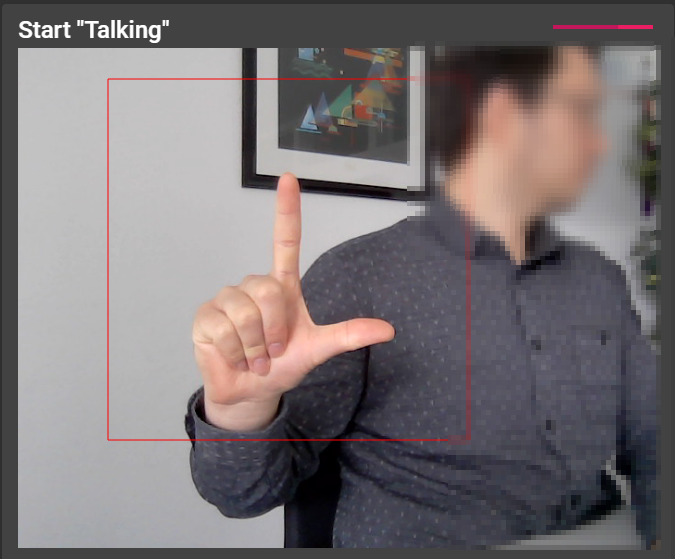
\includegraphics[width=0.80\textwidth]{webcam_image}
	\vspace*{-3mm}
	\caption[Bild der Webcam]{Bild der Webcam, welche an das Backend übertragen wird.}
	\label{fig:webcam}
\end{figure}
In einem 1.5 Sekunden-Intervall wird das aktuelle Bild der Webcam an das Python Backend übertragen und das Ergebnis im Frontend visualisiert. Da das trainierte Modell für das Fingeralphabet auch eine Klasse für „kein Handzeichen des Fingeralphabets“ hat, wird das Bild auch ohne erkannte Hand im Frontend übertragen. Sollte mit ablaufen des Intervalls im Frontend eine Hand erkannt worden sein, wird diese quadratisch anhand der Box ausgeschnitten. Dies erleichtert dem Anwender die Positionierung der Hand in eine möglichst optimale Hintergrundumgebung ohne ablenkende Objekte oder Farben. Diese Optimierung war nötig, da die Trainingsdaten stark auf die Hand fokussiert sind und Hintergründe mit markanten Formen die Erkennung trotz der automatischen Merkmalerkennung eines Konvolutionellen neuronalen Netzes beeinflusst haben. Das Intervall ist momentan nicht konfigurierbar und wurde als guter Mittelwert für ungeübte Nutzer des Fingeralphabets eingesetzt. Während des Betriebs kann das aktuelle Modell mit der Auswahlbox über der Webcam-Ausgabe gewechselt werden, ohne das Tracking zu beenden. 
\\\\
Neben den Koordinaten der Hand erkennt das frontendseitige Modell wie bereits erwähnt zusätzlich 21 Punkte auf der Hand, wodurch die Fingerstellung genau abgelesen werden kann.
\begin{figure}[H]
	\centering
	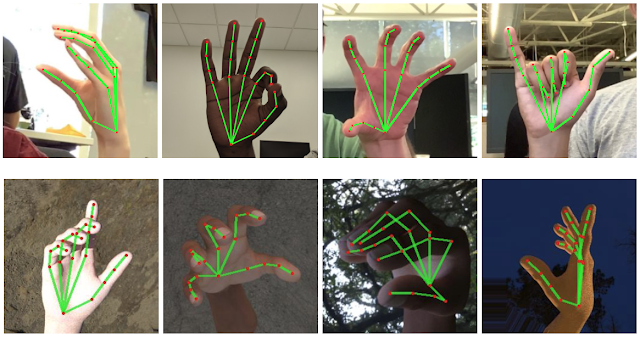
\includegraphics[width=0.80\textwidth]{mediapipe_finger}
	\vspace*{-3mm}
	\caption[Punktedarstellung eines Handzeichen in Mediapipe]{Punktedarstellung eines Handzeichen in Mediapipe.}
	\label{fig:mediapipe_finger}
\end{figure}
Dies hätte die Vorhersage des Fingeralphabets stark vereinfacht und die Bildverarbeitung ersetzen können. Da das Projekt aber mit Konvolutionellen neuronalen Netze auf Bildklassifizierung abzielt, wurde in diesem Projekt die Möglichkeit nicht berücksichtigt.
\subsection{Ergebnisse der Entwicklung}
Aufgrund der geringen Informationsdichte und der daraus vermutlich resultierenden schlechten „Real-Ergebnisse“ wurde der Sign Language MNIST Datensatz schnell verworfen. Für den ASL Alphabet Datensatz wurde per zufälligem Ziehen ein Testdatensatz mit 300 Elementen angelegt. Auf Basis der Ordner-Struktur konnte mit der Funktion \lstinline[language=pythoninline]|image_dataset_from_directory| zügig ein Dataset zum Trainieren eines Modells erstellt werden. Sämtliche Trainingsläufe wurden wie unter 5.1.2 beschrieben geloggt und konnten so jederzeit nachvollzogen und erneut erzeugt werden. Die einfachen neuronalen Netze konnten lediglich auf dem kleinen Sign Language MNIST Datensatz sinnvoll trainiert werden. Die Vorhersagengenauigkeit lag je nach Datensatz aber lediglich zwischen 67\% und 81\% auf den jeweiligen Testdaten. Die trainierten Konvolutionellen Neuronalen Netze konnten auf dem ASL Alphabet Datensatz über 99\% Vorhersagengenauigkeit auf Test- und Validierungsdaten erreichen und wurden nur mithilfe von Transfer Learning eines VGG19 Modells überboten. Die guten Ergebnisse waren wenig überraschend, da CNNs als defacto Standard für Bildverarbeitung gelten. Auch eine Konfusionsmatrix zeigt, dass es unter den sehr geringen Fehlern keine besonderen Ausreißer gibt, obwohl sich einige Buchstaben recht ähnlich sind.  Somit wurde das VGG19 Modell als Standard im Frontend hinterlegt. Das Python Backend ist in der Lage die unterschiedlichen Modelle in den Speicher zu laden und Bilder mit und ohne Base 64 Kodierung zu verarbeiten. Die Modelle sind über unterschiedliche Endpunkte per HTTP direkt ansprechbar und eine Prediction dauert unter 100ms Millisekunden. Die im Backend hinterlegten Modelle können abgefragt werden.  Das Frontend visualisiert die möglichen Handzeichen und ist in der Lage über die Webcam und MediaPipe Hands die Hand zu tracken. In einem Intervall von 1.5 Sekunden wird das aktuelle Bild an das Backend übertragen und das Ergebnis dem Benutzer angezeigt. Damit konnte die geplante Entwicklung im Rahmen dieses Projekts erfolgreich abgeschlossen werden.
\section{Fazit} 
Das Projekt hat neben den theoretischen Grundlagen von Machine Learning, einfache Neuronale Netze, Konvolutionelle Neuronale Netze und Transfer Learning näher beleuchtet. Die besten Modelle erreichten nahezu 100\% Vorhersagegenauigkeit auf Test- und Validierungsdaten. Darüber hinaus wurden die Modelle in eine Anwendung integriert und die Vorhersagen auf echten Daten zu prüfen. Trotz der ausgezeichneten Ergebnisse auf den Datensätzen zeigen sich schwächen mit Echt-Daten. Eine richtige Vorhersage der Handzeichen kann mit etwas Übung des Benutzers zwar erreicht werden, aber die Positionierung vor der Webcam nimmt noch zu großen Einfluss. Markante Formen und Farben die in den Bildausschnitt der Hand hineinragen erschweren zusätzlich die Erkennung, sodass der Benutzer nach Möglichkeit einen ruhigen Hintergrund wählen sollte. Auch wenn die aus diesem Projekt hervorgegangene Applikation noch nicht für eine reale Nutzung vollends geeignet ist, sind die End-Ergebnisse zufriedenstellend. Vor allem mit dem Hintergrund, dass die Applikation bestehend aus Frontend und Backend vordergründig als On-Top Ergänzung zu den trainierten Modellen gedacht war. Uns war es aber wichtig in diesem Projekt eine Applikation zu implementieren, da die Schwierigkeit beim Machine Learning gerade darin besteht, die Modelle Praxis-Tauglich aus dem Test-Labor in die echte Welt zu übertragen.   
\section{Ausblick}
Während der Planung und Entwicklung des Projekts sind einige Punkte aufgefallen, die zur Verbesserung zusätzlich umgesetzt werden könnten. Um im Rahmen des Projektumfangs zu bleiben, werden diese anschließend nur in schriftlicher Form vorgestellt.
\subsection{Data Augmentation}
Der genutzte ASL Alphabet Datensatz hat mit 87000 Bildern bereits eine angemessene Größe. Die Bilder scheinen allerdings alle von einer Person erzeugt worden zu sein. Die Bilder für einen Buchstaben unterscheiden sich zwar stärker als im Sign Language MNIST Datensatz, aber dennoch deutlich weniger als mit unterschiedlichen Personen. So könnten die Bilder manuell rotiert und umpositioniert werden, um einen breiteren Datensatz zu erzeugen und so ein besseres Ergebnis auf „Real-Daten“ zu erhalten.
\subsection{Ausbau des Traingsdatensatzes}
Alternativ zur Data Augmentation könnte der Datensatz durch Real-Daten erweitert werden. Das Frontend sendet sämtliche Bilder Base 64 kodiert an das Python Backend. Diese Bilder könnten gespeichert und manuell klassifiziert werden. Auf lange Sicht könnte der bestehende Datensatz sogar ersetzt werden um das Ergebnis an den Bildern der Webcam anzupassen und zu verbessern.
\subsection{Perfomance des Frontends}
Das Frontend arbeitet selbst mit einem großen Modell mithilfe von TensorFlow.js, um die Hand in dem Bild der Webcam zu finden. Dies erlaubt es dem Benutzer Feedback zu geben und die Hand bereits Frontendseitig auszuschneiden. Das Modell wird mit WebGL direkt auf der Grafikkarte ausgeführt und wird mit dem Start der Applikation geladen. Insgesamt werden ca. 15MB übertragen, welche für eine durchschnittliche Interleitung keine Probleme darstellen. Dennoch könnte die Startzeit der Applikation mit geringerer Dateigröße verringert werden. Außerdem ist eine dedizierte Einsteiger-Grafikkarte vorauszusetzen um ein flüssiges Arbeiten zu garantieren. Mit dem Verzicht auf das Handtracking, könnte das Modell wegfallen und die Aufbereitung aus dem Frontend in das Backend übertragen werden. So wäre ein flüssiges Arbeiten mit dem Frontend auf nahezu jeder Hardware möglich.
\subsection{Textausgabe im Frontend}
Momentan wird im Frontend der erkannte Buchstabe hervorgehoben. Das trainierte Modell bietet zusätzlich noch die Klassen Space und Delete, die dazu genutzt werden könnten eine sinnvolle Textausgabe auf Basis der Vorhersagen zu realisieren. 
\subsection{Intervall der Handzeichenerkennung}
Zurzeit ist das Intervall in dem das Bild der Webcam an das Backend übertragen wird auf ungeübte Nutzer ausgelegt. Dank der geringen Antwortzeit des Backends von unter 100ms, könnte das Intervall deutlich verringert werden. Dadurch wäre ein deutlich flüssigeres Arbeiten mit dem Frontend möglich. Alternativ könnte auf das Intervall gänzlich verzichtet werden, indem das frontendseitige Handtracking als Grundlage genutzt wird. Dazu könnte ein gewisses Delta für die Handkoordinaten im Bild festgelegt werden. Sobald dieses Delta überschritten wurde, wird ein neues Zeichen oder ein wiederholtes gleiches Zeichen angenommen und das Backend angesprochen. 
\setcounter{biburllcpenalty}{7000}
\setcounter{biburlucpenalty}{8000}
\pagebreak
\printbibliography[title=Quellen]
\end{document}